\documentclass{book}[11pt]
\usepackage[a4paper, total={4.75in, 7in}]{geometry}
\usepackage{graphicx,epstopdf}	
\usepackage{parallel}
\usepackage{amsmath}
\usepackage{pdflscape}

\usepackage{fontspec}
%\setmainfont{Times New Roman}[Scale=MatchLowercase]
\setmainfont{EB Garamond}[Scale=0.955]
\usepackage{polyglossia}
\setmainlanguage{english}
\setotherlanguage{greek}
\newfontfamily\greekfont{Times New Roman}

\usepackage{titlesec}
\titleformat{\chapter}
  {\normalfont\huge\bfseries\centering}
  {\thechapter.}
  {0.5em}
  {}            
\titlespacing*{\chapter}{0pt}{-20pt}{40pt}

\titleformat{\section}
  {\normalfont\Large\itshape\centering}
  {\thesection}
  {1em}
  {}

\usepackage{fancyhdr}
\pagestyle{fancy}
\fancyhf{} 
\fancyhead[LE,RO]{\thepage}
\fancyhead[CE]{FITZPATRICK}
\fancyhead[CO]{{\em Modern Almagest},\, \MakeUppercase{\leftmark}}

\newcommand {\btau}{\mbox{\boldmath$\tau$}}
\newcommand {\bOmega}{\mbox{\boldmath$\Omega$}}
\newcommand {\bomega}{\mbox{\boldmath$\omega$}}

\renewcommand{\chaptermark}[1]{\markboth{\thechapter. #1}{}}
\addto\captionsenglish{%
  \renewcommand{\contentsname}{Table of Contents}
}
%\renewcommand{\chaptermark}[1]{\markboth{#1}{}}

\setlength{\tabcolsep}{3.5pt} 

\begin{document}
%\fontsize{10pt}{11pt}\selectfont

\title{A MODERN ALMAGEST:\\[0.5ex]An Updated  Version of Ptolemy's Model of the Solar System}
\author{Richard Fitzpatrick}
\date{}
\maketitle

\frontmatter
\tableofcontents
\chapter*{Preface}
\addcontentsline{toc}{chapter}{Preface}
% !TEX root = ./Almagest.tex
This book is devoted to a re-examination of Claudius Ptolemy’s Almagest, one of the foundational scientific works of antiquity. Although often contrasted 
unfavorably with Euclid’s Elements, and frequently dismissed as overly complex and misguided in its geocentric approach, the Almagest remains a remarkable 
achievement:  namely, a mathematically sophisticated and observationally grounded attempt to describe the motions of the heavens.
The aim of the present work is to reassess the scientific merits of Ptolemy’s model by reconstructing it in a modern framework. Using contemporary mathematical 
methods, as well as standard astronomical conventions and terminology, we seek to render the structure and logic of the Ptolemaic system more accessible to the 
modern reader. In doing so, we show that many common criticisms of the Almagest are either overstated or based on misunderstandings, and that, when properly 
interpreted, Ptolemy’s model can be viewed as a reasonably accurate  approximation to the later Keplerian description of planetary motion.
At the same time, this book does not attempt to reproduce every aspect of the original treatise. Rather than revisiting the construction of trigonometric tables or 
ancient observational techniques, we focus on the essential geometric and kinematic ideas underlying the model. Certain known deficiencies in Ptolemy’s system 
are corrected, and, where appropriate, his methods are reformulated in terms of equivalent but more transparent schemes.
The result is a streamlined yet faithful reconstruction of the Ptolemaic system—one that preserves its historical character while demonstrating its continued 
mathematical and scientific interest. It is hoped that this approach will allow readers to better appreciate both the ingenuity of Ptolemy’s achievement and its
 place in the development of astronomical science.\\
 ~\\
 \begin{flushright}
 Richard Fitzpatrick\\[0.5ex]
 {\em The University of Texas at Austin}
 \end{flushright}

\mainmatter
\include{Chapter01.tex}
\include{Chapter02.tex}
\chapter{Dates and times}
% !TEX root = ./Almagest.tex

\section{Julian and Gregorian calendars}
The Julian calendar was instituted by Julius Caesar in 45 BC. However, it was not correctly implemented until
8 AD. The Julian calendar assumes that the length of a tropical year (that is, the time between successive passages of the Sun through the vernal equinox) is $365.25$ days. 
Unfortunately, the true length of the tropical year is $365.2422$ days. This slight error caused the date of the vernal equinox to regress through the calendar over the course
of many centuries. In order to correct this problem, the Gregorian calendar was promulgated by Pope Gregory XIII in 1582. The new calendar was immediately adopted by all of the Catholic counties in Europe, and was eventually
(in some cases, after a delay of hundreds of years)
also adopted by all of the Protestant countries. According to the Gregorian calendar, the length of a tropical year is $365.2425$ days, which is very close to the correct length. 

\section{Julian day number}
Following modern astronomical practice, we shall specify dates  in this treatise 
by means of {\em Julian day numbers}. According to this
scheme, days are numbered consecutively from January 1, 4713 BC (in the Julian calendar), which
is designated day zero. For instance, October 14, 1066 AD (the Julian date of the battle of Hastings) is
day 2\,110\,701. Each Julian day commences at 12:00 universal time (UT). (Universal time is virtually identical to
Greenwich mean time.)

\section{Determination of Julian day numbers}
The Julian day number of a given day can be determined from Tables~\ref{kt1}--\ref{kt3}.  The
date must be expressed in terms of the Gregorian calendar. 

The procedure is as follows:
\begin{enumerate}
\item Enter the table of century years (Table~\ref{kt1}) with the century
year immediately preceding the  date in question, and take out the tabular
value. If the
century year is marked with a $\dag$, note this fact for use in step 2.
\item Enter the table of years of the century (Table~\ref{kt2}) with the
last two digits of the year in question, and take out the tabular value.
If the century year used in step 1 was marked with a $\dag$, diminish the tabular value
by one day, unless the tabular value is zero. If the year in question
is a leap year,  marked with a $\ast$, note this fact for use in step 3.

\item Enter the table of the days of the year (Table~\ref{kt3}) with the
day in question, and take out the tabular value. If the year in question
is a leap year and the table entry falls after February 28, add
one day to the tabular value. The sum of the values obtained
in steps 1, 2, and 3 then gives the Julian day number of the date in question.
\end{enumerate}

~\\
\noindent {\em Example~1}: June 10, 1992 AD:\\~\\
\begin{tabular}{lrrr}
1.~Century year & $^\dag1900$ &&$2\,415\,020$\\
2.~Year of the century & $^\ast92$ & $33\,603 - 1 =$& $33\,602$\\
3.~Day of the year & June 10 & $161+1 =$ & $162$\\\cline{4-4}
Julian day number&&&$2\,448\,784$\\
&&&\\
\end{tabular}\\
Observe that in step 2 the tabular value has been diminished by 1 because 1900
is a common year (marked with a $\dag$ in Table~\ref{kt1}). In step 3, the
tabular value has been increased by 1 because 1992 is a leap year (marked with a $\ast$ in Table~\ref{kt2}), and the
date falls after February 28.

~\\
\noindent {\em Example~2}: January 18, 1824 AD:\\~\\
\begin{tabular}{lrrr}
1.~Century year & $^\dag1800$ &&$2\,378\,496$\\
2.~Year of the century & $^\ast24$ & $8\,766 - 1=$ & 8\,765\\
3.~Day of the year & January 18 & $18 =$ & $18$\\\cline{4-4}
Julian day number&&&$2\,387\,279$\\
&&&\\
\end{tabular}\\
Observe that in step 2 the tabular value has been diminished by 1 because 1800
is a common year (marked with a $\dag$ in Table~\ref{kt1}). In step 3, the
tabular value has not been increased by 1, despite the fact that 1824 is a leap year (marked with an $\ast$ in Table~\ref{kt2}),  because the
date falls before February 28.

We can specify the time of day (in universal time), as well as the date, 
by means of fractional Julian day numbers. For instance,
$t=2\,448\,784.0$ JD corresponds to 12:00 UT  on  June 10, 1992 AD, whereas
$t=2\,448\,784.5$ JD corresponds to 24:00 UT later the same day.

\section{Tables}

\begin{table}[b]\centering
\begin{tabular}{rr}
$^\dag$1700 &  $2\,341\,972$\\
 $^\dag$1800 &  $2\,378\,496$\\
 $^\dag$1900 & $2\,415\,020$\\
 2000 & $2\,451\,544$\\
 $^\dag$2100 & $2\,488\,069$\\
 $^\dag$2200 & $2\,524\,593$\\
  $^\dag$2300 & $2\,561\,117$
\end{tabular}
\caption {Julian Day Number: Century Years. $^\dag$\,Common years. All years are AD. Table reproduced, with permission, from Evans (1998).}\label{kt1}
\end{table}

\vspace*{1cm}

\begin{table}[h]\centering
\begin{tabular}{rr|rr|rr|rr|rr}
$^\S$0 & $0$ & $^\ast$20 & $7\,305$ & $^\ast$40 & $14$\,610 & $^\ast$60 &$21\,915$ & $^\ast$80 & $29\,220$\\
1 & $336$ & 21 & $7\,671$ & 41 & $14\,976$ & 61 &$22\,281$ & 81& $\,29\,586$\\
2 & $731$ & 22 & $8\,036$ & 42 & $15\,341$ & 62 & $22\,646$ & 82 & $29\,951$\\
3 & $1\,096$ & 23 & $8\,401$ & 43 & $15\,706$ & 63 & $22\,011$& 83 &$ 30\,316$\\
&&&&&&&\\
$^\ast$4& $1\,461$& $^\ast$24& $8\,766$& $^\ast$44 & $16\,071$ & $^\ast$64 & $23\,376$& $^\ast$84 & $30\,681$\\
5 & $1\,827$ & 25 & $9\,132$& 45 & $16\,437$& 65& $23\,742$& 85& $31\,047$\\
6& $2\,192$& 26& $9\,497$& 46& $16\,802$& 66& $24\,107$& 86& $31\,412$\\
7& $2\,557$&27&$9\,862$ & 47 & $17\,167$& 67& $24\,472$& 87& $31\,777$\\
&&&&&&&\\
$^\ast$8 & $2\,922$& $^\ast$28 & $10\,227$ & $^\ast 48$ & $17\,532$ & $^\ast 68$ & $24\,837$& $^\ast$88& $32\,142$\\
9 & $3\,288$& 29 & $10\,593$& 49& $17\,898$& 69& $25\,203$& 89& $32\,508$\\
10& $3\,653$& 30 & $10\,958$& 50& $18\,263$& 70& $25\,568$& 90& $32\,873$\\
11& $4\,018$& 31& $11\,323$& 51& $18\,628$& 71& $25\,933$& 91& $33\,238$\\
&&&&&&&\\
$^\ast$12& $4\,383$& $^\ast$32 & $11\,688$ & $^\ast$52 & $18\,993$ &
$^\ast$72 & $26\,298$ & $^\ast$92 & $33\,603$\\
13 & $4\,749$ & 33 & $12\,054$& 53& $19\,359$ & 73& $26\,664$ & 93& $33\,969$\\
14 & $5\,114$ & 34 & $12\,419$ & 54 & $19\,724$ & 74& $27\,029$ & 94&$34\,334$\\
15& $5\,479$ & 35& $12\,784$& 55 & $20\,089$ & 75& $27\,394$ & 95 & $34\,699$\\
&&&&&&&\\
$^\ast$16 & $5\,844$& $^\ast$36& $13\,149$& $^\ast$56 & $20\,454$& $^\ast$76&$27\,759$ & $^\ast$96& $35\,064$\\
17& $6\,210$& 37& $13\,515$& 57& $20\,820$& 77& $28\,125$& 97& $35\,430$\\
18& $6\,575$& 38& $13\,880$& 58& $21\,185$& 78& $28\,490$& 98& $35\,795$\\
19& $6\,940$& 39& $14\,245$& 59& $21\,550$& 79& $28\,855$& 99&$36\,160$\\
\end{tabular}
\caption{Julian Day Number: Years of the Century. $^\ast$\,Leap year. $^\S$\,Leap year unless century is marked $^\dag$. In centuries marked $^\dag$, subtract one day from the tabulated values for the years 1 through 99.
Reproduced, with permission, from Evans (1998).}\label{kt2}
\end{table}

\newpage
\begin{table}[h]\centering
\begin{tabular}{r|rrrrrrrrrrrr}
Day & Jan & Feb & Mar & Apr & May & Jun & Jul & Aug & Sep & Oct& Nov & Dec\\\hline
&&&&&&&&&&&&\\[-1.5ex]
1 & 1 & 32 & 60 & 91 & 121& 152 & 182& 213& 244 & 274& 305& 335\\
2 & 2 & 33 & 61 & 92 & 122& 153& 183& 214& 245& 275& 306& 336\\
3 & 3&34 & 62& 93& 123& 154& 184& 215& 246& 276& 307& 337\\
4& 4& 35& 63& 94& 124& 155& 185& 216& 247& 277& 308& 338\\
5& 5&36& 64& 95& 125& 156& 186& 217& 248& 278& 309& 339\\
&&&&&&&&&&&&\\
6&6& 37& 65& 96& 126& 157& 187& 218& 249& 279& 310& 340\\
7&7 & 38 & 66 & 97& 127& 158& 188& 219& 250& 280& 311& 341\\
8& 8&39& 67& 98& 128& 159& 189& 220&251& 281& 312& 342\\
9&9&40&68&99&129& 160& 190& 221& 252& 282& 313& 343\\
10&10&41&69&100&130& 161& 191& 222& 253& 283&314&344\\
&&&&&&&&&&&&\\
11&11&42&70& 101& 131& 162& 192& 223& 254& 284& 315& 345\\
12& 12&43&71&102& 132& 163& 193& 224& 255& 285& 316& 346\\
13& 13& 44& 72& 103& 133&164& 194& 225& 256& 286& 317& 347\\
14& 14&45& 73& 104& 134& 165& 195& 226& 257& 285& 318& 348\\
15&15&46& 74& 105& 135& 166& 196& 227& 258& 288& 319& 349\\
&&&&&&&&&&&&\\
16& 16& 47& 75& 106& 136& 167& 197& 228& 259& 289& 320& 350\\
17& 17 & 48& 76& 107& 137& 168& 198& 229& 260& 290& 321& 351\\
18& 18& 49& 77& 108&138& 169& 199& 230& 261& 291& 322& 352\\
19& 19& 50& 78& 109& 139&170& 200& 231& 262& 292& 323& 353\\
20 & 20& 51& 79& 110& 140& 171& 201& 232& 263& 293& 324& 354\\
&&&&&&&&&&&&\\
21 & 21 & 52 & 80 & 111& 141& 172& 202& 233& 264& 294& 325& 355\\
22& 22& 53& 81& 112& 142& 173& 203& 234& 265& 295& 326& 356\\
23& 23& 54& 82& 113& 143& 174& 204& 235& 266&296& 327& 357\\
24& 24& 55& 83& 114& 144& 175& 205& 236& 267& 297& 328& 358\\
25&25&56& 84& 115& 145& 176& 206& 237& 268& 298& 329& 359\\
&&&&&&&&&&&&\\
26& 26& 57& 85& 116& 146& 177& 207& 238& 269& 299& 330& 360\\
27& 27& 58& 86& 117& 147& 178& 208& 239& 270& 300& 331& 361\\
28& 28& 59& 87& 118&148& 179& 209& 240& 271& 301& 332& 362\\
29&29&$\ast$&88&119& 149& 180& 210& 241& 272& 302& 333& 363\\
30&30&&89&120&150& 181& 211& 242& 273& 303& 334& 364\\
31&31&&90&&151&&212&243&&304&&365\\
\end{tabular}
\caption{Julian Day Number: Days of the Year. $\ast$\,In leap year,
after February 28, add 1 to the tabulated value. Reproduced, with permission, from Evans (1998).}\label{kt3}
\end{table}

\chapter{Geometric planetary orbit models}\label{ckep}
% !TEX root = ./Almagest.tex

\section{The model of Kepler}
In this chapter, 
 Kepler's geometric model of  a geocentric planetary orbit is  examined in detail, and then compared to the 
less accurate geometric models of Hipparchus, Ptolemy, and Copernicus. In the following,
all orbits are viewed from the  northern ecliptic pole.

Kepler's geometric model of a heliocentric planetary orbit is summed up in his   three well-known laws of planetary motion.
According to Kepler's first law, all planetary orbits are ellipses  that are  confocal with the Sun and lie in a
fixed plane.
Moreover, according to Kepler's second law, the radius vector which connects the Sun to a given planet sweeps out  equal areas in equal time intervals. 

\begin{figure}[h]
\centerline{\includegraphics[height=2.in]{Fig4-1.eps}}
\caption{A Keplerian orbit.}\label{jf1}
\end{figure}

Consider Figure~\ref{jf1}. The curve $\Pi PBA$ is half  of an elliptical planetary orbit. Furthermore, $C$ is the
geometric center of the orbit, $S$ the focus at which the Sun is located,
$P$ the instantaneous position of the planet, $\Pi$ the perihelion point (that is, the planet's point of closest approach to the Sun),
and $A$ the aphelion point (that is, the  point of furthest distance from the Sun). The ellipse is symmetric about
$\Pi A$, which is termed the {\em major axis}, and about $CB$,
which is termed the {\em minor axis}.
The length $CA\equiv a$ is called the orbital
{\em major radius}. The length $CS$  represents the displacement of the Sun from
the geometric center of the orbit, and is generally written $e\,a$, where $e$ is termed the
orbital {\em eccentricity}, and $0\leq e\leq 1$. The length $CB\equiv b = a\,(1-e^2)^{1/2}$ is called
the orbital {\em minor radius}. 
The length $SP\equiv r$ represents the radial distance of the planet from the Sun.
Finally, the angle $RSP\equiv T$ is the angular bearing of the planet from the Sun,
relative to the major axis of the orbit, and is termed the {\em true anomaly}. 

The curve $\Pi QDA$ is half of a circle whose geometric center is $C$, and whose
radius is $a$. Hence, the circle passes through the perihelion and aphelion
points. $R$ is the point at which the perpendicular from $P$ 
meets the major axis $\Pi A$. The point where $RP$ produced
meets circle $\Pi QDA$ is denoted $Q$. Finally,
the angle $SCQ\equiv E$ is called the {\em elliptic anomaly}. 

Now, the equation of the ellipse $\Pi PBA$ is
\begin{equation}
\frac{x^2}{a^2}+ \frac{y^2}{b^2} = 1,
\end{equation}
where $x$ and $y$ are the perpendicular distances from the minor and major
axes, respectively. Likewise, the equation of the circle $\Pi QDA$ is
\begin{equation}
\frac{x'^{\,2}}{a^2} + \frac{y'^{\,2}}{a^2} = 1.
\end{equation}
Hence, if $x=x'$ then
\begin{equation}
\frac{y}{y'} = \frac{b}{a},
\end{equation}
and it follows that
\begin{equation}\label{je4}
\frac{RP}{RQ} = \frac{b}{a}.
\end{equation}

Now, $CS = e\,a$. Furthermore, it is easily demonstrated that
 $SR=r\,\cos T$, $RP=r\,\sin T$, $CR= a\,\cos E$, and $RQ= a\,\sin E$. Consequently, Equation~(\ref{je4}) yields
\begin{equation}\label{je5}
r\,\sin T = b\,\sin E = a\,(1-e^2)^{1/2}\,\sin E.
\end{equation}
Also, because $SR = CR-CS$, we have
\begin{equation}\label{je6}
r\,\cos T = a\,(\cos E - e).
\end{equation}
Taking the square root of the sum of the squares of the previous two equations, we obtain
\begin{equation}\label{je7}
r = a\,(1-e\,\cos E),
\end{equation}
which can be combined with Equation~(\ref{je6}) to give
\begin{equation}
\cos T = \frac{\cos E - e}{1-e\,\cos E}.
\end{equation}

Now, according to Kepler's second law,
\begin{equation}
\frac{{\rm Area}\,\Pi PS}{\pi\,a\,b} = \frac{t-t_\ast}{\tau},
\end{equation}
where $t$ is the time at which the planet passes point $P$,  $t_\ast$  the time at which it passes the perihelion point,
and $\tau$ the {\em orbital period}.
However,
\begin{align}
{\rm Area}  \,\Pi PS &= {\rm Area}\, SRP + {\rm Area} \,\Pi RP
= \frac{1}{2}\,r^2\,\cos T\,\sin T + {\rm Area}\,\Pi RP.
\end{align}
But,
\begin{equation}
{\rm Area}\,\Pi RP = \frac{b}{a}\,{\rm Area}\,\Pi RQ,
\end{equation}
because $RP/RQ = b/a$ for all values of $T$. In addition, 
\begin{align}
{\rm Area}\,\Pi RQ = {\rm Area}\,\Pi QC - {\rm Area}\,RQC= \frac{1}{2}\,E\,a^2 - \frac{1}{2}\,a^2\,\cos E\,\sin E.
\end{align}
Hence, we can write
\begin{equation}
\left(\frac{t-t_\ast}{\tau}\right) \pi\,a\,b= \frac{1}{2}\,r^2\,\cos T\,\sin T + \frac{b}{a}\,\frac{a^2}{2}\,(E - \cos E\,\sin E).
\end{equation}
According to Equations~(\ref{je5}) and (\ref{je6}), $r\,\sin T = b\,\sin E$, and $r\,\cos T = a\,(\cos E - e)$, so
the previous expression reduces to
\begin{equation}
M = E - e\,\sin E,
\end{equation}
where
\begin{equation}
M = \left(\frac{2\pi}{\tau}\right)\,(t-t_\ast)
\end{equation}
is an angle that is zero at the perihelion point, increases  uniformly in time, and has a repetition period that 
matches the period of the planetary orbit. This angle is termed the {\em mean anomaly}. 

In summary, the radial and angular polar coordinates, $r$ and $T$, respectively,
of a planet in a Keplerian orbit about the Sun are specified as  implicit functions
of the mean anomaly, which is a  linear function of time, by the
following three equations:
\begin{align}
M &= E - e\,\sin E,\\[0.5ex]
r &= a\,(1- e\,\cos E),\\[0.5ex]
\cos T &= \frac{\cos E - e}{1-e\,\cos E}.
\end{align}
It turns out that the Earth and the five visible (to the naked eye) planets all possess  low eccentricity orbits characterized by $0<e\ll 1$. Hence, it is a good approximation to expand the previous three equations
using $e$ as a small parameter. To second order, we
get
\begin{align}
E &= M + e\,\sin M + (1/2)\,e^2\,\sin 2M,\\[0.5ex]
r& = a\,(1-e\,\cos T - e^2\,\sin^2 T),\\[0.5ex]
T &= E + e\,\sin E + (1/4)\,e^2\,\sin 2 E.
\end{align}
Finally, these equations can be combined to give $r$ and $T$ as explicit  functions of the
mean anomaly:
\begin{align}
\frac{r}{a} &= 1 -e\,\cos M + e^2\,\sin^2 M,\label{je22}\\[0.5ex]
T &= M + 2\,e\,\sin M + (5/4)\,e^2\,\sin 2M.\label{je23}
\end{align}

\section{The model of Hipparchus}
Hipparchus's geometric model of the apparent orbit of the Sun around the Earth can also be used to describe a heliocentric planetary orbit. The model is illustrated  in Figure~\ref{hipp}. The orbit of the planet corresponds
to the circle $\Pi P D A$ (only half of which is shown), where $\Pi$ is the perihelion point, $P$ the planet's instantaneous position,
and $A$ the aphelion point. The diameter $\Pi   S C A$ is the effective major axis of the orbit (to be more exact, it
is the line of apsides), where $C$ is the geometric center of circle $\Pi P D A$, and $S$ the fixed position of the Sun.
The radius $CP$ of circle $\Pi PDA$ is   the effective major radius, $a$, of the orbit.  The distance $SC$ is
equal to $2\,e\,a$, where $e$ is the orbit's effective eccentricity. The angle $PC\Pi$
is  identified with the  mean anomaly, $M$, and increases  linearly  in time.  In other words, as seen from $C$, the planet
$P$ moves  uniformly around circle $\Pi PDA$ in a counterclockwise direction. Finally, $SP$ is the radial
distance, $r$, of the planet from the Sun, and angle $P S \Pi$ is the planet's true anomaly, $T$.

\begin{figure}[h]
\centerline{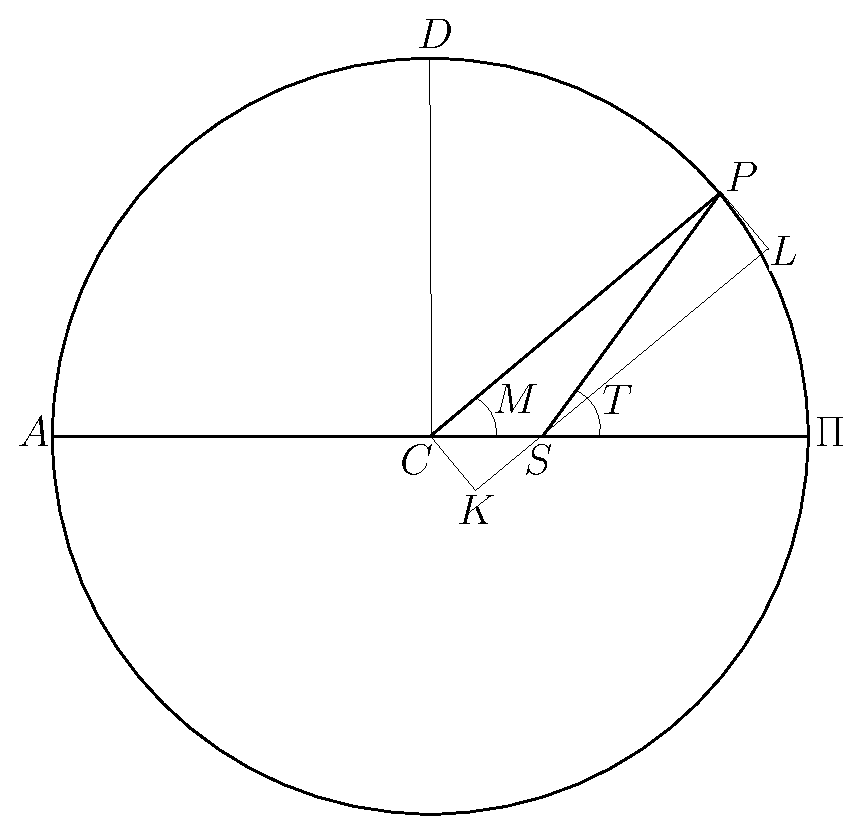
\includegraphics[height=2.5in]{Fig4-2.eps}}
\caption{A Hipparchian orbit.}\label{hipp}
\end{figure}

Let us draw the straight-line $KSL$ parallel to $CP$, and passing through point $S$, and then complete the rectangle $PCKL$. Simple geometry reveals that 
$CK = PL = 2\,e\,a\,\sin M$, $KS=2\,e\,a\,\cos M$, and  $SL = a-2\,e\,a\,\cos M$. Moreover, according to the theorem of Pythagoras, $SP^2 = SL^2+ PL^2$,
which implies that
\begin{equation}
\frac{r}{a} = (1-4\,e\,\cos M + 4\,e^2)^{1/2}.
\end{equation}
Now, $T = M + q$, where $q$ is angle $PSL$. However,
\begin{equation}
\sin q = \frac{PL}{SP} = \frac{2\,e\,\sin M}{(1-4\,e\,\cos M + 4\,e^2)^{1/2}}.
\end{equation}

Finally, expanding the previous two equations to second order in the small parameter $e$, we obtain
\begin{align}\label{e4.26}
\frac{r}{a} &= 1 -2\,e\,\cos M + 2\,e^2\,\sin^2 M,\\[0.5ex]
T &= M + 2\,e\,\sin M + 2\,e^2\,\sin 2M.\label{e4.27}
\end{align}
It can be seen, by comparison with Equations~(\ref{je22}) and (\ref{je23}), that   the relative radial distance, $r/a$, in the Hipparchian model deviates from that in the (correct) Keplerian model to  first order in $e$ (in fact, the variation of $r/a$
is greater by a factor of two in the former model), whereas 
 the true anomaly, $T$,  only deviates  to  second order  in $e$.  We conclude that  Hipparchus's geometric model
 of a heliocentric planetary orbit does a
 reasonably good job at predicting the angular position of the planet, relative to the Sun, but significantly
 exaggerates (by a factor of two) the variation in the radial distance between the two during the course of a complete  orbital rotation. 

\section{The model of Ptolemy}
Ptolemy's geometric model of the motion of the center of an epicycle around a deferent can also be used to describe a heliocentric planetary orbit. The model is illustrated  in Figure~\ref{ptol}. The orbit of the planet corresponds
to the circle $\Pi P D A$ (only half of which is shown), where $\Pi$ is the perihelion point, $P$ the planet's instantaneous position,
and $A$ the aphelion point. The diameter $\Pi   S C Q A$ is the effective major axis of the orbit, where $C$ is the geometric center of circle $\Pi P D A$,  $S$ the fixed position of the Sun, and $Q$  the location of the so-called {\em equant}.
The radius $CP$ of circle $\Pi PDA$ is   the effective major radius, $a$, of the orbit.  The distances $SC$ and $CQ$ are both
equal to $e\,a$, where $e$ is the orbit's effective eccentricity. The angle $PQ\Pi$
is  identified with the  mean anomaly, $M$, and increases linearly  in time.  In other words, as seen from $Q$, the planet
$P$ moves uniformly  around circle $\Pi PDA$ in a counterclockwise direction. Finally, $SP$ is the radial
distance, $r$, of the planet from the Sun, and angle $P S \Pi$ is the planet's true anomaly, $T$.

\begin{figure}[h]
\centerline{\includegraphics[height=2.5in]{Fig4-3.eps}}
\caption{A Ptolemaic orbit.}\label{ptol}
\end{figure}

Let us draw the straight-line $KSL$ parallel to $QP$, and passing through point $S$, and then complete the rectangle $PQKL$. Simple geometry reveals that 
$QK = PL = 2\,e\,a\,\sin M$, $KS=2\,e\,a\,\cos M$, and  $SL = \rho-2\,e\,a\,\cos M$, where
$\rho=QP$. The cosine rule applied to triangle $CQP$ yields
$CP^2 = CQ^2+QP^2-2\,CQ\,QP\,\cos M$, or $\rho^2-2\,e\,a\,\cos M\,\rho -a^2\,(1-e^2)=0$, which
can be solved to give $\rho/a = e\,\cos M +(1-e^2\,\sin^2 M)^{1/2}$. 
 Moreover, according to the theorem of Pythagoras,  $SP^2 = SL^2+ PL^2$,
which implies that
\begin{equation}\label{e4.30x}
\frac{r}{a} = [1-2\,e\,\cos M\,(1-e^2\,\sin^2 M)^{1/2}+e^2+2\,e^2\,\sin^2 M]^{1/2}.
\end{equation}
Now, $T = M + q$, where $q$ is angle $PSL$. However,
\begin{equation}\label{e4.31x}
\sin q = \frac{PL}{SP} = \frac{2\,e\,\sin M}{[1-2\,e\,\cos M\,(1-e^2\,\sin^2 M)^{1/2}+e^2+2\,e^2\,\sin^2 M]^{1/2}}.
\end{equation}

Finally, expanding the previous two equations to second order in the small parameter $e$, we obtain
\begin{align}
\frac{r}{a} &= 1 -e\,\cos M + (3/2)\,e^2\,\sin^2 M,\label{e4.30}\\[0.5ex]
T &= M + 2\,e\,\sin M + e^2\,\sin 2M.\label{e4.31}
\end{align}
It can be seen, by comparison with Equations~(\ref{je22})--(\ref{je23}) and (\ref{e4.26})--(\ref{e4.27}), that   Ptolemy's geometric model of a heliocentric planetary orbit is significantly
more accurate than  Hipparchus's model, because the 
relative radial distance, $r/a$,  and the true anomaly, $T$, in the former model both only deviate from those in the (correct) Keplerian model to second order in $e$.

\section{The model of Copernicus}
Copernicus's geometric model of  a heliocentric planetary orbit is illustrated  in Figure~\ref{cop}. 
The planet $P$ rotates on a circular epicycle $YP$ whose center $X$ moves around the Sun on the eccentric circle $\Pi X D A$ (only
half of which is shown). The diameter $\Pi S C A$ is the effective major axis of the orbit, where $C$ is the geometric center of circle $\Pi X D A$,  and $S$ the fixed position of the Sun. When $X$ is at  $\Pi$ or $A$ the planet is at its perihelion
or aphelion points, respectively.  The radius $CX$ of circle $\Pi XDA$ is   the effective major radius, $a$, of the orbit.  The distance $SC$ is
equal to $(3/2)\,e\,a$, where $e$ is the orbit's effective eccentricity. Moreover, the radius $XP$ of the epicycle is equal to $(1/2)\,e\,a$. 
The angle $XC\Pi$
is  identified with the  mean anomaly, $M$, and increases linearly   in time.  In other words, as seen from $C$, the center of
the epicycle
$X$ moves  uniformly  around circle $\Pi XDA$ in a counterclockwise direction. The angle $PXY$, where $Y$ is
point at which $CX$ produced meets the epicycle,  is equal to
the mean anomaly $M$. In other words, the planet $P$ moves  uniformly around the epicycle $YP$, in an counterclockwise direction, at  twice 
the speed that point $X$ moves around circle $\Pi XDA$.
 Finally, $SP$ is the radial
distance, $r$, of the planet from the Sun, and angle $P S \Pi$ is the planet's true anomaly, $T$.

\begin{figure}[h]
\centerline{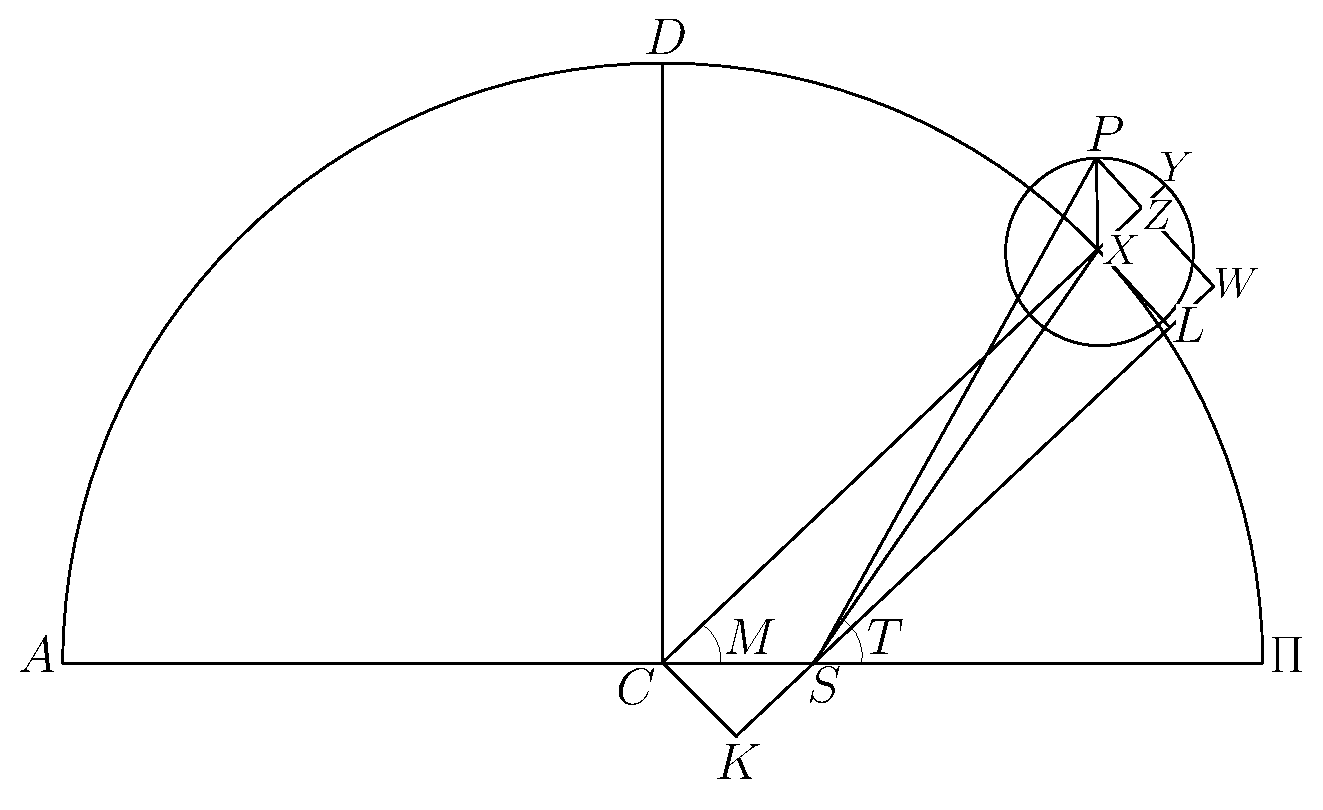
\includegraphics[height=2.5in]{Fig4-4.eps}}
\caption{A Copernican orbit.}\label{cop}
\end{figure}

Let us draw the straight-line $KSL$ parallel to $CX$, and passing through point $S$, and then complete the rectangle $XCKL$. Simple geometry reveals that 
$CK = XL = (3/2)\,e\,a\,\sin M$, $KS=(3/2)\,e\,a\,\cos M$, and  $SL = a-(3/2)\,e\,a\,\cos M$. Let $PZ$ be drawn normal
to $XY$, and let it meet $KSL$ produced at point $W$. Simple geometry reveals that $ZW=XL$,  $ZP=(1/2)\,e\,a\,\sin M$, and $XZ =LW = (1/2)\,e\,a\,\cos M$. It follows that $WP = ZW+ZP = XL+ZP = 2\,e\,a\,\sin M$, and $SW = SL+LW=SL+XZ= a-e\,a\,\cos\,M$.
Moreover, according to the theorem of Pythagoras,  $SP^2 = SW^2+ WP^2$,
which implies that
\begin{equation}
\frac{r}{a} = (1-2\,e\,\cos M +e^2+3\,e^2\,\sin^2 M)^{1/2}.
\end{equation}
Now, $T = M + q$, where $q$ is angle $PSW$. However,
\begin{equation}
\sin q = \frac{WP}{SP} = \frac{2\,e\,\sin M}{(1-2\,e\,\cos M +e^2+3\,e^2\,\sin^2 M)^{1/2}}.
\end{equation}

Finally, expanding the previous two equations to second order in the small parameter $e$, we obtain
\begin{align}
\frac{r}{a} &= 1 -e\,\cos M + 2\,e^2\,\sin^2 M,\\[0.5ex]
T &= M + 2\,e\,\sin M + e^2\,\sin 2M.
\end{align}
It can be seen, by comparison with Equations~(\ref{je22})--(\ref{je23}) and (\ref{e4.30})--(\ref{e4.31}), that, as is the case for Ptolemy's  model, both the 
relative radial distance, $r/a$,  and the true anomaly, $T$, in Copernicus's geometric model of a heliocentric planetary orbit only deviate from those in the (correct) Keplerian model to  second order  in $e$. However, the deviation  in the Ptolemaic
model is  slightly smaller  than that in the Copernican model. To be more exact, the maximum deviation in $r/a$
is $(1/2)\,e^2$ in the former model, and $e^2$ in the latter. On the other hand, the maximum deviation in $T$ is $(1/4)\,e^2$
in both models.
\chapter{The Sun}\label{csun}
% !TEX root = ./Almagest.tex

\section{Solar Ecliptic Longitude Model}
Our solar longitude model is sketched in Figure~\ref{lf3}. From a geocentric point of view, the Sun, $S$,  appears to execute
a (counterclockwise) Keplerian orbit of major radius $a$, and eccentricity $e$, about the
Earth, $G$. As has already been mentioned, the circle traced out by the Sun on the celestial sphere is
known as the  ecliptic circle. This circle is inclined at $23^\circ 26'$ to
the celestial equator, which is the projection of the Earth's equator onto
the celestial sphere.
 Suppose that the angle subtended at the Earth between the vernal equinox (that is, the point at which the ecliptic crosses the celestial equator from
south to north) and the
Sun's perigee (that is, the point of closest approach to the Earth)   is
 $\varpi$. This
angle is termed the {\em longitude of the perigee}, and
 is assumed
to vary  linearly with time: that is, 
\begin{equation}\label{ae79}
\varpi  = \varpi_0 + \varpi_1\,(t-t_0).
\end{equation}

\begin{figure}[h]
\centerline{\includegraphics[height=3in]{Fig5-1.eps}}
\caption{The apparent orbit of the Sun about the Earth.  Here, $S$, $G$, $\Pi$, $A$, $\varpi$, $T$,  $\lambda$, and $\Upsilon$
represent the Sun, the Earth, the perigee, the apogee, the longitude of the perigee, the true anomaly, the ecliptic longitude, and
The vernal equinox, respectively. the view is from northern ecliptic pole. The Sun orbits counterclockwise.}\label{lf3}
\end{figure}

 The Sun's {\em ecliptic
longitude}\/ is defined as the angle subtended at the Earth between the vernal equinox and the Sun.
Hence, from Figure~\ref{lf3},
\begin{equation}
\lambda = \varpi + T,
\end{equation}
where $T$ is the true anomaly. (See Chapter~\ref{ckep}.) By analogy, the  {\em mean longitude}\/ is written
\begin{equation}
\bar{\lambda} = \varpi + M,
\end{equation}
where $M$ is the  mean anomaly. (See Chapter~\ref{ckep}.) It follows from Equation~(\ref{je23}) that
\begin{equation}\label{ae82}
\lambda = \bar{\lambda}  + q,
\end{equation}
where
\begin{equation}
q = 2\,e\,\sin M + (5/4)\,e^2\,\sin\,2M,
\end{equation}
 is called  the {\em equation of  center}. Note that $\lambda$, $\bar{\lambda}$, $T$, and $M$ are usually written as angles in the range
 $0^\circ$ to $360^\circ$, whereas $q$ is generally written as an
 angle in the range $-180^\circ$ to $+180^\circ$. 

The mean longitude increases
uniformly with time (because both $\varpi$ and $M$ increase uniformly with time) as
\begin{equation}\label{ae84}
\bar{\lambda} =  \bar{\lambda}_0+ n\,(t -t_0),
\end{equation}
where $\bar{\lambda}_0$ is termed the
{\em mean longitude at epoch}, 
$n$ the {\em rate of motion in mean longitude}, and $t_0$ the {\em epoch}. 
We can also write
\begin{equation}\label{ae85}
M = M_0 + \tilde{n}\,(t-t_0),
\end{equation}
where
\begin{equation}
M_0 = \bar{\lambda}_0 - \varpi_0
\end{equation}
is called the {\em mean anomaly at epoch}, and 
\begin{equation}\label{ae87}
\tilde{n} = n - \varpi_1
\end{equation}
 the {\em rate of motion in mean anomaly}. 
 
 Our procedure for determining the ecliptic longitude of the Sun is as follows.
 The requisite orbital elements (that is, $e$, $n$, $\tilde{n}$, $\bar{\lambda}_0$, and $M_0$) for the J2000 epoch (that is, 12:00 UT on January 1, 2000 AD/, which corresponds to $t_0= 2\,451\,545.0$ JD) are listed
in Table~\ref{lt4}. These elements are calculated
on the assumption that the vernal equinox  precesses at the uniform
rate of $-3.8246\times 10^{-5}\,\,^\circ/{\rm day}$. 
The ecliptic longitude of the Sun is specified by the
following formulae:
\begin{align}
\bar{\lambda} &=  \bar{\lambda}_0+ n\,(t-t_0),\\[0.5ex]
M &= M_0 + \tilde{n}\,(t-t_0),\\[0.5ex]
q &= 2\,e\,\sin M + (5/4)\,e^2\,\sin\,2M,\label{le2.8}\\[0.5ex]
\lambda &= \bar{\lambda}  + q.
\end{align}
 These formulae are capable of matching NASA ephemeris data\,\footnote{See {\tt http://ssd.jpl.nasa.gov/}}
during the years 1995--2006 AD with a mean error of $0.2'$ and a maximum error of $0.7'$. 

The ecliptic longitude of the Sun can be calculated with the aid of Tables~\ref{lt5} and \ref{lt6}.
 Table~\ref{lt5} allows the mean longitude, $\bar{\lambda}$, and mean anomaly,
 $M$, of the
Sun to be determined as  functions of time. Table~\ref{lt6} specifies the equation of center, $q$, as a
function of the mean anomaly. 

 Note that Table~\ref{lt5} contains essentially the same information as that contained in the ``Table of the Sun's mean motion" (Κανόνιον τῆς ὁμαλῆς τοῦ ἡλίου κινήσεως) that appears in
 Section~2 of Book~III of the Almagest. Likewise, Table~\ref{lt6} contains essentially the same information as that contained in the ``Table of the solar anomaly'' (Κανόνιον τῆς  ἡλιακῆς ἀνωμαλίας)
 that appears in Section~6 of Book~III of the Almagest.
 
\section{Determination of Solar Ecliptic Longitude}\label{ssun}
The procedure for using Tables~\ref{lt5} and \ref{lt6} to determine solar longitude  is as follows:
\begin{enumerate}

\item Determine the fractional Julian day number, $t$, corresponding to the date and time
at which the Sun's ecliptic longitude is to be calculated with the aid of Tables~\ref{kt1}--\ref{kt3}. Form $\Delta t = t-t_0$, where $t_0=2\,451\,545.0$ is the epoch. 

\item Enter Table~\ref{lt5} with the digit for each power of 10
in ${\Delta} t$ and take out the corresponding values of $\Delta\bar{\lambda}$ and $\Delta M$. If $\Delta t$ is negative then the corresponding
values are also negative.
The value of the mean longitude, $\bar{\lambda}$, is the
sum of all the $\Delta\bar{\lambda}$ values plus the value of $\bar{\lambda}$ at the epoch. Likewise, the value of the mean anomaly, $M$, is
the sum of all the $\Delta M$ values plus the value of $M$ at the epoch. 
Add as many multiples of $360^\circ$ to $\bar{\lambda}$ and $M$
as is required to make them both fall in the range $0^\circ$ to $360^\circ$. Round $M$ to the nearest degree. 

\item Enter Table~\ref{lt6} with the value of $M$ and take out the
corresponding value of the equation of center, $q$, and the radial anomaly, $\zeta$. (The latter step is only necessary if the ecliptic longitude of the Sun is
to be used to determine that of a planet.) It is necessary to interpolate if $M$ is odd.

\item The ecliptic longitude, $\lambda$, is the sum of the mean longitude, $\bar{\lambda}$, and the equation of center, $q$. If necessary, convert $\lambda$ into an angle in the range $0^\circ$ to $360^\circ$. 
The decimal fraction can be converted into arc minutes
using Table~\ref{lt6a}. Round to the nearest arc minute. 
\end{enumerate}
Two examples of the use of this procedure are given in the next section.

\section{Example Solar Longitude Calculations}
\noindent {\em Example 1}: May 5, 2005 AD, 00:00 UT:\\
~\\
According to Tables~\ref{kt1}--\ref{kt3}, $t = 2\,453\,495.5$ JD. Hence,
$t-t_0 = 2\,453\,495.5-2\,451\,545.0=1\,950.5$ JD. Making use of
Table~\ref{lt5}, we find:\\
\begin{tabular}{rrr}
&&\\
$t$(JD) & $ \bar{\lambda}(^\circ)$ & $M(^\circ)$\\[-2ex]
&&\\
$+1\,000$ & $265.647$ & $265.600$\\
$+900$ & $167.083$ & $167.040$\\
$+50$ & $49.282$ & $49.280$\\
$+.5$ & $0.493$ & $0.493$\\
Epoch & $280.458$ & $357.588$\\\cline{2-3}
&$762.963$ & $840.001$\\\cline{2-3}
Modulus & $42.963$ & $120.001$\\ 
&&\\
\end{tabular}\\
Rounding the mean anomaly to the nearest degree, we obtain $M\simeq 120^\circ$.
It follows from  Table~\ref{lt6} that
$$
q(120^\circ)= 1.641^\circ,
$$ 
so
$$
\lambda =\bar{\lambda} + q =42.961+ 1.641=44.602\simeq 44^\circ36'.
$$
Here, we have converted the decimal fraction into arc
minutes using Table~\ref{lt6a}, and 
then rounded the final result to the nearest arc minute.

 Following
the practice of the Ancient Greeks (and modern-day astrologers), we shall express ecliptic longitudes
in terms of the  signs of the zodiac, which  are listed in Section~\ref{szod}. The ecliptic longitude $44^\circ36'$ is conventionally written 14TA36;  that is, 
$14^\circ36'$ into the sign of Taurus. Thus, we conclude that the position of
the Sun 
at 00:00 UT on May 5, 2005 AD was 14TA36.

~\\
\noindent {\em Example 2}: December 25, 1800 AD, 00:00 UT:\\
~\\
According to Tables~\ref{kt1}--\ref{kt3}, $t = 2\,378\,854.5$ JD. Hence,
$ t-t_0 = 2\,378\,854.5-2\,451\,545.0=-72\,690.5$ JD. Making use of
Table~\ref{lt5}, we find:\\
\begin{tabular}{rrr}
&&\\
$t$(JD) & $\bar{\lambda}(^\circ)$ & $ M(^\circ)$\\[-2ex]
&&\\
$-70\,000 $& $-235.315$ & $-232.017$\\
$-2\,000$ & $-171.295$ & $-171.200$\\
$-600$ & $-231.388$ & $-231.360$\\
$-90$ & $-88.708$ & $-88.704$\\
$-.5$ & $-0.493$ & $-0.493$\\
Epoch & $280.458$ & $357.588$\\\cline{2-3}
&$-446.741$ & $-366.186$\\\cline{2-3}
Modulus & $273.259$ & $353.814$\\
&&\\
\end{tabular}\\
We conclude that  $M\simeq 354^\circ$. 
 From Table~\ref{lt6}, 
$$
q(354^\circ)= -0.204^\circ,
$$  
so
$$
\lambda =\bar{\lambda} + q = 273.259 - 0.204=273.055\simeq 273^\circ03'.
$$
 Thus, the position of the Sun at 00:00 UT on December 25, 1800 AD was 3CP03. 
 
\section{Determination of Equinox and Solstice Dates}
We can also use Tables~\ref{lt5} and \ref{lt6} to calculate the dates of the equinoxes and solstices,
and, hence, the lengths of the seasons, in a given year. The {\em vernal equinox}\/ (that is, the point on the Sun's apparent orbit at which it passes through the celestial equator
from south to north)
corresponds to $\lambda=0^\circ$, the {\em summer solstice}\/ (that is, the
point at which the Sun is farthest north of the celestial equator) to $\lambda=90^\circ$, the {\em autumnal equinox}\/ (that is, the point at which the
Sun passes through the celestial equator from north to south) to $\lambda = 180^\circ$, and the
{\em winter solstice}\/ (that is, the point at which the Sun is farthest south of the celestial equator) to $\lambda = 270^\circ$. See Figure~\ref{lf6a}. Furthermore, {\em spring}\/ is defined as the period between the spring
equinox and the summer solstice, {\em summer}\/ as the period between the summer solstice and
the autumnal equinox, {\em autumn}\/ as the period between the autumnal equinox and the
winter solstice, and {\em winter}\/ as the period between the winter solstice and the following
vernal equinox. Consider the year 2000 AD.
For the case of the vernal equinox, we can
 first estimate the
 time at which this event takes place by approximating the solar
 longitude as the  mean
solar longitude; that is, 
$$
\lambda\simeq \bar{\lambda} = \bar{\lambda}_0 + n\,(t-t_0)
= 280.458 +  0.98564735\,(t-t_0),
$$
 We obtain 
$$
t \simeq t_0+(360-280.458)/0.98564735 \simeq t_0+81\,{\rm JD}.
$$ 
Calculating the true solar longitude at this time, using Tables~\ref{lt5} and \ref{lt6}, we get  
$\lambda = 2.177^\circ.$ Now, the actual vernal equinox occurs
when $\lambda=0^\circ$.
Thus, a much better estimate for the date of the vernal equinox
is
$$
t = t_0 + 81 -2.177/0.98564735 \simeq t_0 + 78.8\,{\rm JD},
$$
 which
corresponds to 7:00 UT on March 20. Similar calculations show that the summer solstice takes place at 
$$
t = t_0+ 171.6\, {\rm JD},
$$
corresponding to 2:00 UT on June 21, that the autumnal equinox
takes place at 
$$
t = t_0+265.2\,{\rm JD},
$$
corresponding to 17:00 UT
on September 22, and that the winter solstice takes place at
$$
t =t_0+355.1\, {\rm JD},
$$
corresponding to 14:00 UT on December 21. 
Thus, the length of spring is $92.8$ days,
the length of summer $93.6$ days,
and the length of autumn  $89.9$ days.
Finally, the length of winter is the length
of the tropical year (that is, the time period between successive vernal equinoxes), which is $360/0.98564735 = 325.24$ days, minus the sum of the lengths of the
other three seasons. This gives $88.9$ days. 

\begin{figure}[t]
\centerline{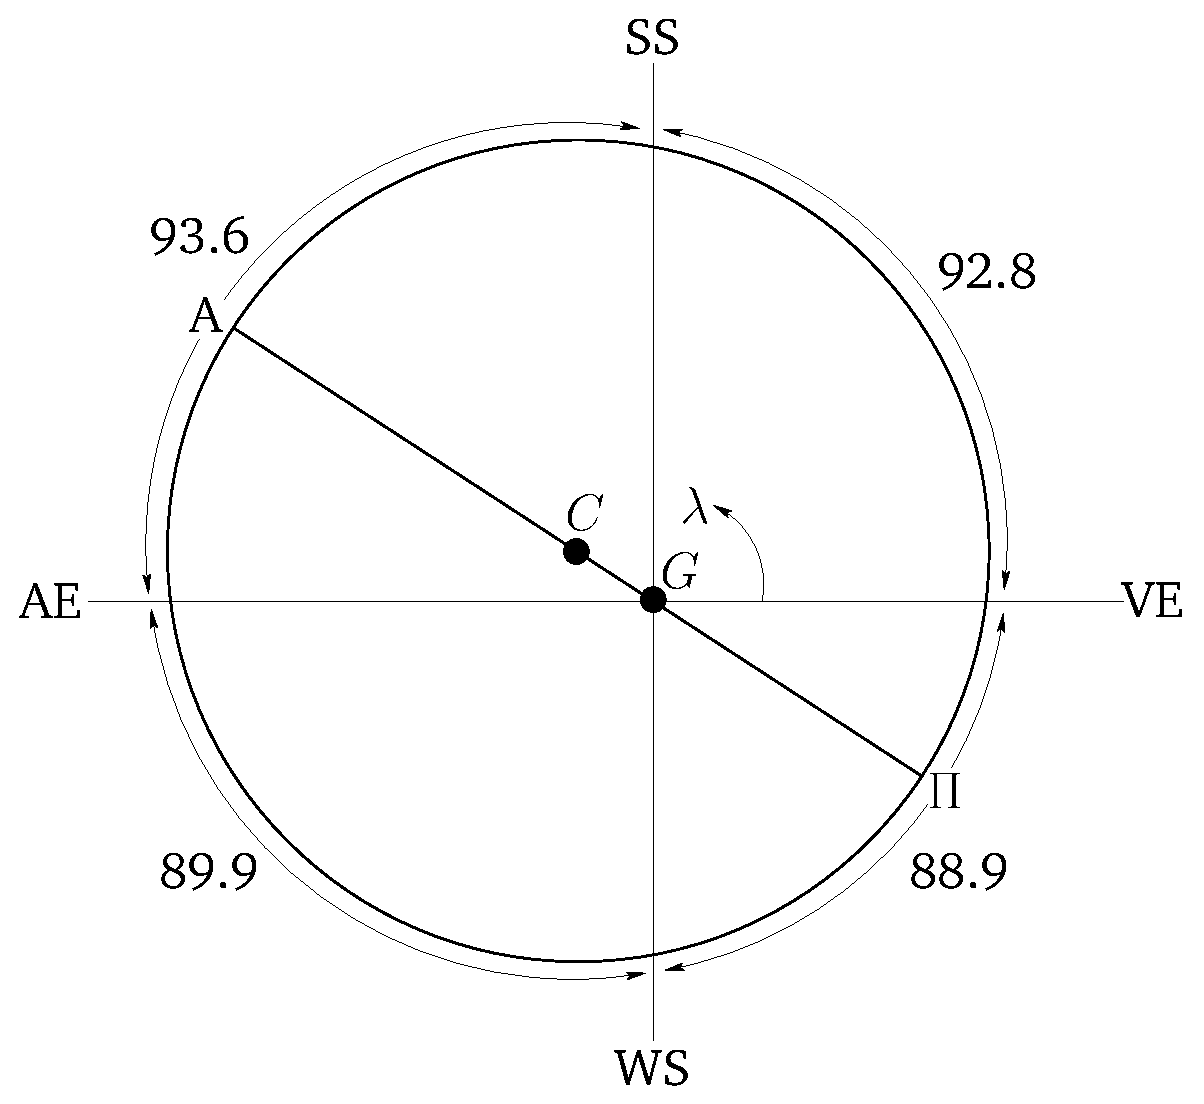
\includegraphics[height=3.5in]{Fig5-2.eps}}
\caption{The Sun's apparent orbit around the Earth, $G$, showing the vernal equinox (VE), summer
solstice (SS), autumnal equinox (AE), and winter solstice (WS). Here, $\lambda$, $\Pi$, $A$, and $C$
are the ecliptic longitude, the perigee, the apogee, and the geometric center of the orbit, respectively. The lengths
of the seasons (in days) are  indicated. }\label{lf6a}   
\end{figure}

Figure~\ref{lf6a} illustrates the relationship between the equinox and solstice points, and the
lengths of the seasons. The Earth is displaced from the geometric center of the Sun's apparent orbit in the direction of
the solar perigee, which presently lies between the winter solstice and the vernal equinox. This displacement (which is
greatly exaggerated in the figure) has
two effects. Firstly, it causes the arc of the Sun's apparent orbit between the summer solstice and autumnal equinox
to be longer than that between the winter solstice and the vernal equinox. Secondly, it causes the
Sun to appear to move faster in winter than in summer, in accordance with Kepler's second law, because the Sun is closer to the Earth in the
former season. Both of these effects tend to lengthen summer, and
shorten winter. Hence, summer is presently the longest season, and winter the shortest.

In Section~4 of Book~III of the Almagest, Ptolemy effectively performs the calculation described in this section in reverse, in order to determine the eccentricity of the Sun's
apparent orbit about the Earth, as well as the location of the solar perigee,  from the observed differences in the lengths of the seasons. However, Ptolemy's figures for the lengths of spring, summer, autumn, and winter,
which he inherited from Hipparchus,  were
94.5, 92.5, 88.125, and 90.125 days, respectively. The lengths of the seasons have changed since the time of Hipparchus because the solar perigee has
rotated by about $38^\circ$ (in the direction of the Sun's apparent motion) over the last 2\,200 years. 

\section{Equation of Time}
At any particular observation site on the Earth's surface, {\em local noon}\/
is defined as the instant in time when the Sun culminates at the
meridian. However, as a consequence of the inclination of the
ecliptic to the celestial equator, as well as the uneven motion of the
Sun around the ecliptic, the time interval  between successive local noons, which
is known as a {\em solar day}, 
is not constant, but varies throughout the year. Hence, if we were to
define a second as $1/86\,400$ of a solar day then the length of a second
would also vary throughout the year, which is clearly undesirable. In
order to avoid this problem, astronomers have invented a fictitious
body called the {\em mean Sun}. The mean Sun travels around the
celestial equator (from west to east) at a constant
rate that is such that it completes one orbit every tropical year. Moreover,
the mean Sun and the true Sun coincide at the spring equinox. {\em Local mean noon}\/ at a particular observation
site is defined as the instance in time when the mean Sun culminates at
the meridian. Because the orbit of the mean Sun is not inclined to the
celestial equator, and the mean Sun travels  around the celestial equator at a uniform rate, the time
interval between successive mean noons, which is known as a
{\em mean solar day}, takes the constant value of 24 hours, or
86\,400 seconds, throughout the year. {\em Universal time}\/ (UT)
is defined such that 12:00  UT coincides with mean noon every day at
an observation site of terrestrial longitude $0^\circ$. If we define {\em local  time}\/
(LT)
as $LT = UT- \phi(^\circ)/15^\circ$ hrs., where $\phi$ is the terrestrial longitude
of the observation site, then 12:00  LT coincides with mean noon
every day at a general observation site on the Earth's surface.

According to the previous definition, the right ascension, $\bar{\alpha}$, of the mean
Sun satisfies
\begin{equation}
\bar{\alpha} = \bar{\lambda},
\end{equation}
where $\bar{\lambda}$ is the Sun's mean ecliptic longitude. Moreover,
it follows from Equations~(\ref{e15r})  and (\ref{ae82}) that the right ascension
of the true Sun is given by
\begin{equation}
\tan\alpha = \cos\epsilon\,\tan(\bar{\lambda}+q),
\end{equation}
where $\epsilon$ is the inclination of the ecliptic to the celestial
equator, $q(M)$  the Sun's equation of center, and $M$ its mean anomaly. Now, neglecting the small time variation of the longitude of the
Sun's perigee [that is, setting $\varpi_1=0$ in Equation~(\ref{ae79})], we 
can write [see Equations~(\ref{ae84}), (\ref{ae85}), and (\ref{ae87}), as
well as Table~\ref{lt4}]
\begin{equation}
M = \bar{\lambda} + M_0-\bar{\lambda}_0 = \bar{\lambda} +77.213^\circ.
\end{equation}
It follows that, to first order in the solar eccentricity, $e$, we have
\begin{equation}
\Delta\alpha = \bar{\alpha}-\alpha = \lambda - \tan^{-1}(\cos \epsilon\,\tan\lambda) - 2\,e\,\sin\,M,
\end{equation}
where
\begin{equation}
M = \lambda + 77.213^\circ.
\end{equation}
Now,
\begin{equation}
\Delta t = \Delta\alpha(^\circ)/15^\circ
\end{equation}
represents the time difference (in hours) between local noon and mean local noon (because
right ascension crosses the meridian at the uniform rate of $15^\circ$ an
hour), and  is known as the {\em equation of time}. If $\Delta t$ is
positive then local noon occurs before mean local noon, and  vice
versa. 

The equation of time specifies the difference between  time calculated using a sundial or sextant---which is known as
{\em solar time}---and
time obtained from  an accurate clock---which is known as {\em mean solar time}. Table~\ref{ttime} shows the equation of time as a function of the Sun's
ecliptic longitude. It can be seen that the difference between solar time and mean solar time can be as much as
16 minutes, and attains its maximum value between the autumnal equinox and the winter solstice, and its
minimum value between the winter solstice and vernal equinox.

The equation of time is discussed in Section~9 of Book~III of the Almagest. 

\section{Solar Distance Model}
The distance, $r$,  of the Sun from the Earth varies slightly over the course of a year because the Earth is not quite at the geometric center of the Sun's apparent orbit. 
It follows that the apparent angular size of the solar disk in the Earth's sky also exhibits an annual variation. We need to understand this variation in order to
accurately predict lunar and solar eclipses. 
According to Equation~(\ref{je22}), 
\begin{equation}\label{e5.20j}
\frac{r}{a} = 1 -\zeta
\end{equation}
where
\begin{equation}
\zeta = e\,\cos\,M -e^{\,2}\,\sin^2\,M.
\end{equation}
Here, $a=1.498\times 10^8$ km is the Sun's (apparent) orbital major radius, and $\zeta$ is known as a {\em radial anomaly}. The solar radial anomaly
is tabulated as a function of its argument ($M$) in Table~\ref{lt6}. 

The apparent radius of the solar disk is
\begin{equation}\label{e5.22j}
\rho_S = \frac{R}{r},
\end{equation}
where $R= 6.957\times 10^5$\,km is the mean physical radius of the Sun. Here, use has been made of the small angle approximation.
It follows  from Equations~(\ref{e5.20j}) and (\ref{e5.22j}) that
\begin{equation}\label{rhos}
\rho_S = \frac{15.987'}{1-\zeta}.
\end{equation}
Clearly, the mean diameter of the solar disk is about half a degree. 

As an example of a solar apparent radius calculation, we have already seen that at 00:00 UT on May 5, 2005 AD the  mean anomaly of the Sun was
$M\simeq 120^\circ$. It follows from Table~\ref{lt6} that the solar radial anomaly was $\zeta=-0.856\times 10^{-2}$. Hence, the
apparent radius of the solar disk was
\begin{equation}
\rho_S = \frac{15.987}{1+0.856\times 10^{-2}}\simeq 15.85'.
\end{equation}

As a second example of a solar radius calculation, we have also seen that at 00:00 UT on December 25, 1800 AD the mean anomaly
of the Sun was $M\simeq 354^\circ$. It follows from Table~\ref{lt6} that the solar radial anomaly was $\zeta=1.662\times 10^{-2}$. 
Hence, the
apparent radius of the solar disk was
\begin{equation}
\rho_S = \frac{15.987}{1-1.662\times 10^{-2}}\simeq 16.26'.
\end{equation}

\section{Tables}

\begin{table}[b]\centering
\begin{tabular}{l|rcrrrr}
Object &  $a\,({\rm AU})$ & $e$ & $n\,(^\circ/{\rm day})$ & $\tilde{n}\,(^\circ/{\rm day})$ & $\bar{\lambda}_0\,(^\circ)$ & $M_0\,(^\circ)$\\\hline
&&&&&&\\[-2.2ex]
Mercury & $0.387098$  & $0.205636$ & $4.09237703$     & $4.09233439$    & $252.087$ & $174.693$  \\
Venus     & $0.723334$  & $0.006777$  & $1.60216872$    & $1.60213040$  & $181.973$ & $49.237$ \\
Sun       & $1.000000$  & $0.016711$  & $0.98564735$      & $0.98560025$  & $280.458$ & $357.588$   \\
Mars      & $1.523706$  & $0.093394$  & $0.52407118$     & $0.52402076$  & $355.460$ & $19.388$ \\ 
Jupiter   & $5.202873$  & $0.048386$  & $0.08312507$     & $0.08308100$    & $34.365$ & $19.348$\\
Saturn   & $9.536651$  & $0.053862$    & $0.03350830$     & $0.03348152$   & $50.059$ & $317.857$ \\
\end{tabular}
\caption{Keplerian orbital elements for the Sun and the five visible planets at the J2000 epoch (that is, 12:00 UT, January 1, 2000 AD,
which corresponds to $t_0 = 2\,451\,545.0$ JD). The elements are optimized for use in the
time period 1800 AD to 2050 AD. Source: Jet Propulsion Laboratory (NASA), {\tt http://ssd.jpl.nasa.gov/}.  The motion rates have been converted into tropical motion rates assuming a uniform precession of the equinoxes
 of $3.8246\times 10^{-5}\,\,^\circ$ per day. An astronomical unit (AU) is $1.496\times 10^8$\,km.}\label{lt4}
\end{table}

\clearpage
\begin{table}\centering
{\small\begin{tabular}{ll|ll|ll|ll|ll|ll}
$00.0'$ & .000 & $10.0'$ & .167 & $20.0'$ & .333 & $30.0'$ & .500 & $40.0'$ & .667 & $50.0'$ & .833\\
$00.2'$ & .003 & $10.2'$ & .170 & $20.2'$ & .337 & $30.2'$ & .503 & $40.2'$ & .670 & $50.2'$ & .837\\
$00.4'$ & .007 & $10.4'$ & .173 & $20.4'$ & .340 & $30.4'$ & .507 & $40.4'$ & .673 & $50.4'$ & .840\\
$00.6'$ & .010 & $10.6'$ & .177 & $20.6'$ & .343 & $30.6'$ & .510 & $40.6'$ & .677 & $50.6'$ & .843\\
$00.8'$ & .013 & $10.8'$ & .180 & $20.8'$ & .347 & $30.8'$ & .513 & $40.8'$ & .680 & $50.8'$ & .847\\
$01.0'$ & .017 & $11.0'$ & .183 & $21.0'$ & .350 & $31.0'$ & .517 & $41.0'$ & .683 & $51.0'$ & .850\\
$01.2'$ & .020 & $11.2'$ & .187 & $21.2'$ & .353 & $31.2'$ & .520 & $41.2'$ & .687 & $51.2'$ & .853\\
$01.4'$ & .023 & $11.4'$ & .190 & $21.4'$ & .357 & $31.4'$ & .523 & $41.4'$ & .690 & $51.4'$ & .857\\
$01.6'$ & .027 & $11.6'$ & .193 & $21.6'$ & .360 & $31.6'$ & .527 & $41.6'$ & .693 & $51.6'$ & .860\\
$01.8'$ & .030 & $11.8'$ & .197 & $21.8'$ & .363 & $31.8'$ & .530 & $41.8'$ & .697 & $51.8'$ & .863\\
$02.0'$ & .033 & $12.0'$ & .200 & $22.0'$ & .367 & $32.0'$ & .533 & $42.0'$ & .700 & $52.0'$ & .867\\
$02.2'$ & .037 & $12.2'$ & .203 & $22.2'$ & .370 & $32.2'$ & .537 & $42.2'$ & .703 & $52.2'$ & .870\\
$02.4'$ & .040 & $12.4'$ & .207 & $22.4'$ & .373 & $32.4'$ & .540 & $42.4'$ & .707 & $52.4'$ & .873\\
$02.6'$ & .043 & $12.6'$ & .210 & $22.6'$ & .377 & $32.6'$ & .543 & $42.6'$ & .710 & $52.6'$ & .877\\
$02.8'$ & .047 & $12.8'$ & .213 & $22.8'$ & .380 & $32.8'$ & .547 & $42.8'$ & .713 & $52.8'$ & .880\\
$03.0'$ & .050 & $13.0'$ & .217 & $23.0'$ & .383 & $33.0'$ & .550 & $43.0'$ & .717 & $53.0'$ & .883\\
$03.2'$ & .053 & $13.2'$ & .220 & $23.2'$ & .387 & $33.2'$ & .553 & $43.2'$ & .720 & $53.2'$ & .887\\
$03.4'$ & .057 & $13.4'$ & .223 & $23.4'$ & .390 & $33.4'$ & .557 & $43.4'$ & .723 & $53.4'$ & .890\\
$03.6'$ & .060 & $13.6'$ & .227 & $23.6'$ & .393 & $33.6'$ & .560 & $43.6'$ & .727 & $53.6'$ & .893\\
$03.8'$ & .063 & $13.8'$ & .230 & $23.8'$ & .397 & $33.8'$ & .563 & $43.8'$ & .730 & $53.8'$ & .897\\
$04.0'$ & .067 & $14.0'$ & .233 & $24.0'$ & .400 & $34.0'$ & .567 & $44.0'$ & .733 & $54.0'$ & .900\\
$04.2'$ & .070 & $14.2'$ & .237 & $24.2'$ & .403 & $34.2'$ & .570 & $44.2'$ & .737 & $54.2'$ & .903\\
$04.4'$ & .073 & $14.4'$ & .240 & $24.4'$ & .407 & $34.4'$ & .573 & $44.4'$ & .740 & $54.4'$ & .907\\
$04.6'$ & .077 & $14.6'$ & .243 & $24.6'$ & .410 & $34.6'$ & .577 & $44.6'$ & .743 & $54.6'$ & .910\\
$04.8'$ & .080 & $14.8'$ & .247 & $24.8'$ & .413 & $34.8'$ & .580 & $44.8'$ & .747 & $54.8'$ & .913\\
$05.0'$ & .083 & $15.0'$ & .250 & $25.0'$ & .417 & $35.0'$ & .583 & $45.0'$ & .750 & $55.0'$ & .917\\
$05.2'$ & .087 & $15.2'$ & .253 & $25.2'$ & .420 & $35.2'$ & .587 & $45.2'$ & .753 & $55.2'$ & .920\\
$05.4'$ & .090 & $15.4'$ & .257 & $25.4'$ & .423 & $35.4'$ & .590 & $45.4'$ & .757 & $55.4'$ & .923\\
$05.6'$ & .093 & $15.6'$ & .260 & $25.6'$ & .427 & $35.6'$ & .593 & $45.6'$ & .760 & $55.6'$ & .927\\
$05.8'$ & .097 & $15.8'$ & .263 & $25.8'$ & .430 & $35.8'$ & .597 & $45.8'$ & .763 & $55.8'$ & .930\\
$06.0'$ & .100 & $16.0'$ & .267 & $26.0'$ & .433 & $36.0'$ & .600 & $46.0'$ & .767 & $56.0'$ & .933\\
$06.2'$ & .103 & $16.2'$ & .270 & $26.2'$ & .437 & $36.2'$ & .603 & $46.2'$ & .770 & $56.2'$ & .937\\
$06.4'$ & .107 & $16.4'$ & .273 & $26.4'$ & .440 & $36.4'$ & .607 & $46.4'$ & .773 & $56.4'$ & .940\\
$06.6'$ & .110 & $16.6'$ & .277 & $26.6'$ & .443 & $36.6'$ & .610 & $46.6'$ & .777 & $56.6'$ & .943\\
$06.8'$ & .113 & $16.8'$ & .280 & $26.8'$ & .447 & $36.8'$ & .613 & $46.8'$ & .780 & $56.8'$ & .947\\
$07.0'$ & .117 & $17.0'$ & .283 & $27.0'$ & .450 & $37.0'$ & .617 & $47.0'$ & .783 & $57.0'$ & .950\\
$07.2'$ & .120 & $17.2'$ & .287 & $27.2'$ & .453 & $37.2'$ & .620 & $47.2'$ & .787 & $57.2'$ & .953\\
$07.4'$ & .123 & $17.4'$ & .290 & $27.4'$ & .457 & $37.4'$ & .623 & $47.4'$ & .790 & $57.4'$ & .957\\
$07.6'$ & .127 & $17.6'$ & .293 & $27.6'$ & .460 & $37.6'$ & .627 & $47.6'$ & .793 & $57.6'$ & .960\\
$07.8'$ & .130 & $17.8'$ & .297 & $27.8'$ & .463 & $37.8'$ & .630 & $47.8'$ & .797 & $57.8'$ & .963\\
$08.0'$ & .133 & $18.0'$ & .300 & $28.0'$ & .467 & $38.0'$ & .633 & $48.0'$ & .800 & $58.0'$ & .967\\
$08.2'$ & .137 & $18.2'$ & .303 & $28.2'$ & .470 & $38.2'$ & .637 & $48.2'$ & .803 & $58.2'$ & .970\\
$08.4'$ & .140 & $18.4'$ & .307 & $28.4'$ & .473 & $38.4'$ & .640 & $48.4'$ & .807 & $58.4'$ & .973\\
$08.6'$ & .143 & $18.6'$ & .310 & $28.6'$ & .477 & $38.6'$ & .643 & $48.6'$ & .810 & $58.6'$ & .977\\
$08.8'$ & .147 & $18.8'$ & .313 & $28.8'$ & .480 & $38.8'$ & .647 & $48.8'$ & .813 & $58.8'$ & .980\\
$09.0'$ & .150 & $19.0'$ & .317 & $29.0'$ & .483 & $39.0'$ & .650 & $49.0'$ & .817 & $59.0'$ & .983\\
$09.2'$ & .153 & $19.2'$ & .320 & $29.2'$ & .487 & $39.2'$ & .653 & $49.2'$ & .820 & $59.2'$ & .987\\
$09.4'$ & .157 & $19.4'$ & .323 & $29.4'$ & .490 & $39.4'$ & .657 & $49.4'$ & .823 & $59.4'$ & .990\\
$09.6'$ & .160 & $19.6'$ & .327 & $29.6'$ & .493 & $39.6'$ & .660 & $49.6'$ & .827 & $59.6'$ & .993\\
$09.8'$ & .163 & $19.8'$ & .330 & $29.8'$ & .497 & $39.8'$ & .663 & $49.8'$ & .830 & $59.8'$ & .997\\
\end{tabular}}
\caption{Arc minute to decimal fraction conversion table.}\label{lt6a}
\end{table}

\newpage
\begin{table}[h]
\centering
\begin{tabular}{rrr|rrr|rrr}
$\Delta t$(JD)& $\Delta\bar{\lambda}(^\circ)$ &  $\Delta M(^\circ)$ & $\Delta t$(JD)& $\Delta \bar{\lambda}(^\circ)$ & $\Delta M(^\circ)$ &$\Delta t$(JD)& $\Delta \bar{\lambda}(^\circ)$ & $\Delta M(^\circ)$\\ \hline
&&&&&&&&\\[-1.75ex]
$10\,000$ & $136.474$ & $136.002$ & $1\,000$ & $265.647$ & $265.600$& $100$ &  $98.565$ &  $98.560$\\
$20\,000$ & $272.947$ & $272.005$ & $2\,000$ & $171.295$ & $171.200$ & $200$ & $197.129$ & $197.120$\\
$30\,000$ &  $49.421$ &  $48.007$ & $3\,000$ &  $76.942$ &  $76.801$ & $300$ & $295.694$ & $295.680$\\
$40\,000$ & $185.894$ & $184.010$ & $4\,000$ & $342.589$ & $342.401$ & $400$ &  $34.259$ &  $34.240$\\
$50\,000$ & $322.367$ & $320.012$ & $5\,000$ & $248.237$ & $248.001$ & $500$ & $132.824$ & $132.800$\\
$60\,000$ &  $98.841$ &  $96.015$ & $6\,000$ & $153.884$ & $153.601$ & $600$ & $231.388$ & $231.360$\\
$70\,000$ & $235.315$ & $232.017$ & $7\,000$ &  $59.531$ &  $59.202$ & $700$ & $329.953$ & $329.920$\\
$80\,000$ &  $11.788$ &   $8.020$ & $8\,000$ & $325.179$ & $324.802$ & $800$ &  $68.518$ &  $68.480$\\
$90\,000$ & $148.262$ & $144.022$ & $9\,000$ & $230.826$ & $230.402$ & $900$ & $167.083$ & $167.040$\\
&&&&&&&&\\
$10$ &   $9.856$ &   $9.856$ & $1$ &   $0.986$ &   $0.986$ & $0.1$ &   $0.099$ &   $0.099$\\
$20$ &  $19.713$ &  $19.712$ & $2$ &   $1.971$ &   $1.971$ & $0.2$ &   $0.197$ &   $0.197$\\
$30$ &  $29.569$ &  $29.568$ & $3$ &   $2.957$ &   $2.957$ & $0.3$ &   $0.296$ &   $0.296$\\
$40$ &  $39.426$ &  $39.424$ & $4$ &   $3.943$ &   $3.942$ & $0.4$ &   $0.394$ &   $0.394$\\
$50$ &  $49.282$ &  $49.280$ & $5$ &   $4.928$ &   $4.928$ & $0.5$ &   $0.493$ &   $0.493$\\
$60$ &  $59.139$ &  $59.136$ & $6$ &   $5.914$ &   $5.914$ & $0.6$ &   $0.591$ &   $0.591$\\
$70$ &  $68.995$ &  $68.992$ & $7$ &   $6.900$ &   $6.899$ & $0.7$ &   $0.690$ &   $0.690$\\
$80$ &  $78.852$ &  $78.848$ & $8$ &   $7.885$ &   $7.885$ & $0.8$ &   $0.789$ &   $0.788$\\
$90$ &  $88.708$ &  $88.704$ & $9$ &   $8.871$ &   $8.870$ & $0.9$ &   $0.887$ &   $0.887$\\
\end{tabular}
\caption{Mean motion of the Sun.  Here, $\Delta t = t-t_0$, $\Delta\bar{\lambda} = \bar{\lambda}-\bar{\lambda}_0$, and $\Delta M = M - M_0$. 
At epoch  ($t_0 = 2\,451\,545.0$ JD), $\bar{\lambda}_0 = 280.458^\circ$, and $M_0 = 357.588^\circ$.}\label{lt5}
\end{table}

\newpage
\begin{table}\centering
\small{ \begin{tabular}{rrr|rrr|rrr|rrr}
$M(^\circ)$ & $q(^\circ)$  & $100\,\zeta$ & $M(^\circ)$ & $q(^\circ)$  & $100\,\zeta$ & $M(^\circ)$ & $q(^\circ)$  & $100\,\zeta$& $M(^\circ)$ & $q(^\circ)$  & $100\,\zeta$\\\hline
&&&&&&&&&&&\\[-1.75ex]
  $0$ &  $0.000$ &  $1.671$ &  $90$ &  $1.915$ & $-0.028$ & $180$ &  $0.000$ & $-1.671$ & $270$ & $-1.915$ & $-0.028$\\
  $2$ &  $0.068$ &  $1.670$ &  $92$ &  $1.912$ & $-0.086$ & $182$ & $-0.065$ & $-1.670$ & $272$ & $-1.915$ & $0.030$\\
  $4$ &  $0.136$ &  $1.667$ &  $94$ &  $1.907$ & $-0.144$ & $184$ & $-0.131$ & $-1.667$ & $274$ & $-1.913$ &  $0.089$\\
  $6$ &  $0.204$ &  $1.662$ &  $96$ &  $1.900$ & $-0.202$ & $186$ & $-0.196$ & $-1.662$ & $276$ & $-1.909$ &  $0.147$\\
  $8$ &  $0.272$ &  $1.654$ &  $98$ &  $1.891$ & $-0.260$ & $188$ & $-0.261$ & $-1.655$ & $278$ & $-1.902$ &  $0.205$\\
 $10$ & $0.339$ &  $1.645$ & $100$ &  $1.879$ & $-0.317$ & $190$ & $-0.326$ & $-1.647$ & $280$ & $-1.893$ &  $0.263$\\
 $12$ &  $0.406$ &  $1.633$ & $102$ &  $1.865$ & $-0.374$ & $192$ & $-0.390$ & $-1.636$ & $282$ & $-1.881$ &  $0.321$\\
 $14$ &  $0.473$ &  $1.620$ & $104$ &  $1.849$ & $-0.431$ & $194$ & $-0.454$ & $-1.623$ & $284$ & $-1.867$ &  $0.378$\\
 $16$ &  $0.538$ &  $1.604$ & $106$ &  $1.830$ & $-0.486$ & $196$ & $-0.517$ & $-1.608$ & $286$ & $-1.851$ &  $0.435$\\
 $18$ &  $0.604$ &  $1.587$ & $108$ &  $1.809$ & $-0.542$ & $198$ & $-0.580$ & $-1.592$ & $288$ & $-1.833$ &  $0.491$\\
 $20$ &  $0.668$ &  $1.567$ & $110$ &  $1.787$ & $-0.596$& $200$ & $-0.642$ & $-1.574$ & $290$ & $-1.812$ &  $0.547$\\
 $22$ &  $0.731$ &  $1.545$ & $112$ &  $1.762$ & $-0.650$ & $202$ & $-0.703$ & $-1.553$ & $292$ & $-1.789$ &  $0.602$\\
 $24$ &  $0.794$ &  $1.522$ & $114$ &  $1.735$ & $-0.703$ & $204$ & $-0.764$ & $-1.531$ & $294$ & $-1.764$ &  $0.656$\\
 $26$ &  $0.855$ &  $1.497$ & $116$ &  $1.705$ & $-0.755$ & $206$ & $-0.824$ & $-1.507$ & $296$ & $-1.737$ &  $0.710$\\
 $28$ &  $0.916$ &  $1.469$ & $118$ &  $1.674$ & $-0.806$ & $208$ & $-0.882$ & $-1.482$ & $298$ & $-1.707$ &  $0.763$\\
 $30$ &  $0.975$ &  $1.440$ & $120$ &  $1.641$ & $-0.856$ & $210$ & $-0.940$ & $-1.454$ & $300$ & $-1.676$ &  $0.815$\\
 $32$ &  $1.033$ &  $1.409$ & $122$ &  $1.606$ & $-0.906$ & $212$ & $-0.997$ & $-1.425$ & $302$ & $-1.642$ &  $0.865$\\
 $34$ &  $1.089$ &  $1.377$ & $124$ &  $1.569$ & $-0.954$ & $214$ & $-1.052$ & $-1.394$ & $304$ & $-1.606$ &  $0.915$\\
 $36$ &  $1.145$ &  $1.342$ & $126$ &  $1.530$ & $-1.001$ & $216$ & $-1.107$ & $-1.362$ & $306$ & $-1.568$ &  $0.964$\\
 $38$ &  $1.198$ &  $1.306$ & $128$ &  $1.490$ & $-1.046$ & $218$ & $-1.160$ & $-1.327$ & $308$ & $-1.528$ &  $1.011$\\
 $40$ &  $1.251$ &  $1.269$ & $130$ &  $1.447$ & $-1.091$ & $220$ & $-1.211$ & $-1.292$ & $310$ & $-1.487$ &  $1.058$\\
 $42$ &  $1.301$ &  $1.229$ & $132$ &  $1.403$ & $-1.134$ & $222$ & $-1.261$ & $-1.254$ & $312$ & $-1.443$ &  $1.103$\\
 $44$ &  $1.350$ &  $1.189$ & $134$ &  $1.358$ & $-1.175$ & $224$ & $-1.310$ & $-1.216$ & $314$ & $-1.397$ &  $1.146$\\
 $46$ &  $1.397$ &  $1.146$ & $136$ &  $1.310$ & $-1.216$ & $226$ & $-1.358$ & $-1.175$ & $316$ & $-1.350$ &  $1.189$\\
 $48$ &  $1.443$ &  $1.103$ & $138$ &  $1.261$ & $-1.254$ & $228$ & $-1.403$ & $-1.134$ & $318$ & $-1.301$ &  $1.229$\\
 $50$ &  $1.487$ &  $1.058$ & $140$ &  $1.211$ & $-1.292$ & $230$ & $-1.447$ & $-1.091$ & $320$ & $-1.251$ &  $1.269$\\
 $52$ &  $1.528$ &  $1.011$ & $142$ &  $1.160$ & $-1.327$ & $232$ & $-1.490$ & $-1.046$ & $322$ & $-1.198$ &  $1.306$\\
 $54$ &  $1.568$ &  $0.964$ & $144$ &  $1.107$ & $-1.362$ & $234$ & $-1.530$ & $-1.001$ & $324$ & $-1.145$ &  $1.342$\\
 $56$ &  $1.606$ &  $0.915$ & $146$ &  $1.052$ & $-1.394$ & $236$ & $-1.569$ & $-0.954$ & $326$ & $-1.089$ &  $1.377$\\
 $58$ &  $1.642$ &  $0.865$ & $148$ &  $0.997$ & $-1.425$ & $238$ & $-1.606$ & $-0.906$ & $328$ & $-1.033$ &  $1.409$\\
 $60$ &  $1.676$ &  $0.815$ & $150$ &  $0.940$ & $-1.454$ & $240$ & $-1.641$ & $-0.856$ & $330$ & $-0.975$ &  $1.440$\\
 $62$ &  $1.707$ &  $0.763$ & $152$ &  $0.882$ & $-1.482$ & $242$ & $-1.674$ & $-0.806$ & $332$ & $-0.916$ &  $1.469$\\
 $64$ &  $1.737$ &  $0.710$ & $154$ &  $0.824$ & $-1.507$ & $244$ & $-1.705$ & $-0.755$ & $334$ & $-0.855$ &  $1.497$\\
 $66$ &  $1.764$ &  $0.656$ & $156$ &  $0.764$ & $-1.531$ & $246$ & $-1.735$ & $-0.703$ & $336$ & $-0.794$ &  $1.522$\\
 $68$ &  $1.789$ &  $0.602$ & $158$ &  $0.703$ & $-1.553$ & $248$ & $-1.762$ & $-0.650$ & $338$ & $-0.731$ &  $1.545$\\
 $70$ &  $1.812$ &  $0.547$ & $160$ &  $0.642$ & $-1.574$ & $250$ & $-1.787$ & $-0.596$ & $340$ & $-0.668$ &  $1.567$\\
 $72$ &  $1.833$ &  $0.491$ & $162$ &  $0.580$ & $-1.592$ & $252$ & $-1.809$ & $-0.542$ & $342$ & $-0.604$ &  $1.587$\\
 $74$ &  $1.851$ &  $0.435$ & $164$ &  $0.517$ & $-1.608$ & $254$ & $-1.830$ & $-0.486$ & $344$ & $-0.538$ &  $1.604$\\
 $76$ &  $1.867$ &  $0.378$ & $166$ &  $0.454$ & $-1.623$ & $256$ & $-1.849$ & $-0.431$ & $346$ & $-0.473$ &  $1.620$\\
 $78$ &  $1.881$ &  $0.321$ & $168$ &  $0.390$ & $-1.636$ & $258$ & $-1.865$ & $-0.374$ & $348$ & $-0.406$ &  $1.633$\\
 $80$ &  $1.893$ &  $0.263$ & $170$ &  $0.326$ & $-1.647$ & $260$ & $-1.879$ & $-0.317$ & $350$ & $-0.339$ &  $1.645$\\
 $82$ &  $1.902$ &  $0.205$ & $172$ &  $0.261$ & $-1.655$ & $262$ & $-1.891$ & $-0.260$ & $352$ & $-0.272$ &  $1.654$\\
 $84$ &  $1.909$ &  $0.147$ & $174$ &  $0.196$ & $-1.662$ & $264$ & $-1.900$ & $-0.202$ & $354$ & $-0.204$ &  $1.662$\\
 $86$ &  $1.913$ &  $0.089$ & $176$ &  $0.131$ & $-1.667$ & $266$ & $-1.907$ & $-0.144$ & $356$ & $-0.136$ &  $1.667$\\
 $88$ &  $1.915$ &  $0.030$ & $178$ &  $0.065$ & $-1.670$ & $268$ & $-1.912$ & $-0.086$ & $358$ & $-0.068$ &  $1.670$\\
 $90$ &  $1.915$ & $-0.028$ & $180$ &  $0.000$ & $-1.671$ & $270$ & $-1.915$ & $-0.028$ & $360$ & $-0.000$ &  $1.671$\\ 
\end{tabular}}
\caption{Anomalies of the Sun.}\label{lt6}
\end{table}

\begin{table}
\centering
{\small \begin{tabular}{cr|cr|cr|cr|cr|cr}
\multicolumn{2}{c}{Aries}\vline & \multicolumn{2}{c}{Taurus} \vline& \multicolumn{2}{c}{Gemini} \vline& \multicolumn{2}{c}{Cancer}\vline &
\multicolumn{2}{c}{Leo}\vline & \multicolumn{2}{c}{Virgo}\\\hline
$\lambda$& $\Delta t~~~~~$& $\lambda$& $\Delta t~~~~~$& $\lambda$& $\Delta t~~~~~$& $\lambda$& $\Delta t~~~~~$& $\lambda$& $\Delta t~~~~~$& $\lambda$& $\Delta t~~~~~$\\\hline
&&&&&&&&&&&\\[-2ex]
$00^\circ$ & $-07^m28^s$ & 00$^\circ$ & $+01^m02^s$ & $00^\circ$ & $+03^m31^s$ & $00^\circ$ & $-01^m42^s$ & $00^\circ$ & $-06^m27^s$ & $00^\circ$ & $-02^m44^s$\\
$02^\circ$ & $-06^m52^s$ & 02$^\circ$ & $+01^m28^s$ & $02^\circ$ & $+03^m22^s$ & $02^\circ$ & $-02^m09^s$ & $02^\circ$ & $-06^m30^s$ & $02^\circ$ & $-02^m11^s$\\
$04^\circ$ & $-06^m15^s$ & 04$^\circ$ & $+01^m51^s$ & $04^\circ$ & $+03^m11^s$ & $04^\circ$ & $-02^m36^s$ & $04^\circ$ & $-06^m31^s$ & $04^\circ$ & $-01^m36^s$\\
$06^\circ$ & $-05^m38^s$ & 06$^\circ$ & $+02^m12^s$ & $06^\circ$ & $+02^m57^s$ & $06^\circ$ & $-03^m03^s$ & $06^\circ$ & $-06^m29^s$ & $06^\circ$ & $+00^m59^s$\\
$08^\circ$ & $-05^m01^s$ & 08$^\circ$ & $+02^m32^s$ & $08^\circ$ & $+02^m42^s$ & $08^\circ$ & $-03^m28^s$ & $08^\circ$ & $-06^m24^s$ & $08^\circ$ & $+00^m21^s$\\
$10^\circ$ & $-04^m25^s$ & 10$^\circ$ & $+02^m49^s$ & $10^\circ$ & $+02^m24^s$ & $10^\circ$ & $-03^m53^s$ & $10^\circ$ & $-06^m16^s$ & $10^\circ$ & $+00^m18^s$\\
$12^\circ$ & $-03^m48^s$ & 12$^\circ$ & $+03^m04^s$ & $12^\circ$ & $+02^m05^s$ & $12^\circ$ & $-04^m17^s$ & $12^\circ$ & $-06^m06^s$ & $12^\circ$ & $+00^m59^s$\\
$14^\circ$ & $-03^m12^s$ & 14$^\circ$ & $+03^m17^s$ & $14^\circ$ & $+01^m44^s$ & $14^\circ$ & $-04^m39^s$ & $14^\circ$ & $-05^m53^s$ & $14^\circ$ & $+01^m40^s$\\
$16^\circ$ & $-02^m37^s$ & 16$^\circ$ & $+03^m27^s$ & $16^\circ$ & $+01^m21^s$ & $16^\circ$ & $-04^m59^s$ & $16^\circ$ & $-05^m38^s$ & $16^\circ$ & $+02^m23^s$\\
$18^\circ$ & $-02^m02^s$ & 18$^\circ$ & $+03^m35^s$ & $18^\circ$ & $+00^m58^s$ & $18^\circ$ & $-05^m18^s$ & $18^\circ$ & $-05^m20^s$ & $18^\circ$ & $+03^m06^s$\\
$20^\circ$ & $-01^m28^s$ & 20$^\circ$ & $+03^m40^s$ & $20^\circ$ & $+00^m33^s$ & $20^\circ$ & $-05^m35^s$ & $20^\circ$ & $-05^m00^s$ & $20^\circ$ & $+03^m49^s$\\
$22^\circ$ & $+00^m55^s$ & 22$^\circ$ & $+03^m43^s$ & $22^\circ$ & $+00^m07^s$ & $22^\circ$ & $-05^m50^s$ & $22^\circ$ & $-04^m37^s$ & $22^\circ$ & $+04^m33^s$\\
$24^\circ$ & $+00^m24^s$ & 24$^\circ$ & $+03^m44^s$ & $24^\circ$ & $+00^m20^s$ & $24^\circ$ & $-06^m03^s$ & $24^\circ$ & $-04^m12^s$ & $24^\circ$ & $+05^m17^s$\\
$26^\circ$ & $+00^m06^s$ & 26$^\circ$ & $+03^m42^s$ & $26^\circ$ & $+00^m47^s$ & $26^\circ$ & $-06^m14^s$ & $26^\circ$ & $-03^m45^s$ & $26^\circ$ & $+06^m01^s$\\
$28^\circ$ & $+00^m35^s$ & 28$^\circ$ & $+03^m38^s$ & $28^\circ$ & $-01^m14^s$ & $28^\circ$ & $-06^m22^s$ & $28^\circ$ & $-03^m15^s$ & $28^\circ$ & $+06^m45^s$\\
$30^\circ$ & $+01^m02^s$ & 30$^\circ$ & $+03^m31^s$ & $30^\circ$ & $-01^m42^s$ & $30^\circ$ & $-06^m27^s$ & $30^\circ$ & $-02^m44^s$ & $30^\circ$ & $+07^m28^s$\\
\multicolumn{12}{c}{}\\
\multicolumn{2}{c}{Libra}\vline & \multicolumn{2}{c}{Scorpio} \vline& \multicolumn{2}{c}{Sagittarius} \vline& \multicolumn{2}{c}{Capricorn}\vline &
\multicolumn{2}{c}{Aquarius}\vline & \multicolumn{2}{c}{Pisces}\\\hline
$\lambda$& $\Delta t~~~~~$& $\lambda$& $\Delta t~~~~~$& $\lambda$& $\Delta t~~~~~$& $\lambda$& $\Delta t~~~~~$& $\lambda$& $\Delta t~~~~~$& $\lambda$& $\Delta t~~~~~$\\\hline
&&&&&&&&&&&\\[-2ex]
$00^\circ$ & $+07^m28^s$ & $00^\circ$ & $+15^m40^s$ & $00^\circ$ & $+13^m55^s$ & $00^\circ$ & $+01^m42^s$ & $00^\circ$ & $-10^m58^s$ & $00^\circ$ &$ -13^m58^s$\\
$02^\circ$ & $+08^m11^s$ & $02^\circ$ & $+15^m55^s$ & $02^\circ$ & $+13^m22^s$ & $02^\circ$ & $+00^m43^s$ & $02^\circ$ & $-11^m33^s$ & $02^\circ$ & $-13^m47^s$\\
$04^\circ$ & $+08^m53^s$ & $04^\circ$ & $+16^m08^s$ & $04^\circ$ & $+12^m46^s$ & $04^\circ$ & $+00^m16^s$ & $04^\circ$ & $-12^m03^s$ & $04^\circ$ & $-13^m32^s$\\
$06^\circ$ & $+09^m34^s$ & $06^\circ$ & $+16^m17^s$ & $06^\circ$ & $+12^m08^s$ & $06^\circ$ & $-01^m14^s$ & $06^\circ$ & $-12^m31^s$ & $06^\circ$ & $-13^m15^s$\\
$08^\circ$ & $+10^m15^s$ & $08^\circ$ & $+16^m23^s$ & $08^\circ$ & $+11^m26^s$ & $08^\circ$ & $-02^m12^s$ & $08^\circ$ & $-12^m55^s$ & $08^\circ$ & $-12^m56^s$\\
$10^\circ$ & $+10^m53^s$ & $10^\circ$ & $+16^m27^s$ & $10^\circ$ & $+10^m42^s$ & $10^\circ$ & $-03^m08^s$ & $10^\circ$ & $-13^m17^s$ & $10^\circ$ & $-12^m34^s$\\
$12^\circ$ & $+11^m31^s$ & $12^\circ$ & $+16^m26^s$ & $12^\circ$ & $+09^m55^s$ & $12^\circ$ & $-04^m04^s$ & $12^\circ$ & $-13^m35^s$ & $12^\circ$ & $-12^m11^s$\\
$14^\circ$ & $+12^m07^s$ & $14^\circ$ & $+16^m23^s$ & $14^\circ$ & $+09^m07^s$ & $14^\circ$ & $-04^m58^s$ & $14^\circ$ & $-13^m50^s$ & $14^\circ$ & $-11^m45^s$\\
$16^\circ$ & $+12^m41^s$ & $16^\circ$ & $+16^m16^s$ & $16^\circ$ & $+08^m16^s$ & $16^\circ$ & $-05^m51^s$ & $16^\circ$ & $-14^m02^s$ & $16^\circ$ & $-11^m18^s$\\
$18^\circ$ & $+13^m14^s$ & $18^\circ$ & $+16^m06^s$ & $18^\circ$ & $+07^m23^s$ & $18^\circ$ & $-06^m42^s$ & $18^\circ$ & $-14^m10^s$ & $18^\circ$ & $-10^m49^s$\\
$20^\circ$ & $+13^m44^s$ & $20^\circ$ & $+15^m53^s$ & $20^\circ$ & $+06^m29^s$ & $20^\circ$ & $-07^m31^s$ & $20^\circ$ & $-14^m16^s$ & $20^\circ$ & $-10^m18^s$\\
$22^\circ$ & $+14^m12^s$ & $22^\circ$ & $+15^m36^s$ & $22^\circ$ & $+05^m33^s$ & $22^\circ$ & $-08^m17^s$ & $22^\circ$ & $-14^m18^s$ & $22^\circ$ & $-09^m46^s$\\
$24^\circ$ & $+14^m38^s$ & $24^\circ$ & $+15^m15^s$ & $24^\circ$ & $+04^m36^s$ & $24^\circ$ & $-09^m02^s$ & $24^\circ$ & $-14^m18^s$ & $24^\circ$ & $-09^m13^s$\\
$26^\circ$ & $+15^m01^s$ & $26^\circ$ & $+14^m52^s$ & $26^\circ$ & $+03^m39^s$ & $26^\circ$ & $-09^m44^s$ & $26^\circ$ & $-14^m14^s$ & $26^\circ$ & $-08^m39^s$\\
$28^\circ$ & $+15^m22^s$ & $28^\circ$ & $+14^m25^s$ & $28^\circ$ & $+02^m40^s$ & $28^\circ$ & $-10^m23^s$ & $28^\circ$ & $-14^m08^s$ & $28^\circ$ & $-08^m04^s$\\
$30^\circ$ & $+15^m40^s$ & $30^\circ$ & $+13^m55^s$ & $30^\circ$ & $+01^m42^s$ & $30^\circ$ & $-10^m58^s$ & $30^\circ$ & $-13^m58^s$ & $30^\circ$ & $-07^m28^s$\\
\end{tabular}}
\caption{The equation of time. The superscripts $m$ and $s$ denote minutes and seconds.}\label{ttime}
\end{table}


\include{Chapter06.tex}
\include{Chapter07.tex}
\include{Chapter08.tex}
\chapter{The inferior planets}\label{cinf}
% !TEX root = ./Almagest.tex

\section{Determination of ecliptic longitude}
Figure~\ref{vf8} compares and contrasts heliocentric and geocentric models of the
motion  of an inferior planet (that is, a planet that is closer to the Sun than the Earth), $P$,  as seen from the Earth, $G$. The Sun is
at $S$.
As before, in the heliocentric
model  the Earth-planet displacement vector, ${\bf P}$,
is the sum of the Earth-Sun displacement vector, ${\bf S}$, and
the Sun-planet displacement vector, ${\bf P}'$.  
On the other hand, in the geocentric model ${\bf S}$ gives the displacement of
the guide-point, $G'$, from the Earth. Because ${\bf S}$ is also the displacement of the Sun, $S$,
from the Earth, $G$, it is clear that $G'$ executes a Keplerian orbit about the Earth whose elements
are the same as those of the apparent orbit of the Sun about the Earth. This implies that the Sun is  coincident 
with $G'$. The ellipse traced out by $G'$ is termed the deferent.
The vector
${\bf P}'$ gives the displacement of the planet, $P$, from the
guide-point, $G'$. 
Because ${\bf P'}$ is also the displacement of the planet, $P$, from the Sun, $S$, it is clear
that $P$ executes a Keplerian orbit about the guide-point whose elements are the same as
those of the orbit of the planet about the Sun. The ellipse traced out by $P$ about $G'$ is
termed the epicycle.

\begin{figure}[h]
\centerline{\includegraphics[height=2.in]{Fig9-1.eps}}
\caption{Heliocentric and geocentric models of the motion of an inferior planet. Here, $S$ is the Sun, $G$ the Earth, and $P$ the planet. View is from the northern ecliptic pole.}\label{vf8}   
\end{figure}

As we have seen,  the deferent of a superior planet has the same elements as the planet's orbit about the Sun,
whereas the epicycle has the same elements as the Sun's apparent orbit about the Earth. On the other
hand, the deferent of an inferior planet has the same elements as the Sun's apparent orbit about the Earth,
whereas the epicycle has the same elements as the planet's  orbit about the Sun. It follows that we can
formulate a procedure for determining the ecliptic longitude of an inferior planet by simply taking the
procedure  used in the  previous chapter for determining the ecliptic longitude
of a superior planet and exchanging the roles of the Sun and the planet.

Our procedure  is described in the following. As before, it is assumed that the ecliptic longitude, $\lambda_S$, and the
radial anomaly, $\zeta_S$, of the Sun have already been calculated.
In the following, $a$, $e$, $n$, $\tilde{n}$, $\bar{\lambda}_0$, and $M_0$ represent  elements of the orbit of the planet in question
about the Sun, whereas  $e_S$ is the eccentricity 
of the Sun's apparent orbit about the Earth.
Again, $a$ is the major radius of the planetary orbit in
units in which the major radius of the Sun's apparent orbit about the
Earth is unity. The requisite elements for all of the inferior planets at the J2000 epoch ($t_0=2\,451\,545.0$ JD)
are listed in Table~\ref{lt4}. The ecliptic longitude of an inferior planet
is specified by the following formulae:
\begin{align}
\bar{\lambda}&=  \bar{\lambda}_0+ n\,(t-t_0) ,\\[0.5ex]
M &= M_{0}  +\tilde{n}\,(t-t_0),\\[0.5ex]
q&= 2\,e\,\sin \,M + (5/4)\,e^{\,2}\,\sin\,2M,\\[0.5ex]
\zeta &= e\,\cos M - e^{\,2}\,\sin^2 M,\\[0.5ex]
\mu&= \bar{\lambda}+q-\lambda_S,\\[0.5ex]
\bar{\theta} &= \theta(\mu,\bar{z})\equiv \tan^{-1} \left(\frac{\sin\mu}{a^{-1}\,\bar{z}+\cos\mu}\right),\\[0.5ex]
\delta\theta_- &= \theta(\mu,\bar{z}) - \theta(\mu,z_{\rm max}),\\[0.5ex]
\delta\theta_+&= \theta(\mu,z_{\rm min}) - \theta(\mu,\bar{z}),\\[0.5ex]
z &= \frac{1-\zeta_S}{1-\zeta},\label{e182x}\\[0.5ex]
\xi &= \frac{\bar{z}-z}{\delta z},\\[0.5ex]
\theta  &=\Theta_-(\xi)\,\delta\theta_-+ \bar{\theta}
+ \Theta_+(\xi)\,\delta\theta_+,\\[0.5ex]
\lambda &=\lambda_S+ \theta.
\end{align}
Here, $\bar{z} = (1+e\,e_S)/(1-e^{\,2})$, $\delta z = (e+e_S)/(1-e^{\,2})$, $z_{\rm min} = \bar{z}-\delta z$,
and $z_{\rm max} = \bar{z}+\delta z$. The constants $\bar{z}$, $\delta z$, $z_{\rm min}$, and $z_{\rm max}$ 
for  each of the inferior planets are listed in Table.~\ref{tx}. Finally, the functions $\Theta_\pm$ are tabulated in Table~\ref{ty}.

For the case of Venus, the previous formulae are capable of matching NASA ephemeris data during the years 1995--2006 AD
with a mean error of $2'$ and a maximum error of $10'$. For the case of Mercury, given its relatively large eccentricity of
$0.205636$, it is necessary to modify the formulae slightly by expressing $q$ and $\zeta$ to
third-order in the eccentricity:
\begin{align}
q &= [2\,e - (1/4)\,e^3]\,\sin \,M + (5/4) \,e^2\,\sin\,2M + (13/12)\,e^3\,\sin \,3M,\\[0.5ex]
\zeta &= -(1/2)\,e^2+ [e-(3/8)\,e^3]\,\cos\,M + (1/2)\,e^2\,\cos\,2M \nonumber\\[0.5ex]
&\phantom{=}+ (3/8)\,e^3\,\cos\,3M.
\end{align}
With this modification, the mean error is $6'$ and the maximum error $28'$. 

\section{Determination of ecliptic longitude of Venus}
The ecliptic longitude of Venus can be determined with the aid of Tables~\ref{vt17}--\ref{vt19}. Table~\ref{vt17} allows
the mean longitude, $\bar{\lambda}$, and the mean anomaly, $M$, of Venus to be calculated as functions of
time. Next, Table~\ref{vt18} permits the equation of center, $q$, and the radial anomaly, $\zeta$, to
be determined as functions of the mean anomaly. Finally, Table~\ref{vt19} allows the quantities
$\delta\theta_-$, $\bar{\theta}$, and $\delta\theta_+$ to be calculated as functions of the epicyclic
anomaly, $\mu$. 

The procedure for using the tables is as follows:
\begin{enumerate}

\item Determine the fractional Julian day number, $t$, corresponding to the date and time
at which the  ecliptic longitude is to be calculated  with the aid of Tables~\ref{kt1}--\ref{kt3}. Form $\Delta t = t-t_0$, where $t_0=2\,451\,545.0$ is the epoch. 

\item Calculate the ecliptic longitude, $\lambda_S$, and radial anomaly,
$\zeta_S$, of the Sun using the procedure set out in Section~\ref{ssun}.

\item Enter Table~\ref{vt17} with the digit for each power of 10
in ${\Delta} t$ and take out the corresponding values of $\Delta\bar{\lambda}$ and $\Delta M$. If $\Delta t$ is negative then the corresponding
values are also negative.
The value of the mean longitude, $\bar{\lambda}$, is the
sum of all the $\Delta\bar{\lambda}$ values plus value of $\bar{\lambda}$ at the epoch. Likewise, the value of the mean anomaly, $M$, is
the sum of all the $\Delta M$ values plus the value of $M$ at the epoch. 
Add as many multiples of $360^\circ$ to $\bar{\lambda}$ and $M$
as is required to make them both fall in the range $0^\circ$ to $360^\circ$. Round $M$ to the nearest degree. 

\item Enter Table~\ref{vt18} with the value of $M$ and take out the
corresponding value of the equation of center, $q$, and the radial anomaly, $\zeta$. It is necessary to interpolate if $M$ is odd.

\item Form the epicyclic anomaly, $\mu = \bar{\lambda}+q-\lambda_S$. Add as many multiples of $360^\circ$ to $\mu$ as is required to make it fall in the range $0^\circ$ to $360^\circ$. Round $\mu$ to the nearest degree.

\item Enter Table~\ref{vt19} with the value of $\mu$ and take
out the corresponding values of $\delta\theta_-$, $\bar{\theta}$, and
$\delta\theta_+$. If $\mu > 180^\circ$ then it is necessary to make use
of the identities $\delta\theta_\pm(360^\circ - \mu) =-\delta\theta_\pm(\mu)$
and $\bar{\theta}(360^\circ - \mu) =-\bar{\theta}(\mu)$.

\item Form $z = (1-\zeta_S)/(1-\zeta)$.

\item Obtain the values of $\bar{z}$ and $\delta z$ from Table~\ref{tx}.
Form $\xi = (\bar{z}-z)/\delta z$.

\item Enter Table~\ref{ty} with the value of $\xi$ and take out
the corresponding values of $\Theta_-$ and $\Theta_+$. If $\xi<0$ then
it is necessary to use the identities $\Theta_+(\xi)=-\Theta_-(-\xi)$
and $\Theta_-(\xi)=-\Theta_+(-\xi)$. 

\item Form the equation of the epicycle, $\theta = \Theta_-\,\delta\theta_-+ \bar{\theta}
+ \Theta_+\,\delta\theta_+$.

\item The ecliptic longitude, $\lambda$, is the sum of the ecliptic longitude of the Sun, $\lambda_S$,   and the equation
of the epicycle, $\theta$. If necessary convert $\lambda$
into  an angle in the range $0^\circ$ to $360^\circ$. The decimal fraction can
be converted into arc minutes
using Table~\ref{lt6a}. Round to the nearest arc minute. The final result
can be written in terms of the signs of the zodiac using the table in Section~\ref{szod}.
\end{enumerate}
Two examples of this procedure are given in the following.

~\\
\noindent {\em Example 1}: May 5,  2005 AD, 00:00 UT:\\
~\\
From Chapter~\ref{csup}, $t-t_0=1\,950.5$ JD, $\lambda_S= 44.602^\circ$, and
$\zeta_S= -8.56\times 10^{-3}$. Making use of
Table~\ref{vt17}, we find:\\
\begin{tabular}{rrr}
&&\\
$t$(JD) & $ \bar{\lambda}(^\circ)$ & $M(^\circ)$\\[-2ex]
&&\\
+1000 & $162.169$ & $162.130$\\
+900 & $1.952$ & $1.917$\\
+50 & $80.108$ & $80.107$\\
+.5 & $0.801$ & $0.801$\\
Epoch & $181.973$ & $49.237$\\\cline{2-3}
&$427.003$ & $294.192$\\\cline{2-3}
Modulus & $67.003$ & $294.192$\\ 
&&\\
\end{tabular}\\
Given that $M\simeq 294^\circ$, Table~\ref{vt18} yields 
$$
q(294^\circ)= -0.712^\circ, \mbox{\hspace{0.5cm}}\zeta(294^\circ)=2.72\times 10^{-3},
$$
so
$$
\mu=\bar{\lambda}+q-\bar{\lambda}_S = 67.003-0.712-44.602= 21.689\simeq
22^\circ.
$$
It follows from Table~\ref{vt19}
that 
$$
\delta\theta_-(22^\circ) = 0.126^\circ,\mbox{\hspace{0.5cm}}\bar{\theta}(22^\circ)=9.212^\circ, \mbox{\hspace{0.5cm}}\delta\theta_+(22^\circ) = 0.129^\circ.
$$
Now, 
$$
z= (1-\zeta_S)/(1-\zeta) = (1+8.56\times 10^{-3})/(1-2.72\times 10^{-3}) =
1.01131.
$$
However, from Table~\ref{tx}, $\bar{z}= 1.00016$ and $\delta z = 0.02349$, so
$$
\xi = (\bar{z}-z)/\delta z = (1.00016-1.01131)/0.02349 \simeq -0.48.
$$
According to Table~\ref{ty}, 
$$
\Theta_-(-0.48) = -0.355, \mbox{\hspace{0.5cm}}\Theta_+(-0.48) = -0.125,
$$
so
$$
\theta  = \Theta_-\,\delta\theta_- + \bar{\theta}+\Theta_+\,\delta\theta_+ = -0.355\times 0.126 + 9.212-0.125\times 0.129 = 9.151^\circ.
$$
Finally,
$$
\lambda=\bar{\lambda}_S + \theta= 44.602+9.151=53.753 \simeq 53^\circ 45'. 
$$
Thus,
the ecliptic longitude of Venus at 00:00 UT on May 5, 2005 AD was 23TA45.

~\\
\noindent {\em Example 2}: December 25,  1800 AD, 00:00 UT:\\
~\\
From Chapter~\ref{csup}, $t-t_0=-72\,690.5$ JD, $\lambda_S= 273.055^\circ$, and $\zeta_S= 1.662\times 10^{-2}$. Making use of
Table~\ref{vt17}, we find:\\
\begin{tabular}{rrr}
&&\\
$t$(JD) & $\bar{\lambda}(^\circ)$ & $ M(^\circ)$\\[-2ex]
&&\\
-70,000 & $-191.810$ & $-189.128$\\
-2,000 & $-324.337$ & $-324.261$\\
-600 & $-241.301$ & $-241.278$\\
-90 & $-144.195$ & $-144.192$\\
-.5 & $-0.801$ & $-0.801$\\
Epoch & $181.973$ & $49.237$\\\cline{2-3}
&$-720.471$ & $-850.423$\\\cline{2-3}
Modulus & $359.529$ & $229.577$\\
&&\\
\end{tabular}\\
Given that $M\simeq 230^\circ$, Table~\ref{vt18} yields 
$$
q(230^\circ)= -0.592^\circ,\mbox{\hspace{0.5cm}}\zeta(230^\circ)=-4.38\times 10^{-3},
$$
so
$$
\mu=\bar{\lambda}+q-\bar{\lambda}_S =359.529-0.592-273.055= 85.882\simeq 86^\circ.
$$
It follows from Table~\ref{vt19}
that 
$$
\delta\theta_-(86^\circ) = 0.589^\circ, \mbox{\hspace{0.5cm}}\bar{\theta}(86^\circ)=34.482^\circ, \mbox{\hspace{0.5cm}}\delta\theta_+(86^\circ) = 0.607^\circ.
$$
 Now, 
 $$
 z= (1-\zeta_S)/(1-\zeta) = (1-1.662\times 10^{-2})/(1+4.38\times 10^{-3}) =
0.97909,
$$
so
$$
\xi = (\bar{z}-z)/\delta z = (1.00016-0.97909)/0.02349 \simeq 0.90.
$$
According to Table~\ref{ty}, 
$$
\Theta_-(0.90) = 0.045,\mbox{\hspace{0.5cm}}\Theta_+(0.90) = 0.855,
$$
so
$$
\theta  = \Theta_-\,\delta\theta_- + \bar{\theta}+\Theta_+\,\delta\theta_+ = 0.045\times 0.589+34.482+0.855\times 0.607 = 35.027^\circ.
$$
Finally,
$$
\lambda=\bar{\lambda}_S  + \theta= 273.055+35.027= 308.082 \simeq 308^\circ 5'.
$$
Thus,
the ecliptic longitude of Venus at 00:00 UT on December 25, 1800 AD was 8AQ5.

\section{Conjunction and greatest elongation dates}
The geocentric orbit of an inferior planet is similar to that of the
superior planet shown in Figure~\ref{vf5x}, except for the fact that the Sun
is coincident with guide-point $G'$ in the former case.
It follows that it is impossible
for an inferior planet to have an opposition with the Sun (that is, for the
Earth to lie directly between the planet and the Sun). However, inferior planets
do have two different kinds of conjunctions with the Sun. A {\em superior
conjunction}\/ takes place when the Sun lies directly between the planet and the Earth.
Conversely, an {\em inferior conjunction}\/ takes place when the planet lies
directly between the Sun and the Earth. It is clear from Figure~\ref{vf5x}
that a superior conjunction corresponds to $\mu=0^\circ$, and
an inferior conjunction to $\mu=180^\circ$. Now, the equation of the epicycle,
 $\theta$, measures the
angular separation between the planet and the Sun (because the Sun lies at
the guide-point). It is evident from Figure~\ref{vf5x} that $\theta$ attains
a maximum and a minimum value each time the planet revolves
around its epicycle.
In other words, there is a limit to how large the angular separation between
an inferior planet and the Sun can become.
The maximum value is termed the {\em greatest eastern elongation}\/
of the planet, whereas the modulus of the minimum value is
termed the {\em greatest western elongation}. 

Tables~\ref{vt17}--\ref{vt19} can be used to determine the dates of the conjunctions  and greatest  elongations
of Venus. Consider the first superior conjunction after the epoch (January 1, 2000 AD). We can estimate the
time at which this event occurs by approximating the epicyclic anomaly as the 
mean epicyclic anomaly: 
$$
\mu \simeq \bar{\mu} = \bar{\lambda}-\bar{\lambda}_S = \bar{\lambda}_0-\bar{\lambda}_{0\,S} +
(n-n_S)\,(t-t_0) = 261.515 + 0.61652137\,(t-t_0).
$$
 Thus, 
$$
 t\simeq t_0 + (360-261.515)/0.61652137\simeq
t_0 + 160\, {\rm JD}.
$$
A calculation of the epicyclic anomaly at this time, using Tables~\ref{vt17}--\ref{vt19}, yields $\mu = -1.267^\circ$. Now, the actual conjunction
takes place when $\mu=0^\circ$. 
Hence, our final estimate is 
$$
t=t_0+160+1.267/0.61652137= t_0 + 162.1\,{\rm JD}, 
$$
which corresponds to June 11, 2000 AD.

Consider the first inferior conjunction of Venus after the epoch. Our first estimate of the time at which this
event takes place is 
$$
t\simeq t_0+(540-261.515)/0.61652137\simeq t_0 + 452\,{\rm JD}.
$$
A calculation of
the epicyclic anomaly at this time yields $\mu=178.900^\circ$. Now, the
actual conjunction takes place when $\mu=180^\circ$. 
 Hence, our final estimate is
$$
t = t_0 +452+1.100/0.61652137 = t_0+453.8\,{\rm JD},
$$
which corresponds to
March 30, 2001 AD. Incidentally, it is clear from the previous analysis that the
mean  time period between successive superior, or  inferior, conjunctions of Venus is $360/0.61652137= 583.9$ JD, which is
equivalent to $1.60$ years.

Consider the greatest elongations of Venus. We can approximate the
equation of the epicycle as
\begin{equation}\label{vexyz}
\theta\simeq \bar{\theta} = \tan^{-1}\left(\frac{\sin \bar{\mu}}{\bar{a}^{-1}+\cos\bar{\mu}}\right),
\end{equation}
where $\bar{\mu}$ is the mean epicyclic anomaly, and $\bar{a}=a/\bar{z}$. 
It follows that
\begin{equation}
\frac{d\bar{\theta}}{d\bar{\mu}} = \frac{\bar{a}^{-1}\,\cos\bar{\mu}+1}
{1 + 2\,\bar{a}^{-1}\,\cos\bar{\mu} + \bar{a}^{-2}}.
\end{equation}
Now, $\bar{\theta}$ attains its maximum or minimum value when
$d\bar{\theta}/d\bar{\mu}=0$: {\em i.e.}, when
\begin{equation}
\bar{\mu} = \cos^{-1}(-\bar{a}).
\end{equation}
For the case of Venus, we obtain $\bar{\mu} = 136.3^\circ$ or $223.7^\circ$. 
The first solution corresponds to the greatest eastern elongation, and the
second to the greatest western elongation. Substituting back into Equation~(\ref{vexyz}), we find that $\bar{\theta} = \pm 46.3^\circ$.
Hence, the mean value of the greatest eastern or western
elongation of Venus is $46.3^\circ$. The mean time period
between a greatest eastern elongation and the following
inferior conjunction, or between an inferior conjunction and the
following greatest western elongation, is $(180-136.3)/0.61652137\simeq
71$ JD. Unfortunately, the only option for accurately determining the  dates at which the greatest elongations occur is to calculate
the equation of the epicycle of Venus over a range of days centered 71 days  before and after an inferior conjunction.

Table~\ref{vtvenus} shows the conjunctions, and greatest elongations
of Venus for the years 2000--2015 AD, calculated using the previously 
described techniques.

\section{Determination of ecliptic longitude of Mercury}
The ecliptic longitude of Mercury can be determined with the aid of Tables~\ref{vt20}--\ref{vt22}. Table~\ref{vt20} allows
the mean longitude, $\bar{\lambda}$, and the mean anomaly, $M$, of Mercury to be calculated as functions of
time. Next, Table~\ref{vt21} permits the equation of center, $q$, and the radial anomaly, $\zeta$, to
be determined as functions of the mean anomaly. Finally, Table~\ref{vt22} allows the quantities
$\delta\theta_-$, $\bar{\theta}$, and $\delta\theta_+$ to be calculated as functions of the epicyclic
anomaly, $\mu$.  The procedure for using the tables is analogous to the previously described procedure for
using the Venus tables.
One example of this procedure is given in the following.

~\\
\noindent {\em Example}: May 5,  2005 AD, 00:00 UT:\\
~\\
From Chapter~\ref{csup}, $t-t_0=1\,950.5$ JD, $\lambda_S= 44.602^\circ$, and
$\zeta_S= -8.56\times 10^{-3}$. Making use of
Table~\ref{vt20}, we find:\\
\begin{tabular}{rrr}
&&\\
$t$(JD) & $ \bar{\lambda}(^\circ)$ & $M(^\circ)$\\[-2ex]
&&\\
+1000 & $132.377$ & $132.334$\\
+900 & $83.139$ & $83.101$\\
+50 & $204.619$ & $204.617$\\
+.5 & $2.046$ & $2.046$\\
Epoch & $252.087$ & $174.693$\\\cline{2-3}
&$647.268$ & $596.791$\\\cline{2-3}
Modulus & $314.268$ & $236.791$\\ 
&&\\
\end{tabular}\\
Given that $M\simeq 237^\circ$, Table~\ref{vt21} yields 
$$
q(237^\circ)= -16.974^\circ, \mbox{\hspace{0.5cm}}\zeta(237^\circ)=-1.367\times 10^{-1},
$$
so
$$
\mu=\bar{\lambda}+q-\bar{\lambda}_S = 314.268-16.974-44.602= 252.692\simeq
253^\circ.
$$
It follows from Table~\ref{vt22}
that 
$$
\delta\theta_-(253^\circ) = -4.005^\circ,\mbox{\hspace{0.5cm}}\bar{\theta}(253^\circ)=-21.609^\circ, \mbox{\hspace{0.5cm}}\delta\theta_+(253^\circ) = -6.182^\circ.
$$
Now, 
$$
z= (1-\zeta_S)/(1-\zeta) = (1+8.56\times 10^{-3})/(1+1.367\times 10^{-1}) =
0.8873.
$$
However, from Table~\ref{tx}, $\bar{z}= 1.04774$ and $\delta z = 0.23216$, so
$$
\xi = (\bar{z}-z)/\delta z = (1.04774-0.8873)/0.23216 \simeq 0.69.
$$
According to Table~\ref{ty}, 
$$
\Theta_-(0.69) = 0.107, \mbox{\hspace{0.5cm}}\Theta_+(0.69) = 0.583,
$$
so
$$
\theta  = \Theta_-\,\delta\theta_- + \bar{\theta}+\Theta_+\,\delta\theta_+ = -0.107\times 4.005 -21.609-0.583\times 6.182 = -25.642^\circ.
$$
Finally,
$$
\lambda=\bar{\lambda}_S + \theta= 44.602-25.642=18.960 \simeq 18^\circ 58'. 
$$
Thus,
the ecliptic longitude of Mercury at 00:00 UT on May 5, 2005 AD was 18AR58.

The conjunctions  and elongations of Mercury can be investigated
using analogous methods to those employed earlier to examine the
conjunctions and elongations of Venus. We find that the mean
time period between successive superior, or inferior, conjunctions of
Mercury is 116 days. On average, the greatest eastern and
western elongations of Mercury occur when the epicyclic anomaly takes the
values $\mu=111.7^\circ$ and $248.3^\circ$, respectively. Furthermore,
the mean value of the greatest eastern or western elongation is $21.7^\circ$.
 Finally,
the mean time period between a greatest eastern elongation  and the following
inferior conjunction, or between the inferior conjunction and the following greatest western elongation, is 22 JD. The conjunctions and elongations of Mercury
during the years 2000--2002 AD are shown in Table~\ref{vtmercury}.

As before, the information contained in the mean motion tables, \ref{vt17}  and \ref{vt20}, and the deferential anomaly tables, \ref{vt18} and \ref{vt21}, is essentially equivalent to that contained in the  ``Tables of the mean longitudinal motion and anomalies of the five stars" (Κανόνες μέσων κινήσεων μήκους τε καὶ ἀνωμαλίας τῶν πέντε ἀστέρων)
that appear in Section~4 of Book~IX of the Almagest. Likewise, the information contained in the epicyclic anomaly tables, \ref{vt19}  and \ref{vt22}, is equivalent
to that contained in the ``Tables of the longitudinal corrections of the five planets" (Κανόνες τῆς κατὰ μῆκος τῶν πέντε πλανωμένων διευκρινήσεως)  that appear in Section~11 of Book~XI of the Almagest. The computation of the greatest elongations of the inferior planets is
discussed in Book~XII of the Almagest. 

\section{Tables}
\clearpage
\newpage
\begin{table}
\centering
\begin{tabular}{rrrr|rrrr}
$\Delta t$(JD)& $\Delta\bar{\lambda}(^\circ)$ &  $\Delta M(^\circ)$ & $\Delta \bar{F}(^\circ)$& $\Delta t$(JD) & $\Delta\bar{\lambda}(^\circ)$ & $\Delta M(^\circ)$ 
&$\Delta \bar{F}(^\circ)$\\ \hline
&&&&&&&\\[-1.75ex]
10\,000 & 181.687 & 181.304 & 181.381 & 1\,000 & 162.169 & 162.130 & 162.138\\
20\,000 &   3.374 &   2.608 &   2.761 & 2\,000 & 324.337 & 324.261 & 324.276\\
30\,000 & 185.062 & 183.912 & 184.142 & 3\,000 & 126.506 & 126.391 & 126.414\\
40\,000 &   6.749 &   5.216 &   5.523 & 4\,000 & 288.675 & 288.522 & 288.552\\
50\,000 & 188.436 & 186.520 & 186.904 & 5\,000 &  90.844 &  90.652 &  90.690\\
60\,000 &  10.123 &   7.824 &   8.284 & 6\,000 & 253.012 & 252.782 & 252.828\\
70\,000 & 191.810 & 189.128 & 189.665 & 7\,000 &  55.181 &  54.913 &  54.966\\
80\,000 &  13.498 &  10.432 &  11.046 & 8\,000 & 217.350 & 217.043 & 217.105\\
90\,000 & 195.185 & 191.736 & 192.426 & 9\,000 &  19.518 &  19.174 &  19.243\\
&&&&&&&\\
100 & 160.217 & 160.213 & 160.214 & 10 &  16.022 &  16.021 &  16.021\\
200 & 320.434 & 320.426 & 320.428 & 20 &  32.043 &  32.043 &  32.043\\
300 & 120.651 & 120.639 & 120.641 & 30 &  48.065 &  48.064 &  48.064\\
400 & 280.867 & 280.852 & 280.855 & 40 &  64.087 &  64.085 &  64.086\\
500 &  81.084 &  81.065 &  81.069 & 50 &  80.108 &  80.107 &  80.107\\
600 & 241.301 & 241.278 & 241.283 & 60 &  96.130 &  96.128 &  96.128\\
700 &  41.518 &  41.491 &  41.497 & 70 & 112.152 & 112.149 & 112.150\\
800 & 201.735 & 201.704 & 201.710 & 80 & 128.173 & 128.170 & 128.171\\
900 &   1.952 &   1.917 &   1.924 & 90 & 144.195 & 144.192 & 144.192\\
&&&&&&&\\
1 &   1.602 &   1.602 &   1.602 & 0.1 &   0.160 &   0.160 &   0.160\\
2 &   3.204 &   3.204 &   3.204 & 0.2 &   0.320 &   0.320 &   0.320\\
3 &   4.807 &   4.806 &   4.806 & 0.3 &   0.481 &   0.481 &   0.481\\
4 &   6.409 &   6.409 &   6.409 & 0.4 &   0.641 &   0.641 &   0.641\\
5 &   8.011 &   8.011 &   8.011 & 0.5 &   0.801 &   0.801 &   0.801\\
6 &   9.613 &   9.613 &   9.613 & 0.6 &   0.961 &   0.961 &   0.961\\
7 &  11.215 &  11.215 &  11.215 & 0.7 &   1.122 &   1.121 &   1.121\\
8 &  12.817 &  12.817 &  12.817 & 0.8 &   1.282 &   1.282 &   1.282\\
9 &  14.420 &  14.419 &  14.419 & 0.9 &   1.442 &   1.442 &   1.442\\
\end{tabular}
\caption{Mean motion of Venus.  Here, $\Delta t = t-t_0$, $\Delta\bar{\lambda} = \bar{\lambda}-\bar{\lambda}_0$,  $\Delta M = M - M_0$, and $\Delta\bar{F} = \bar{F}-\bar{F}_0$.  At epoch  ($t_0 = 2\,451\,545.0$ JD), $\bar{\lambda}_0 = 181.973^\circ$, $M_0 = 49.237^\circ$, and
$\bar{F}_0 =105.253^\circ$. }\label{vt17}
\end{table}

\newpage
\begin{table}\centering
\scriptsize{ \begin{tabular}{rrr|rrr|rrr|rrr}
$M(^\circ)$ & $q(^\circ)$  & $100\,\zeta$ & $M(^\circ)$ & $q(^\circ)$  & $100\,\zeta$ & $M(^\circ)$ & $q(^\circ)$  & $100\,\zeta$& $M(^\circ)$ & $q(^\circ)$  & $100\,\zeta$\\\hline
&&&&&&&&&&&\\[-1.75ex]
   0 &   0.000 &  0.678 &  90 &   0.777 & $-$0.005 & 180 &   0.000 & $-$0.678 & 270 &  $-$0.777 & $-$0.005\\
  2 &   0.027 &  0.677 &  92 &   0.776 & $-$0.028 & 182 &  $-$0.027 & $-$0.677 & 272 &  $-$0.776 &  0.019\\
  4 &   0.055 &  0.676 &  94 &   0.774 & $-$0.052 & 184 &  $-$0.054 & $-$0.676 & 274 &  $-$0.775 &  0.043\\
  6 &   0.082 &  0.674 &  96 &   0.772 & $-$0.075 & 186 &  $-$0.080 & $-$0.674 & 276 &  $-$0.773 &  0.066\\
  8 &   0.109 &  0.671 &  98 &   0.768 & $-$0.099 & 188 &  $-$0.107 & $-$0.671 & 278 &  $-$0.770 &  0.090\\
 10 &   0.136 &  0.667 & 100 &   0.764 & $-$0.122 & 190 &  $-$0.134 & $-$0.668 & 280 &  $-$0.766 &  0.113\\
 12 &   0.163 &  0.663 & 102 &   0.758 & $-$0.145 & 192 &  $-$0.160 & $-$0.663 & 282 &  $-$0.761 &  0.137\\
 14 &   0.189 &  0.657 & 104 &   0.752 & $-$0.168 & 194 &  $-$0.186 & $-$0.658 & 284 &  $-$0.755 &  0.160\\
 16 &   0.216 &  0.651 & 106 &   0.745 & $-$0.191 & 196 &  $-$0.212 & $-$0.652 & 286 &  $-$0.748 &  0.183\\
 18 &   0.242 &  0.644 & 108 &   0.737 & $-$0.214 & 198 &  $-$0.238 & $-$0.645 & 288 &  $-$0.741 &  0.205\\
 20 &   0.268 &  0.636 & 110 &   0.728 & $-$0.236 & 200 &  $-$0.263 & $-$0.637 & 290 &  $-$0.732 &  0.228\\
 22 &   0.293 &  0.628 & 112 &   0.718 & $-$0.258 & 202 &  $-$0.289 & $-$0.629 & 292 &  $-$0.722 &  0.250\\
 24 &   0.318 &  0.618 & 114 &   0.707 & $-$0.279 & 204 &  $-$0.313 & $-$0.620 & 294 &  $-$0.712 &  0.272\\
 26 &   0.343 &  0.608 & 116 &   0.695 & $-$0.301 & 206 &  $-$0.338 & $-$0.610 & 296 &  $-$0.701 &  0.293\\
 28 &   0.367 &  0.597 & 118 &   0.683 & $-$0.322 & 208 &  $-$0.362 & $-$0.599 & 298 &  $-$0.688 &  0.315\\
 30 &   0.391 &  0.586 & 120 &   0.670 & $-$0.342 & 210 &  $-$0.385 & $-$0.588 & 300 &  $-$0.675 &  0.335\\
 32 &   0.414 &  0.573 & 122 &   0.656 & $-$0.362 & 212 &  $-$0.409 & $-$0.576 & 302 &  $-$0.662 &  0.356\\
 34 &   0.437 &  0.560 & 124 &   0.641 & $-$0.382 & 214 &  $-$0.431 & $-$0.563 & 304 &  $-$0.647 &  0.376\\
 36 &   0.460 &  0.547 & 126 &   0.625 & $-$0.401 & 216 &  $-$0.453 & $-$0.550 & 306 &  $-$0.631 &  0.395\\
 38 &   0.481 &  0.532 & 128 &   0.609 & $-$0.420 & 218 &  $-$0.475 & $-$0.536 & 308 &  $-$0.615 &  0.414\\
 40 &   0.502 &  0.517 & 130 &   0.592 & $-$0.438 & 220 &  $-$0.496 & $-$0.521 & 310 &  $-$0.598 &  0.433\\
 42 &   0.523 &  0.502 & 132 &   0.574 & $-$0.456 & 222 &  $-$0.516 & $-$0.506 & 312 &  $-$0.580 &  0.451\\
 44 &   0.543 &  0.485 & 134 &   0.555 & $-$0.473 & 224 &  $-$0.536 & $-$0.490 & 314 &  $-$0.562 &  0.468\\
 46 &   0.562 &  0.468 & 136 &   0.536 & $-$0.490 & 226 &  $-$0.555 & $-$0.473 & 316 &  $-$0.543 &  0.485\\
 48 &   0.580 &  0.451 & 138 &   0.516 & $-$0.506 & 228 &  $-$0.574 & $-$0.456 & 318 &  $-$0.523 &  0.502\\
 50 &   0.598 &  0.433 & 140 &   0.496 & $-$0.521 & 230 &  $-$0.592 & $-$0.438 & 320 &  $-$0.502 &  0.517\\
 52 &   0.615 &  0.414 & 142 &   0.475 & $-$0.536 & 232 &  $-$0.609 & $-$0.420 & 322 &  $-$0.481 &  0.532\\
 54 &   0.631 &  0.395 & 144 &   0.453 & $-$0.550 & 234 &  $-$0.625 & $-$0.401 & 324 &  $-$0.460 &  0.547\\
 56 &   0.647 &  0.376 & 146 &   0.431 & $-$0.563 & 236 &  $-$0.641 & $-$0.382 & 326 &  $-$0.437 &  0.560\\
 58 &   0.662 &  0.356 & 148 &   0.409 & $-$0.576 & 238 &  $-$0.656 & $-$0.362 & 328 &  $-$0.414 &  0.573\\
 60 &   0.675 &  0.335 & 150 &   0.385 & $-$0.588 & 240 &  $-$0.670 & $-$0.342 & 330 &  $-$0.391 &  0.586\\
 62 &   0.688 &  0.315 & 152 &   0.362 & $-$0.599 & 242 &  $-$0.683 & $-$0.322 & 332 &  $-$0.367 &  0.597\\
 64 &   0.701 &  0.293 & 154 &   0.338 & $-$0.610 & 244 &  $-$0.695 & $-$0.301 & 334 &  $-$0.343 &  0.608\\
 66 &   0.712 &  0.272 & 156 &   0.313 & $-$0.620 & 246 &  $-$0.707 & $-$0.279 & 336 &  $-$0.318 &  0.618\\
 68 &   0.722 &  0.250 & 158 &   0.289 & $-$0.629 & 248 &  $-$0.718 & $-$0.258 & 338 &  $-$0.293 &  0.628\\
 70 &   0.732 &  0.228 & 160 &   0.263 & $-$0.637 & 250 &  $-$0.728 & $-$0.236 & 340 &  $-$0.268 &  0.636\\
 72 &   0.741 &  0.205 & 162 &   0.238 & $-$0.645 & 252 &  $-$0.737 & $-$0.214 & 342 &  $-$0.242 &  0.644\\
 74 &   0.748 &  0.183 & 164 &   0.212 & $-$0.652 & 254 &  $-$0.745 & $-$0.191 & 344 &  $-$0.216 &  0.651\\
 76 &   0.755 &  0.160 & 166 &   0.186 & $-$0.658 & 256 &  $-$0.752 & $-$0.168 & 346 &  $-$0.189 &  0.657\\
 78 &   0.761 &  0.137 & 168 &   0.160 & $-$0.663 & 258 &  $-$0.758 & $-$0.145 & 348 &  $-$0.163 &  0.663\\
 80 &   0.766 &  0.113 & 170 &   0.134 & $-$0.668 & 260 &  $-$0.764 & $-$0.122 & 350 &  $-$0.136 &  0.667\\
 82 &   0.770 &  0.090 & 172 &   0.107 & $-$0.671 & 262 &  $-$0.768 & $-$0.099 & 352 &  $-$0.109 &  0.671\\
 84 &   0.773 &  0.066 & 174 &   0.080 & $-$0.674 & 264 &  $-$0.772 & $-$0.075 & 354 &  $-$0.082 &  0.674\\
 86 &   0.775 &  0.043 & 176 &   0.054 & $-$0.676 & 266 &  $-$0.774 & $-$0.052 & 356 &  $-$0.055 &  0.676\\
 88 &   0.776 &  0.019 & 178 &   0.027 & $-$0.677 & 268 &  $-$0.776 & $-$0.028 & 358 &  $-$0.027 &  0.677\\
 90 &   0.777 & $-$0.005 & 180 &   0.000 & $-$0.678 & 270 &  $-$0.777 & $-$0.005 & 360 &  $-$0.000 &  0.678\\
\end{tabular}}
\caption{Deferential anomalies of Venus.}\label{vt18}
\end{table}

\newpage
\begin{table}\centering
\scriptsize{ \begin{tabular}{rrrr|rrrr|rrrr|rrrr}
$\mu$ & $\delta\theta_-$  & $\bar{\theta}~~~~$ & $\delta\theta_+$ &
$\mu$ & $\delta\theta_-$  & $\bar{\theta}~~~~$ & $\delta\theta_+$ &
$\mu$ & $\delta\theta_-$  & $\bar{\theta}~~~~$ & $\delta\theta_+$ &
$\mu$ & $\delta\theta_-$  & $\bar{\theta}~~~~$ & $\delta\theta_+$ \\\hline
&&&&&&&&&&&&&&&\\[-1.75ex]
  0 & \tiny{  0.000} &   0.000 & \tiny{  0.000} &  45 & \tiny{  0.267} &  18.694 & \tiny{  0.274} &  90 & \tiny{  0.629} &  35.875 & \tiny{  0.649} & 135 & \tiny{  1.344} &  46.305 & \tiny{  1.408}\\
  1 & \tiny{  0.006} &   0.420 & \tiny{  0.006} &  46 & \tiny{  0.273} &  19.100 & \tiny{  0.281} &  91 & \tiny{  0.640} &  36.217 & \tiny{  0.660} & 136 & \tiny{  1.369} &  46.320 & \tiny{  1.434}\\
  2 & \tiny{  0.011} &   0.839 & \tiny{  0.012} &  47 & \tiny{  0.280} &  19.505 & \tiny{  0.288} &  92 & \tiny{  0.650} &  36.557 & \tiny{  0.671} & 137 & \tiny{  1.393} &  46.317 & \tiny{  1.461}\\
  3 & \tiny{  0.017} &   1.259 & \tiny{  0.017} &  48 & \tiny{  0.286} &  19.910 & \tiny{  0.294} &  93 & \tiny{  0.661} &  36.893 & \tiny{  0.682} & 138 & \tiny{  1.418} &  46.294 & \tiny{  1.489}\\
  4 & \tiny{  0.023} &   1.679 & \tiny{  0.023} &  49 & \tiny{  0.293} &  20.314 & \tiny{  0.301} &  94 & \tiny{  0.672} &  37.227 & \tiny{  0.693} & 139 & \tiny{  1.444} &  46.252 & \tiny{  1.517}\\
  5 & \tiny{  0.028} &   2.098 & \tiny{  0.029} &  50 & \tiny{  0.300} &  20.717 & \tiny{  0.308} &  95 & \tiny{  0.683} &  37.558 & \tiny{  0.705} & 140 & \tiny{  1.470} &  46.188 & \tiny{  1.546}\\
  6 & \tiny{  0.034} &   2.518 & \tiny{  0.035} &  51 & \tiny{  0.307} &  21.119 & \tiny{  0.315} &  96 & \tiny{  0.694} &  37.886 & \tiny{  0.717} & 141 & \tiny{  1.496} &  46.102 & \tiny{  1.575}\\
  7 & \tiny{  0.040} &   2.937 & \tiny{  0.041} &  52 & \tiny{  0.313} &  21.521 & \tiny{  0.322} &  97 & \tiny{  0.706} &  38.210 & \tiny{  0.729} & 142 & \tiny{  1.523} &  45.992 & \tiny{  1.605}\\
  8 & \tiny{  0.045} &   3.357 & \tiny{  0.046} &  53 & \tiny{  0.320} &  21.921 & \tiny{  0.329} &  98 & \tiny{  0.718} &  38.531 & \tiny{  0.741} & 143 & \tiny{  1.550} &  45.857 & \tiny{  1.636}\\
  9 & \tiny{  0.051} &   3.776 & \tiny{  0.052} &  54 & \tiny{  0.327} &  22.321 & \tiny{  0.336} &  99 & \tiny{  0.729} &  38.849 & \tiny{  0.753} & 144 & \tiny{  1.577} &  45.695 & \tiny{  1.667}\\
 10 & \tiny{  0.057} &   4.195 & \tiny{  0.058} &  55 & \tiny{  0.334} &  22.720 & \tiny{  0.344} & 100 & \tiny{  0.742} &  39.164 & \tiny{  0.766} & 145 & \tiny{  1.605} &  45.505 & \tiny{  1.698}\\
 11 & \tiny{  0.062} &   4.614 & \tiny{  0.064} &  56 & \tiny{  0.341} &  23.119 & \tiny{  0.351} & 101 & \tiny{  0.754} &  39.474 & \tiny{  0.779} & 146 & \tiny{  1.632} &  45.284 & \tiny{  1.730}\\
 12 & \tiny{  0.068} &   5.033 & \tiny{  0.070} &  57 & \tiny{  0.348} &  23.516 & \tiny{  0.358} & 102 & \tiny{  0.766} &  39.781 & \tiny{  0.792} & 147 & \tiny{  1.660} &  45.032 & \tiny{  1.762}\\
 13 & \tiny{  0.074} &   5.452 & \tiny{  0.076} &  58 & \tiny{  0.355} &  23.912 & \tiny{  0.366} & 103 & \tiny{  0.779} &  40.084 & \tiny{  0.805} & 148 & \tiny{  1.688} &  44.745 & \tiny{  1.794}\\
 14 & \tiny{  0.079} &   5.870 & \tiny{  0.082} &  59 & \tiny{  0.363} &  24.308 & \tiny{  0.373} & 104 & \tiny{  0.792} &  40.383 & \tiny{  0.818} & 149 & \tiny{  1.715} &  44.422 & \tiny{  1.827}\\
 15 & \tiny{  0.085} &   6.289 & \tiny{  0.087} &  60 & \tiny{  0.370} &  24.702 & \tiny{  0.381} & 105 & \tiny{  0.805} &  40.677 & \tiny{  0.832} & 150 & \tiny{  1.742} &  44.060 & \tiny{  1.859}\\
 16 & \tiny{  0.091} &   6.707 & \tiny{  0.093} &  61 & \tiny{  0.377} &  25.095 & \tiny{  0.388} & 106 & \tiny{  0.818} &  40.968 & \tiny{  0.846} & 151 & \tiny{  1.769} &  43.657 & \tiny{  1.892}\\
 17 & \tiny{  0.097} &   7.125 & \tiny{  0.099} &  62 & \tiny{  0.385} &  25.487 & \tiny{  0.396} & 107 & \tiny{  0.832} &  41.253 & \tiny{  0.860} & 152 & \tiny{  1.795} &  43.210 & \tiny{  1.924}\\
 18 & \tiny{  0.102} &   7.543 & \tiny{  0.105} &  63 & \tiny{  0.392} &  25.879 & \tiny{  0.404} & 108 & \tiny{  0.846} &  41.534 & \tiny{  0.875} & 153 & \tiny{  1.820} &  42.716 & \tiny{  1.955}\\
 19 & \tiny{  0.108} &   7.960 & \tiny{  0.111} &  64 & \tiny{  0.400} &  26.269 & \tiny{  0.411} & 109 & \tiny{  0.860} &  41.810 & \tiny{  0.890} & 154 & \tiny{  1.844} &  42.173 & \tiny{  1.986}\\
 20 & \tiny{  0.114} &   8.378 & \tiny{  0.117} &  65 & \tiny{  0.407} &  26.658 & \tiny{  0.419} & 110 & \tiny{  0.874} &  42.081 & \tiny{  0.905} & 155 & \tiny{  1.867} &  41.577 & \tiny{  2.015}\\
 21 & \tiny{  0.120} &   8.795 & \tiny{  0.123} &  66 & \tiny{  0.415} &  27.045 & \tiny{  0.427} & 111 & \tiny{  0.889} &  42.346 & \tiny{  0.920} & 156 & \tiny{  1.888} &  40.923 & \tiny{  2.043}\\
 22 & \tiny{  0.126} &   9.212 & \tiny{  0.129} &  67 & \tiny{  0.423} &  27.432 & \tiny{  0.435} & 112 & \tiny{  0.904} &  42.606 & \tiny{  0.936} & 157 & \tiny{  1.906} &  40.210 & \tiny{  2.069}\\
 23 & \tiny{  0.131} &   9.628 & \tiny{  0.135} &  68 & \tiny{  0.431} &  27.817 & \tiny{  0.443} & 113 & \tiny{  0.919} &  42.860 & \tiny{  0.952} & 158 & \tiny{  1.921} &  39.433 & \tiny{  2.092}\\
 24 & \tiny{  0.137} &  10.045 & \tiny{  0.141} &  69 & \tiny{  0.439} &  28.201 & \tiny{  0.452} & 114 & \tiny{  0.934} &  43.108 & \tiny{  0.968} & 159 & \tiny{  1.933} &  38.587 & \tiny{  2.112}\\
 25 & \tiny{  0.143} &  10.461 & \tiny{  0.147} &  70 & \tiny{  0.447} &  28.583 & \tiny{  0.460} & 115 & \tiny{  0.950} &  43.349 & \tiny{  0.985} & 160 & \tiny{  1.942} &  37.669 & \tiny{  2.128}\\
 26 & \tiny{  0.149} &  10.876 & \tiny{  0.153} &  71 & \tiny{  0.455} &  28.964 & \tiny{  0.468} & 116 & \tiny{  0.966} &  43.585 & \tiny{  1.002} & 161 & \tiny{  1.945} &  36.675 & \tiny{  2.140}\\
 27 & \tiny{  0.155} &  11.292 & \tiny{  0.159} &  72 & \tiny{  0.463} &  29.344 & \tiny{  0.477} & 117 & \tiny{  0.983} &  43.813 & \tiny{  1.019} & 162 & \tiny{  1.943} &  35.599 & \tiny{  2.146}\\
 28 & \tiny{  0.161} &  11.707 & \tiny{  0.165} &  73 & \tiny{  0.471} &  29.722 & \tiny{  0.485} & 118 & \tiny{  1.000} &  44.034 & \tiny{  1.037} & 163 & \tiny{  1.934} &  34.437 & \tiny{  2.145}\\
 29 & \tiny{  0.167} &  12.121 & \tiny{  0.172} &  74 & \tiny{  0.480} &  30.099 & \tiny{  0.494} & 119 & \tiny{  1.017} &  44.248 & \tiny{  1.055} & 164 & \tiny{  1.918} &  33.186 & \tiny{  2.137}\\
 30 & \tiny{  0.173} &  12.536 & \tiny{  0.178} &  75 & \tiny{  0.488} &  30.474 & \tiny{  0.503} & 120 & \tiny{  1.034} &  44.453 & \tiny{  1.074} & 165 & \tiny{  1.893} &  31.840 & \tiny{  2.119}\\
 31 & \tiny{  0.179} &  12.950 & \tiny{  0.184} &  76 & \tiny{  0.497} &  30.847 & \tiny{  0.512} & 121 & \tiny{  1.052} &  44.651 & \tiny{  1.093} & 166 & \tiny{  1.859} &  30.396 & \tiny{  2.091}\\
 32 & \tiny{  0.185} &  13.363 & \tiny{  0.190} &  77 & \tiny{  0.506} &  31.219 & \tiny{  0.521} & 122 & \tiny{  1.070} &  44.840 & \tiny{  1.112} & 167 & \tiny{  1.814} &  28.850 & \tiny{  2.050}\\
 33 & \tiny{  0.191} &  13.776 & \tiny{  0.196} &  78 & \tiny{  0.514} &  31.589 & \tiny{  0.530} & 123 & \tiny{  1.089} &  45.021 & \tiny{  1.132} & 168 & \tiny{  1.758} &  27.200 & \tiny{  1.996}\\
 34 & \tiny{  0.197} &  14.189 & \tiny{  0.203} &  79 & \tiny{  0.523} &  31.958 & \tiny{  0.539} & 124 & \tiny{  1.108} &  45.191 & \tiny{  1.152} & 169 & \tiny{  1.688} &  25.442 & \tiny{  1.926}\\
 35 & \tiny{  0.203} &  14.601 & \tiny{  0.209} &  80 & \tiny{  0.532} &  32.324 & \tiny{  0.548} & 125 & \tiny{  1.127} &  45.353 & \tiny{  1.173} & 170 & \tiny{  1.604} &  23.577 & \tiny{  1.840}\\
 36 & \tiny{  0.209} &  15.013 & \tiny{  0.215} &  81 & \tiny{  0.541} &  32.689 & \tiny{  0.558} & 126 & \tiny{  1.147} &  45.503 & \tiny{  1.194} & 171 & \tiny{  1.505} &  21.604 & \tiny{  1.735}\\
 37 & \tiny{  0.216} &  15.424 & \tiny{  0.222} &  82 & \tiny{  0.551} &  33.052 & \tiny{  0.567} & 127 & \tiny{  1.167} &  45.644 & \tiny{  1.216} & 172 & \tiny{  1.391} &  19.526 & \tiny{  1.612}\\
 38 & \tiny{  0.222} &  15.834 & \tiny{  0.228} &  83 & \tiny{  0.560} &  33.412 & \tiny{  0.577} & 128 & \tiny{  1.188} &  45.772 & \tiny{  1.238} & 173 & \tiny{  1.261} &  17.347 & \tiny{  1.468}\\
 39 & \tiny{  0.228} &  16.245 & \tiny{  0.235} &  84 & \tiny{  0.569} &  33.771 & \tiny{  0.587} & 129 & \tiny{  1.209} &  45.889 & \tiny{  1.260} & 174 & \tiny{  1.116} &  15.071 & \tiny{  1.305}\\
 40 & \tiny{  0.234} &  16.654 & \tiny{  0.241} &  85 & \tiny{  0.579} &  34.127 & \tiny{  0.597} & 130 & \tiny{  1.230} &  45.994 & \tiny{  1.284} & 175 & \tiny{  0.956} &  12.707 & \tiny{  1.123}\\
 41 & \tiny{  0.241} &  17.063 & \tiny{  0.248} &  86 & \tiny{  0.589} &  34.482 & \tiny{  0.607} & 131 & \tiny{  1.252} &  46.085 & \tiny{  1.307} & 176 & \tiny{  0.783} &  10.266 & \tiny{  0.922}\\
 42 & \tiny{  0.247} &  17.472 & \tiny{  0.254} &  87 & \tiny{  0.599} &  34.834 & \tiny{  0.617} & 132 & \tiny{  1.275} &  46.163 & \tiny{  1.331} & 177 & \tiny{  0.598} &   7.760 & \tiny{  0.707}\\
 43 & \tiny{  0.254} &  17.880 & \tiny{  0.261} &  88 & \tiny{  0.609} &  35.183 & \tiny{  0.628} & 133 & \tiny{  1.297} &  46.226 & \tiny{  1.356} & 178 & \tiny{  0.404} &   5.202 & \tiny{  0.478}\\
 44 & \tiny{  0.260} &  18.287 & \tiny{  0.267} &  89 & \tiny{  0.619} &  35.530 & \tiny{  0.638} & 134 & \tiny{  1.321} &  46.274 & \tiny{  1.382} & 179 & \tiny{  0.204} &   2.610 & \tiny{  0.242}\\
 45 & \tiny{  0.267} &  18.694 & \tiny{  0.274} &  90 & \tiny{  0.629} &  35.875 & \tiny{  0.649} & 135 & \tiny{  1.344} &  46.305 & \tiny{  1.408} & 180 & \tiny{  0.000} &   0.000 & \tiny{  0.000}\\
\end{tabular}}
\caption{Epicyclic anomalies of Venus. All quantities are in degrees. Note that $\bar{\theta}(360^\circ-\mu) = -\bar{\theta}(\mu)$, and $\delta\theta_{\pm}(360^\circ-\mu) = -\delta\theta_{\pm}(\mu)$. }\label{vt19}
\end{table}

\newpage
\begin{table}\centering
{\small\begin{tabular}{lcll}
Event & Date & $\lambda$& Elongation \\\hline
&&&\\[-1.75ex]
Superior Conjunction & 11/06/2000 & 20GE46&\\
Greatest Elongation & 17/01/2001 & 14PI23 & $47.1^\circ$ E\\
Inferior Conjunction & 30/03/2001 & 09AR36&\\
Greatest Elongation & 08/06/2001 & 01TA39 & $45.8^\circ$ W\\
Superior Conjunction & 14/01/2002 & 23CP59&\\
Greatest Elongation & 22/08/2002 & 15LI08 & $46.0^\circ$ E\\
Inferior Conjunction & 31/10/2002 & 07SC58&\\
Greatest Elongation & 11/01/2003 & 03SG31 & $47.0^\circ$ W\\
Superior Conjunction & 18/08/2003 & 25LE20&\\
Greatest Elongation & 29/03/2004 & 25TA04 & $46.0^\circ$ E\\
Inferior Conjunction & 08/06/2004 & 17GE52&\\
Greatest Elongation & 17/08/2004 & 09CN29 & $45.8^\circ$ W\\
Superior Conjunction & 31/03/2005 & 10AR33&\\
Greatest Elongation & 03/11/2005 & 28SG27 & $47.1^\circ$ E\\
Inferior Conjunction & 13/01/2006 & 23CP36&\\
Greatest Elongation & 25/03/2006 & 18AQ07 & $46.5^\circ$ W\\
Superior Conjunction & 27/10/2006 & 04SC13&\\
Greatest Elongation & 09/06/2007 & 03LE20 & $45.4^\circ$ E\\
Inferior Conjunction & 18/08/2007 & 24LE45&\\
Greatest Elongation & 28/10/2007 & 18VI19 & $46.5^\circ$ W\\
Superior Conjunction & 09/06/2008 & 18GE41&\\
Greatest Elongation & 14/01/2009 & 12PI03 & $47.1^\circ$ E\\
Inferior Conjunction & 27/03/2009 & 07AR19&\\
Greatest Elongation & 05/06/2009 & 29AR25 & $45.8^\circ$ W\\
Superior Conjunction & 11/01/2010 & 21CP24&\\
Greatest Elongation & 19/08/2010 & 12LI49 & $46.0^\circ$ E\\
Inferior Conjunction & 29/10/2010 & 05SC34&\\
Greatest Elongation & 08/01/2011 & 01SG06 & $47.0^\circ$ W\\
Superior Conjunction & 16/08/2011 & 23LE13&\\
Greatest Elongation & 27/03/2012 & 22TA50 & $46.0^\circ$ E\\
Inferior Conjunction & 06/06/2012 & 15GE43&\\
Greatest Elongation & 15/08/2012 & 07CN18 & $45.8^\circ$ W\\
Superior Conjunction & 28/03/2013 & 08AR12&\\
Greatest Elongation & 01/11/2013 & 26SG02 & $47.1^\circ$ E\\
Inferior Conjunction & 11/01/2014 & 21CP08&\\
Greatest Elongation & 23/03/2014 & 15AQ44 & $46.5^\circ$ W\\
Superior Conjunction & 25/10/2014 & 01SC51&\\
Greatest Elongation & 06/06/2015 & 01LE09 & $45.4^\circ$ E\\
Inferior Conjunction & 15/08/2015 & 22LE33&\\
Greatest Elongation & 26/10/2015 & 16VI02 & $46.4^\circ$ W\\
\end{tabular}}
\caption{The conjunctions and greatest elongations of Venus
during the years 2000--2015 AD.}\label{vtvenus}
\end{table}

\clearpage
\newpage
\begin{table}
\centering
\begin{tabular}{rrrr|rrrr}
$\Delta t$(JD)& $\Delta\bar{\lambda}(^\circ)$ &  $\Delta M(^\circ)$ & $\Delta \bar{F}(^\circ)$& $\Delta t$(JD) & $\Delta\bar{\lambda}(^\circ)$ & $\Delta M(^\circ)$ 
&$\Delta \bar{F}(^\circ)$\\ \hline
&&&&&&&\\[-1.75ex]
10\,000 & 243.770 & 243.344 & 243.422 & 1\,000 & 132.377 & 132.334 & 132.342\\
20\,000 & 127.541 & 126.688 & 126.844 & 2\,000 & 264.754 & 264.669 & 264.684\\
30\,000 &  11.311 &  10.032 &  10.266 & 3\,000 &  37.131 &  37.003 &  37.027\\
40\,000 & 255.081 & 253.376 & 253.688 & 4\,000 & 169.508 & 169.338 & 169.369\\
50\,000 & 138.852 & 136.720 & 137.110 & 5\,000 & 301.885 & 301.672 & 301.711\\
60\,000 &  22.622 &  20.063 &  20.533 & 6\,000 &  74.262 &  74.006 &  74.053\\
70\,000 & 266.392 & 263.407 & 263.955 & 7\,000 & 206.639 & 206.341 & 206.395\\
80\,000 & 150.162 & 146.751 & 147.377 & 8\,000 & 339.016 & 338.675 & 338.738\\
90\,000 &  33.933 &  30.095 &  30.799 & 9\,000 & 111.393 & 111.010 & 111.080\\
&&&&&&&\\
100 &  49.238 &  49.233 &  49.234 & 10 &  40.924 &  40.923 &  40.923\\
200 &  98.475 &  98.467 &  98.468 & 20 &  81.848 &  81.847 &  81.847\\
300 & 147.713 & 147.700 & 147.703 & 30 & 122.771 & 122.770 & 122.770\\
400 & 196.951 & 196.934 & 196.937 & 40 & 163.695 & 163.693 & 163.694\\
500 & 246.189 & 246.167 & 246.171 & 50 & 204.619 & 204.617 & 204.617\\
600 & 295.426 & 295.401 & 295.405 & 60 & 245.543 & 245.540 & 245.541\\
700 & 344.664 & 344.634 & 344.640 & 70 & 286.466 & 286.463 & 286.464\\
800 &  33.902 &  33.868 &  33.874 & 80 & 327.390 & 327.387 & 327.387\\
900 &  83.139 &  83.101 &  83.108 & 90 &   8.314 &   8.310 &   8.311\\
&&&&&&&\\
1 &   4.092 &   4.092 &   4.092 & 0.1 &   0.409 &   0.409 &   0.409\\
2 &   8.185 &   8.185 &   8.185 & 0.2 &   0.818 &   0.818 &   0.818\\
3 &  12.277 &  12.277 &  12.277 & 0.3 &   1.228 &   1.228 &   1.228\\
4 &  16.370 &  16.369 &  16.369 & 0.4 &   1.637 &   1.637 &   1.637\\
5 &  20.462 &  20.462 &  20.462 & 0.5 &   2.046 &   2.046 &   2.046\\
6 &  24.554 &  24.554 &  24.554 & 0.6 &   2.455 &   2.455 &   2.455\\
7 &  28.647 &  28.646 &  28.646 & 0.7 &   2.865 &   2.865 &   2.865\\
8 &  32.739 &  32.739 &  32.739 & 0.8 &   3.274 &   3.274 &   3.274\\
9 &  36.831 &  36.831 &  36.831 & 0.9 &   3.683 &   3.683 &   3.683\\
\end{tabular}
\caption{Mean motion of Mercury.  Here, $\Delta t = t-t_0$, $\Delta\bar{\lambda} = \bar{\lambda}-\bar{\lambda}_0$, $\Delta M = M - M_0$, and $\Delta \bar{F} = \bar{F} - \bar{F}_0$. At epoch  ($t_0 = 2\,451\,545.0$ JD), $\bar{\lambda}_0 = 252.087^\circ$,  $M_0 = 174.693^\circ$,
and $\bar{F}_0 = 204.436^\circ$. }\label{vt20}
\end{table}

\newpage
\begin{table}\centering
\scriptsize{ \begin{tabular}{rrr|rrr|rrr|rrr}
$M(^\circ)$ & $q(^\circ)$  & $100\,\zeta$ & $M(^\circ)$ & $q(^\circ)$  & $100\,\zeta$ & $M(^\circ)$ & $q(^\circ)$  & $100\,\zeta$& $M(^\circ)$ & $q(^\circ)$  & $100\,\zeta$\\\hline
&&&&&&&&&&&\\[-1.75ex]
  0 &   0.000 & 20.564 &  90 &  22.900 & $-$4.229 & 180 &   0.000 & $-$20.564 & 270 & $-$22.900 & $-$4.229\\
  2 &   1.086 & 20.544 &  92 &  22.677 & $-$4.896 & 182 &  $-$0.663 & $-$20.555 & 272 & $-$23.100 & $-$3.551\\
  4 &   2.169 & 20.487 &  94 &  22.433 & $-$5.552 & 184 &  $-$1.326 & $-$20.528 & 274 & $-$23.276 & $-$2.864\\
  6 &   3.247 & 20.391 &  96 &  22.168 & $-$6.197 & 186 &  $-$1.987 & $-$20.483 & 276 & $-$23.428 & $-$2.168\\
  8 &   4.316 & 20.257 &  98 &  21.884 & $-$6.831 & 188 &  $-$2.647 & $-$20.420 & 278 & $-$23.553 & $-$1.463\\
 10 &   5.376 & 20.085 & 100 &  21.580 & $-$7.452 & 190 &  $-$3.304 & $-$20.340 & 280 & $-$23.652 & $-$0.750\\
 12 &   6.422 & 19.876 & 102 &  21.259 & $-$8.062 & 192 &  $-$3.959 & $-$20.242 & 282 & $-$23.723 & $-$0.030\\
 14 &   7.454 & 19.631 & 104 &  20.920 & $-$8.659 & 194 &  $-$4.610 & $-$20.126 & 284 & $-$23.764 &  0.697\\
 16 &   8.467 & 19.350 & 106 &  20.566 & $-$9.243 & 196 &  $-$5.257 & $-$19.993 & 286 & $-$23.775 &  1.429\\
 18 &   9.460 & 19.035 & 108 &  20.195 & $-$9.815 & 198 &  $-$5.900 & $-$19.842 & 288 & $-$23.755 &  2.165\\
 20 &  10.431 & 18.685 & 110 &  19.809 & $-$10.373 & 200 &  $-$6.538 & $-$19.675 & 290 & $-$23.703 &  2.905\\
 22 &  11.377 & 18.303 & 112 &  19.409 & $-$10.918 & 202 &  $-$7.170 & $-$19.490 & 292 & $-$23.617 &  3.648\\
 24 &  12.298 & 17.889 & 114 &  18.996 & $-$11.450 & 204 &  $-$7.796 & $-$19.288 & 294 & $-$23.497 &  4.392\\
 26 &  13.190 & 17.445 & 116 &  18.569 & $-$11.969 & 206 &  $-$8.417 & $-$19.070 & 296 & $-$23.342 &  5.137\\
 28 &  14.052 & 16.971 & 118 &  18.129 & $-$12.473 & 208 &  $-$9.030 & $-$18.835 & 298 & $-$23.150 &  5.880\\
 30 &  14.882 & 16.469 & 120 &  17.677 & $-$12.964 & 210 &  $-$9.637 & $-$18.583 & 300 & $-$22.922 &  6.621\\
 32 &  15.680 & 15.941 & 122 &  17.212 & $-$13.441 & 212 & $-$10.236 & $-$18.316 & 302 & $-$22.656 &  7.359\\
 34 &  16.443 & 15.388 & 124 &  16.737 & $-$13.904 & 214 & $-$10.827 & $-$18.032 & 304 & $-$22.353 &  8.091\\
 36 &  17.171 & 14.811 & 126 &  16.250 & $-$14.353 & 216 & $-$11.410 & $-$17.733 & 306 & $-$22.010 &  8.818\\
 38 &  17.862 & 14.212 & 128 &  15.752 & $-$14.787 & 218 & $-$11.985 & $-$17.418 & 308 & $-$21.629 &  9.536\\
 40 &  18.517 & 13.593 & 130 &  15.243 & $-$15.207 & 220 & $-$12.552 & $-$17.087 & 310 & $-$21.208 & 10.245\\
 42 &  19.133 & 12.954 & 132 &  14.724 & $-$15.613 & 222 & $-$13.109 & $-$16.741 & 312 & $-$20.748 & 10.942\\
 44 &  19.710 & 12.299 & 134 &  14.196 & $-$16.004 & 224 & $-$13.657 & $-$16.380 & 314 & $-$20.249 & 11.628\\
 46 &  20.249 & 11.628 & 136 &  13.657 & $-$16.380 & 226 & $-$14.196 & $-$16.004 & 316 & $-$19.710 & 12.299\\
 48 &  20.748 & 10.942 & 138 &  13.109 & $-$16.741 & 228 & $-$14.724 & $-$15.613 & 318 & $-$19.133 & 12.954\\
 50 &  21.208 & 10.245 & 140 &  12.552 & $-$17.087 & 230 & $-$15.243 & $-$15.207 & 320 & $-$18.517 & 13.593\\
 52 &  21.629 &  9.536 & 142 &  11.985 & $-$17.418 & 232 & $-$15.752 & $-$14.787 & 322 & $-$17.862 & 14.212\\
 54 &  22.010 &  8.818 & 144 &  11.410 & $-$17.733 & 234 & $-$16.250 & $-$14.353 & 324 & $-$17.171 & 14.811\\
 56 &  22.353 &  8.091 & 146 &  10.827 & $-$18.032 & 236 & $-$16.737 & $-$13.904 & 326 & $-$16.443 & 15.388\\
 58 &  22.656 &  7.359 & 148 &  10.236 & $-$18.316 & 238 & $-$17.212 & $-$13.441 & 328 & $-$15.680 & 15.941\\
 60 &  22.922 &  6.621 & 150 &   9.637 & $-$18.583 & 240 & $-$17.677 & $-$12.964 & 330 & $-$14.882 & 16.469\\
 62 &  23.150 &  5.880 & 152 &   9.030 & $-$18.835 & 242 & $-$18.129 & $-$12.473 & 332 & $-$14.052 & 16.971\\
 64 &  23.342 &  5.137 & 154 &   8.417 & $-$19.070 & 244 & $-$18.569 & $-$11.969 & 334 & $-$13.190 & 17.445\\
 66 &  23.497 &  4.392 & 156 &   7.796 & $-$19.288 & 246 & $-$18.996 & $-$11.450 & 336 & $-$12.298 & 17.889\\
 68 &  23.617 &  3.648 & 158 &   7.170 & $-$19.490 & 248 & $-$19.409 & $-$10.918 & 338 & $-$11.377 & 18.303\\
 70 &  23.703 &  2.905 & 160 &   6.538 & $-$19.675 & 250 & $-$19.809 & $-$10.373 & 340 & $-$10.431 & 18.685\\
 72 &  23.755 &  2.165 & 162 &   5.900 & $-$19.842 & 252 & $-$20.195 & $-$9.815 & 342 &  $-$9.460 & 19.035\\
 74 &  23.775 &  1.429 & 164 &   5.257 & $-$19.993 & 254 & $-$20.566 & $-$9.243 & 344 &  $-$8.467 & 19.350\\
 76 &  23.764 &  0.697 & 166 &   4.610 & $-$20.126 & 256 & $-$20.920 & $-$8.659 & 346 &  $-$7.454 & 19.631\\
 78 &  23.723 & $-$0.030 & 168 &   3.959 & $-$20.242 & 258 & $-$21.259 & $-$8.062 & 348 &  $-$6.422 & 19.876\\
 80 &  23.652 & $-$0.750 & 170 &   3.304 & $-$20.340 & 260 & $-$21.580 & $-$7.452 & 350 &  $-$5.376 & 20.085\\
 82 &  23.553 & $-$1.463 & 172 &   2.647 & $-$20.420 & 262 & $-$21.884 & $-$6.831 & 352 &  $-$4.316 & 20.257\\
 84 &  23.428 & $-$2.168 & 174 &   1.987 & $-$20.483 & 264 & $-$22.168 & $-$6.197 & 354 &  $-$3.247 & 20.391\\
 86 &  23.276 & $-$2.864 & 176 &   1.326 & $-$20.528 & 266 & $-$22.433 & $-$5.552 & 356 &  $-$2.169 & 20.487\\
 88 &  23.100 & $-$3.551 & 178 &   0.663 & $-$20.555 & 268 & $-$22.677 & $-$4.896 & 358 &  $-$1.086 & 20.544\\
 90 &  22.900 & $-$4.229 & 180 &   0.000 & $-$20.564 & 270 & $-$22.900 & $-$4.229 & 360 &  $-$0.000 & 20.564\\
\end{tabular}}
\caption{Deferential anomalies of Mercury.}\label{vt21}
\end{table}

\newpage
\begin{table}\centering
\scriptsize{ \begin{tabular}{rrrr|rrrr|rrrr|rrrr}
$\mu$ & $\delta\theta_-$  & $\bar{\theta}~~~~$ & $\delta\theta_+$ &
$\mu$ & $\delta\theta_-$  & $\bar{\theta}~~~~$ & $\delta\theta_+$ &
$\mu$ & $\delta\theta_-$  & $\bar{\theta}~~~~$ & $\delta\theta_+$ &
$\mu$ & $\delta\theta_-$  & $\bar{\theta}~~~~$ & $\delta\theta_+$ \\\hline
&&&&&&&&&&&&&&&\\[-1.75ex]
  0 & \tiny{  0.000} &   0.000 & \tiny{  0.000} &  45 & \tiny{  1.711} &  11.702 & \tiny{  2.403} &  90 & \tiny{  3.450} &  20.277 & \tiny{  5.113} & 135 & \tiny{  4.257} &  19.475 & \tiny{  7.325}\\
  1 & \tiny{  0.038} &   0.270 & \tiny{  0.052} &  46 & \tiny{  1.749} &  11.941 & \tiny{  2.459} &  91 & \tiny{  3.486} &  20.395 & \tiny{  5.177} & 136 & \tiny{  4.237} &  19.267 & \tiny{  7.327}\\
  2 & \tiny{  0.075} &   0.540 & \tiny{  0.104} &  47 & \tiny{  1.788} &  12.179 & \tiny{  2.515} &  92 & \tiny{  3.522} &  20.509 & \tiny{  5.241} & 137 & \tiny{  4.214} &  19.048 & \tiny{  7.324}\\
  3 & \tiny{  0.113} &   0.809 & \tiny{  0.156} &  48 & \tiny{  1.827} &  12.415 & \tiny{  2.572} &  93 & \tiny{  3.557} &  20.618 & \tiny{  5.305} & 138 & \tiny{  4.188} &  18.818 & \tiny{  7.317}\\
  4 & \tiny{  0.150} &   1.079 & \tiny{  0.208} &  49 & \tiny{  1.866} &  12.650 & \tiny{  2.628} &  94 & \tiny{  3.592} &  20.722 & \tiny{  5.368} & 139 & \tiny{  4.159} &  18.578 & \tiny{  7.304}\\
  5 & \tiny{  0.188} &   1.348 & \tiny{  0.260} &  50 & \tiny{  1.905} &  12.882 & \tiny{  2.685} &  95 & \tiny{  3.627} &  20.822 & \tiny{  5.432} & 140 & \tiny{  4.127} &  18.326 & \tiny{  7.286}\\
  6 & \tiny{  0.225} &   1.618 & \tiny{  0.313} &  51 & \tiny{  1.944} &  13.114 & \tiny{  2.742} &  96 & \tiny{  3.662} &  20.917 & \tiny{  5.496} & 141 & \tiny{  4.092} &  18.064 & \tiny{  7.262}\\
  7 & \tiny{  0.263} &   1.887 & \tiny{  0.365} &  52 & \tiny{  1.983} &  13.343 & \tiny{  2.799} &  97 & \tiny{  3.696} &  21.007 & \tiny{  5.559} & 142 & \tiny{  4.053} &  17.791 & \tiny{  7.233}\\
  8 & \tiny{  0.301} &   2.156 & \tiny{  0.417} &  53 & \tiny{  2.022} &  13.571 & \tiny{  2.857} &  98 & \tiny{  3.729} &  21.091 & \tiny{  5.623} & 143 & \tiny{  4.011} &  17.506 & \tiny{  7.197}\\
  9 & \tiny{  0.338} &   2.425 & \tiny{  0.469} &  54 & \tiny{  2.061} &  13.797 & \tiny{  2.914} &  99 & \tiny{  3.762} &  21.171 & \tiny{  5.686} & 144 & \tiny{  3.966} &  17.210 & \tiny{  7.155}\\
 10 & \tiny{  0.376} &   2.693 & \tiny{  0.521} &  55 & \tiny{  2.100} &  14.021 & \tiny{  2.972} & 100 & \tiny{  3.795} &  21.246 & \tiny{  5.749} & 145 & \tiny{  3.917} &  16.903 & \tiny{  7.106}\\
 11 & \tiny{  0.414} &   2.961 & \tiny{  0.574} &  56 & \tiny{  2.139} &  14.244 & \tiny{  3.030} & 101 & \tiny{  3.827} &  21.315 & \tiny{  5.812} & 146 & \tiny{  3.865} &  16.585 & \tiny{  7.050}\\
 12 & \tiny{  0.451} &   3.229 & \tiny{  0.626} &  57 & \tiny{  2.178} &  14.464 & \tiny{  3.088} & 102 & \tiny{  3.858} &  21.378 & \tiny{  5.874} & 147 & \tiny{  3.809} &  16.255 & \tiny{  6.986}\\
 13 & \tiny{  0.489} &   3.497 & \tiny{  0.678} &  58 & \tiny{  2.217} &  14.683 & \tiny{  3.146} & 103 & \tiny{  3.889} &  21.436 & \tiny{  5.937} & 148 & \tiny{  3.749} &  15.914 & \tiny{  6.915}\\
 14 & \tiny{  0.527} &   3.764 & \tiny{  0.731} &  59 & \tiny{  2.257} &  14.899 & \tiny{  3.205} & 104 & \tiny{  3.919} &  21.488 & \tiny{  5.999} & 149 & \tiny{  3.686} &  15.561 & \tiny{  6.836}\\
 15 & \tiny{  0.564} &   4.031 & \tiny{  0.783} &  60 & \tiny{  2.296} &  15.113 & \tiny{  3.263} & 105 & \tiny{  3.949} &  21.534 & \tiny{  6.060} & 150 & \tiny{  3.619} &  15.197 & \tiny{  6.749}\\
 16 & \tiny{  0.602} &   4.298 & \tiny{  0.836} &  61 & \tiny{  2.335} &  15.326 & \tiny{  3.322} & 106 & \tiny{  3.977} &  21.575 & \tiny{  6.121} & 151 & \tiny{  3.548} &  14.822 & \tiny{  6.654}\\
 17 & \tiny{  0.640} &   4.564 & \tiny{  0.889} &  62 & \tiny{  2.374} &  15.536 & \tiny{  3.381} & 107 & \tiny{  4.005} &  21.609 & \tiny{  6.182} & 152 & \tiny{  3.473} &  14.436 & \tiny{  6.549}\\
 18 & \tiny{  0.678} &   4.829 & \tiny{  0.941} &  63 & \tiny{  2.413} &  15.743 & \tiny{  3.441} & 108 & \tiny{  4.032} &  21.636 & \tiny{  6.242} & 153 & \tiny{  3.394} &  14.039 & \tiny{  6.436}\\
 19 & \tiny{  0.716} &   5.094 & \tiny{  0.994} &  64 & \tiny{  2.453} &  15.949 & \tiny{  3.500} & 109 & \tiny{  4.059} &  21.658 & \tiny{  6.301} & 154 & \tiny{  3.311} &  13.630 & \tiny{  6.314}\\
 20 & \tiny{  0.753} &   5.359 & \tiny{  1.047} &  65 & \tiny{  2.492} &  16.152 & \tiny{  3.560} & 110 & \tiny{  4.084} &  21.673 & \tiny{  6.360} & 155 & \tiny{  3.224} &  13.211 & \tiny{  6.182}\\
 21 & \tiny{  0.791} &   5.622 & \tiny{  1.100} &  66 & \tiny{  2.531} &  16.353 & \tiny{  3.620} & 111 & \tiny{  4.109} &  21.681 & \tiny{  6.418} & 156 & \tiny{  3.133} &  12.780 & \tiny{  6.041}\\
 22 & \tiny{  0.829} &   5.886 & \tiny{  1.153} &  67 & \tiny{  2.570} &  16.551 & \tiny{  3.680} & 112 & \tiny{  4.132} &  21.682 & \tiny{  6.475} & 157 & \tiny{  3.039} &  12.339 & \tiny{  5.890}\\
 23 & \tiny{  0.867} &   6.148 & \tiny{  1.206} &  68 & \tiny{  2.609} &  16.747 & \tiny{  3.740} & 113 & \tiny{  4.155} &  21.676 & \tiny{  6.532} & 158 & \tiny{  2.940} &  11.888 & \tiny{  5.729}\\
 24 & \tiny{  0.905} &   6.410 & \tiny{  1.259} &  69 & \tiny{  2.649} &  16.940 & \tiny{  3.801} & 114 & \tiny{  4.176} &  21.663 & \tiny{  6.587} & 159 & \tiny{  2.838} &  11.426 & \tiny{  5.558}\\
 25 & \tiny{  0.943} &   6.672 & \tiny{  1.312} &  70 & \tiny{  2.688} &  17.131 & \tiny{  3.862} & 115 & \tiny{  4.197} &  21.643 & \tiny{  6.641} & 160 & \tiny{  2.732} &  10.955 & \tiny{  5.377}\\
 26 & \tiny{  0.981} &   6.932 & \tiny{  1.366} &  71 & \tiny{  2.727} &  17.319 & \tiny{  3.923} & 116 & \tiny{  4.216} &  21.616 & \tiny{  6.695} & 161 & \tiny{  2.622} &  10.474 & \tiny{  5.186}\\
 27 & \tiny{  1.019} &   7.192 & \tiny{  1.419} &  72 & \tiny{  2.766} &  17.504 & \tiny{  3.984} & 117 & \tiny{  4.233} &  21.580 & \tiny{  6.747} & 162 & \tiny{  2.508} &   9.983 & \tiny{  4.985}\\
 28 & \tiny{  1.057} &   7.451 & \tiny{  1.473} &  73 & \tiny{  2.805} &  17.686 & \tiny{  4.045} & 118 & \tiny{  4.250} &  21.538 & \tiny{  6.797} & 163 & \tiny{  2.391} &   9.483 & \tiny{  4.774}\\
 29 & \tiny{  1.095} &   7.709 & \tiny{  1.526} &  74 & \tiny{  2.844} &  17.865 & \tiny{  4.107} & 119 & \tiny{  4.265} &  21.487 & \tiny{  6.846} & 164 & \tiny{  2.271} &   8.974 & \tiny{  4.554}\\
 30 & \tiny{  1.133} &   7.967 & \tiny{  1.580} &  75 & \tiny{  2.882} &  18.042 & \tiny{  4.169} & 120 & \tiny{  4.278} &  21.428 & \tiny{  6.894} & 165 & \tiny{  2.147} &   8.457 & \tiny{  4.324}\\
 31 & \tiny{  1.172} &   8.223 & \tiny{  1.634} &  76 & \tiny{  2.921} &  18.215 & \tiny{  4.231} & 121 & \tiny{  4.291} &  21.361 & \tiny{  6.940} & 166 & \tiny{  2.019} &   7.932 & \tiny{  4.084}\\
 32 & \tiny{  1.210} &   8.479 & \tiny{  1.688} &  77 & \tiny{  2.960} &  18.385 & \tiny{  4.293} & 122 & \tiny{  4.301} &  21.286 & \tiny{  6.984} & 167 & \tiny{  1.889} &   7.399 & \tiny{  3.835}\\
 33 & \tiny{  1.248} &   8.734 & \tiny{  1.742} &  78 & \tiny{  2.999} &  18.552 & \tiny{  4.355} & 123 & \tiny{  4.310} &  21.202 & \tiny{  7.026} & 168 & \tiny{  1.756} &   6.859 & \tiny{  3.578}\\
 34 & \tiny{  1.286} &   8.987 & \tiny{  1.796} &  79 & \tiny{  3.037} &  18.716 & \tiny{  4.417} & 124 & \tiny{  4.317} &  21.109 & \tiny{  7.067} & 169 & \tiny{  1.620} &   6.312 & \tiny{  3.312}\\
 35 & \tiny{  1.325} &   9.240 & \tiny{  1.851} &  80 & \tiny{  3.075} &  18.876 & \tiny{  4.480} & 125 & \tiny{  4.322} &  21.008 & \tiny{  7.105} & 170 & \tiny{  1.481} &   5.759 & \tiny{  3.038}\\
 36 & \tiny{  1.363} &   9.491 & \tiny{  1.905} &  81 & \tiny{  3.114} &  19.033 & \tiny{  4.543} & 126 & \tiny{  4.326} &  20.898 & \tiny{  7.140} & 171 & \tiny{  1.340} &   5.200 & \tiny{  2.757}\\
 37 & \tiny{  1.402} &   9.742 & \tiny{  1.960} &  82 & \tiny{  3.152} &  19.186 & \tiny{  4.606} & 127 & \tiny{  4.327} &  20.778 & \tiny{  7.173} & 172 & \tiny{  1.197} &   4.636 & \tiny{  2.469}\\
 38 & \tiny{  1.440} &   9.991 & \tiny{  2.015} &  83 & \tiny{  3.190} &  19.336 & \tiny{  4.669} & 128 & \tiny{  4.326} &  20.649 & \tiny{  7.204} & 173 & \tiny{  1.052} &   4.067 & \tiny{  2.174}\\
 39 & \tiny{  1.479} &  10.240 & \tiny{  2.070} &  84 & \tiny{  3.227} &  19.482 & \tiny{  4.732} & 129 & \tiny{  4.323} &  20.511 & \tiny{  7.231} & 174 & \tiny{  0.905} &   3.494 & \tiny{  1.875}\\
 40 & \tiny{  1.517} &  10.487 & \tiny{  2.125} &  85 & \tiny{  3.265} &  19.625 & \tiny{  4.795} & 130 & \tiny{  4.318} &  20.363 & \tiny{  7.256} & 175 & \tiny{  0.756} &   2.917 & \tiny{  1.570}\\
 41 & \tiny{  1.556} &  10.732 & \tiny{  2.180} &  86 & \tiny{  3.302} &  19.763 & \tiny{  4.859} & 131 & \tiny{  4.311} &  20.206 & \tiny{  7.277} & 176 & \tiny{  0.607} &   2.337 & \tiny{  1.261}\\
 42 & \tiny{  1.594} &  10.977 & \tiny{  2.236} &  87 & \tiny{  3.340} &  19.898 & \tiny{  4.922} & 132 & \tiny{  4.301} &  20.038 & \tiny{  7.295} & 177 & \tiny{  0.456} &   1.755 & \tiny{  0.949}\\
 43 & \tiny{  1.633} &  11.220 & \tiny{  2.291} &  88 & \tiny{  3.377} &  20.029 & \tiny{  4.986} & 133 & \tiny{  4.289} &  19.861 & \tiny{  7.309} & 178 & \tiny{  0.304} &   1.171 & \tiny{  0.634}\\
 44 & \tiny{  1.672} &  11.462 & \tiny{  2.347} &  89 & \tiny{  3.413} &  20.155 & \tiny{  5.049} & 134 & \tiny{  4.274} &  19.673 & \tiny{  7.319} & 179 & \tiny{  0.152} &   0.586 & \tiny{  0.317}\\
 45 & \tiny{  1.711} &  11.702 & \tiny{  2.403} &  90 & \tiny{  3.450} &  20.277 & \tiny{  5.113} & 135 & \tiny{  4.257} &  19.475 & \tiny{  7.325} & 180 & \tiny{  0.000} &   0.000 & \tiny{  0.000}\\
\end{tabular}}
\caption{Epicyclic anomalies of Mercury. All quantities are in degrees. Note that $\bar{\theta}(360^\circ-\mu) = -\bar{\theta}(\mu)$, and $\delta\theta_{\pm}(360^\circ-\mu) = -\delta\theta_{\pm}(\mu)$. }\label{vt22}
\end{table}


\newpage
\begin{table}\centering
{\small\begin{tabular}{lcll}
Event & Date & $\lambda$& Elongation \\\hline
&&&\\[-1.75ex]
Superior Conjunction & 15/01/2000 & 25CP08&\\
Greatest Elongation & 15/02/2000 & 13PI44 & $18.1^\circ$ E\\
Inferior Conjunction & 01/03/2000 & 11PI23&\\
Greatest Elongation & 28/03/2000 & 10PI35 & $27.9^\circ$ W\\
Superior Conjunction & 09/05/2000 & 18TA59&\\
Greatest Elongation & 09/06/2000 & 13CN27 & $24.2^\circ$ E\\
Inferior Conjunction & 06/07/2000 & 14CN39&\\
Greatest Elongation & 27/07/2000 & 15CN03 & $19.7^\circ$ W\\
Superior Conjunction & 22/08/2000 & 29LE16&\\
Greatest Elongation & 06/10/2000 & 09SC17 & $25.6^\circ$ E\\
Inferior Conjunction & 30/10/2000 & 06SC58&\\
Greatest Elongation & 15/11/2000 & 04SC02 & $19.3^\circ$ W\\
Superior Conjunction & 25/12/2000 & 04CP18&\\
Greatest Elongation & 28/01/2001 & 27AQ07 & $18.4^\circ$ E\\
Inferior Conjunction & 13/02/2001 & 24AQ23&\\
Greatest Elongation & 11/03/2001 & 23AQ05 & $27.5^\circ$ W\\
Superior Conjunction & 23/04/2001 & 03TA22&\\
Greatest Elongation & 22/05/2001 & 24GE13 & $22.6^\circ$ E\\
Inferior Conjunction & 16/06/2001 & 25GE26&\\
Greatest Elongation & 09/07/2001 & 26GE18 & $21.1^\circ$ W\\
Superior Conjunction & 05/08/2001 & 13LE32&\\
Greatest Elongation & 19/09/2001 & 22LI50 & $26.6^\circ$ E\\
Inferior Conjunction & 14/10/2001 & 20LI51&\\
Greatest Elongation & 29/10/2001 & 17LI50 & $18.5^\circ$ W\\
Superior Conjunction & 04/12/2001 & 12SG45&\\
Greatest Elongation & 12/01/2002 & 10AQ33 & $18.9^\circ$ E\\
Inferior Conjunction & 27/01/2002 & 07AQ42&\\
Greatest Elongation & 21/02/2002 & 05AQ55 & $26.6^\circ$ W\\
Superior Conjunction & 07/04/2002 & 17AR27&\\
Greatest Elongation & 04/05/2002 & 04GE54 & $21.0^\circ$ E\\
Inferior Conjunction & 27/05/2002 & 05GE48&\\
Greatest Elongation & 21/06/2002 & 07GE04 & $22.8^\circ$ W\\
Superior Conjunction & 21/07/2002 & 28CN06&\\
Greatest Elongation & 01/09/2002 & 06LI10 & $27.3^\circ$ E\\
Inferior Conjunction & 27/09/2002 & 04LI35&\\
Greatest Elongation & 13/10/2002 & 01LI44 & $18.0^\circ$ W\\
Superior Conjunction & 14/11/2002 & 21SC39&\\
Greatest Elongation & 26/12/2002 & 24CP01 & $19.8^\circ$ E\\
\end{tabular}}
\caption{The conjunctions and greatest elongations of Mercury
during the years 2000--2002 AD.}\label{vtmercury}
\end{table}

\include{Chapter10.tex}

\fancyhf{} 
\fancyhead[LE,RO]{\thepage}
\fancyhead[CE]{FITZPATRICK}
\fancyhead[CO]{{\em Modern Almagest},\, TECHNICAL TERMS}
\pagestyle{fancy}
\chapter*{Technical terms}
\addcontentsline{toc}{chapter}{Technical terms}
% !TEX root = ./Almagest.tex

{\small 
\begin{description}

\item[Altitude:] The angle subtended at the observer by the radius vector connecting a
celestial object to an observer on the Earth's surface, and the vector's projection onto the {\bf horizontal plane}. Object's above/below the {\bf horizon}\/ have positive/negative altitudes.

\item[Altitude circle:] A {\bf great circle}\/ on the celestial sphere that passes through the local {\bf zenith}\/
at a given observation site on the Earth's surface.

\item [Anomaly:] Any deviation in an orbit from uniform
circular motion that is concentric with the central body. Anomaly
is also used as another word for angle.

\item [Apocenter:] Point on a {\bf Keplerian orbit}\/ that is farthest from the
central body. If the central body is the Sun then the apocenter is
generally termed the {\em aphelion}. Likewise, if the central body is the
Earth  then the apocenter is termed the {\em apogee}.

\item [Arctic circles:] Two latitude circles on
the Earth's surface that are equidistant from the equator. Above the
arctic circles, the Sun never sets for part of the year, and never rises
for part of the year.

\item[Argument of latitude:] Angle subtended at the central body by the radius
vectors connecting the central body to the orbiting body, and the
central body to the {\bf ascending node}, in a {\bf Keplerian
orbit}. 

\item [Ascendent:] Point on {\bf ecliptic circle}\/ that is ascending at any given time on the eastern {\bf horizon}.

\item[Ascending node:] Point on a {\bf Keplerian orbit}\/ at which the
orbital plane crosses the {\bf ecliptic plane}\/ from south to north
in the direction of motion of the orbiting body.

\item [Autumnal equinox:] The point at which the 
{\bf ecliptic  circle}\/ crosses the {\bf celestial
equator}\/ from north to south (in the direction of the Sun's apparent motion
along the ecliptic).

\item [Azimuth:] Angle subtended at the observer by the projection
of the vector connecting a celestial object to an observer on the  Earth's surface
onto the {\bf horizontal plane}, and the vector connecting the
north {\bf compass point}\/ to the observer. Azimuth increases clockwise (that is, from the north to the east) looking at the
horizontal plane from above.

\item[Celestial axis:] An imaginary extension of the Earth's axis
of rotation that pierces the {\bf celestial sphere}\/ at the two
{\bf celestial poles}. The sphere's {\bf diurnal motion}\/ is about this
axis.

\item [Celestial coordinates:] Angular coordinate system whose fundamental
plane is the
{\bf celestial plane}, and whose poles are the {\bf celestial poles}. 
The polar and azimuthal angles in this system are called {\bf declination}\/ and {\bf right ascension}, respectively.

\item[Celestial equator:] The intersection of the imagined extension
of the Earth's {\bf equatorial plane}\/ with the {\bf celestial sphere}.

\item[Celestial plane:] The plane containing the Earth's equator.

\item [Celestial poles:] The two points at which the {\bf celestial axis}\/
pierces the {\bf celestial sphere}. The north celestial pole lies to the
north of the {\bf celestial plane}, whereas the south celestial pole lies to the south. The celestial poles are the only two
points on the celestial sphere whose positions are unaffected
by {\bf diurnal motion}.

\item[Celestial sphere:]  An imaginary sphere of infinite radius that is concentric with the Earth. All objects in the sky are thought of as attached to this sphere.

\item[Compass points:] At a given observation site on the Earth's surface, the north, east, south, and west compass points
lie on the local horizon due north, east, south, and west, respectively, of the
 observer.

 \item[Conjunction:] Two celestial objects are said to be in  conjunction when they
 have the same {\bf ecliptic longitude}. For an {\bf inferior planet}\/ in conjunction with the Sun, 
 the conjunction is said to be {\em superior}\/ if the planet is farther from the Earth
 than the Sun, and {\em inferior}\/ if the Sun is farther from the Earth
 than the planet. 

\item [Culmination:] A celestial object is said to culminate on a given day when it attains its
maximum {\bf altitude}\/ in the sky. 

\item[Declination:] Angle subtended at the Earth's center by the radius vector connecting a
celestial object to the Earth's center, and the vector's projection onto the {\bf celestial
plane}. Object's to the north/south of the {\bf celestial
equator}\/ have positive/negative declinations.

\item[Deferent:] Large circle centered on the Sun about which the {\bf guide
point} rotates in a {\bf geocentric planetary orbit}.

\item[Deferential latitude:] {\bf Ecliptic latitude}\/ a {\bf superior planet}\/
has by virtue of the {\bf inclination}\/ of its {\bf deferent}. 

\item[Deferential latitude correction factor:] Correction to the {\bf ecliptic
latitude}\/ of an {\bf inferior planet}\/ due to the finite size of its {\bf deferent}. 

\item [Diurnal motion:] Daily rotation of the {\bf celestial sphere},
and the objects attached to it, from east to west (looking south in the Earth's
northern hemisphere) about the {\bf celestial axis}.

\item [Eccentricity:] Measure of the displacement  along the {\bf major axis}\/ of the central body from the
geometric center in  a {\bf Keplerian orbit}. 

\item [Ecliptic axis:] Normal to the {\bf ecliptic plane}\/ that
passes through the center of the Earth.

\item [Ecliptic circle:] Apparent path traced out by the Sun on the {\bf celestial sphere}\/
during the course of a year.

\item [Ecliptic coordinates:] Angular coordinate system whose fundamental
plane is the
{\bf ecliptic plane}, and whose poles are the {\bf ecliptic poles}. 

\item[Ecliptic latitude:] Angle subtended at the Earth's center by the radius vector connecting a
celestial object to the Earth's center, and the vector's projection onto the {\bf ecliptic
plane}. Objects to the north/south of the {\bf ecliptic circle}\/ have positive/ecliptic latitudes.

\item [Ecliptic longitude:] Angle subtended at the Earth's center by the projection
of the vector connecting a celestial object to the Earth's center
onto the {\bf ecliptic plane}, and the vector connecting the
{\bf vernal equinox}\/ to the Earth's center. Ecliptic longitude increases counterclockwise (that is, from the west to the east) looking at the
ecliptic plane from the north.

\item [Ecliptic plane:] Plane containing the mean orbit of the Earth
about the Sun.

\item [Ecliptic poles:] The two points at which the {\bf ecliptic axis}\/
pierces the {\bf celestial sphere}. The north ecliptic pole lies to the north
of the ecliptic plane, whereas the south ecliptic
pole lies to the south.

\item [Elongation:] Difference in {\bf ecliptic longitude}\/ between two
celestial objects.

\item [Epicycle:] Small circle, centered on the {\bf guide point}, about which a planet rotates in a {\bf geocentric planetary orbit}. 

\item [Epicyclic anomaly:] Angle subtended between the radius vectors
connecting the Earth to the {\bf guide-point}, and the guide-point to the
planet, in a {\bf geocentric planetary orbit}. 

\item[Epicyclic latitude:] {\bf Ecliptic latitude}\/ an {\bf inferior planet}\/
has by virtue of the {\bf inclination}\/ of its {\bf epicycle}.

\item[Epicyclic latitude correction factor:] Correction to the
{\bf ecliptic latitude}\/ of a {\bf superior planet}\/ due to the finite size of 
its {\bf epicycle}.

\item [Epoch:] Standard time at which the {\bf orbital elements}\/ of an orbiting body in the Solar System are specified.

\item [Equant:] Point about which the orbiting body appears to
rotate uniformly in a  {\bf Keplerian
orbit}\/ of low {\bf eccentricity}. The equant is diagrammatically opposite the central
body with respect to the geometric center of the orbit.

\item [Equation of center:] Difference between the {\bf true anomaly}\/ and the {\bf mean anomaly}\/ in a {\bf Keplerian orbit}. 

\item [Equation of epicycle:] {\bf Elongation}\/ of a planet from its
{\bf guide-point}\/ in a {\bf geocentric planetary orbit}. 

\item [Equation of time:] Time interval between {\bf local noon}\/
and {\bf mean local noon}.

\item [Equinoxes:] The two opposite points on the {\bf ecliptic circle}\/ that 
 the Sun reaches on the days of the year that day and night are equally long.

 \item[Evection:] An {\bf anomaly}\/ of the Moon's orbit about the Earth that  is associated
 with the perturbing influence of the Sun. 

\item [Geocentric planetary orbit:] An orbit in which a planet rotates
about a {\bf guide point}\/ in a small circle called an {\bf epicycle}, and
the guide point rotates about the Earth in a large circle called a {\bf deferent}.

\item [Great circle:] A circle on the surface of a sphere produced by the intersection of a plane
that bisects the sphere.

\item[Greatest elongation:] Greatest {\bf elongation}\/ of an {\em inferior planet}\/ from the Sun. If the planet is to the east/west of the Sun then the
elongation is called the greatest eastern/western elongation. 

\item [Guide-point:] Center of an epicycle in a {\bf geocentric
planetary orbit}. 

\item [Horizon:] Tangent plane to the Earth's surface, at a given
observation site, that  divides the {\bf celestial sphere}\/ into
visible and invisible hemispheres. 

\item [Horizontal coordinates:] Angular coordinate system whose fundamental
plane is the
{\bf horizontal plane}, and whose poles are the {\bf zenith} and {\bf nadir}. 

\item[Horizontal plane:] Plane containing the local horizon.

\item[Horoscope:] Point on the {\bf ecliptic circle}\/ that is ascending
at a given time
on the eastern {\bf horizon}.

\item[Inclination:] Maximum angle subtended between the plane of
a {\bf Keplerian orbit}\/ and the {\bf ecliptic plane}.

\item[Inclination of ecliptic:] Inclination of the {\bf ecliptic plane}\/
to the {\bf equatorial plane}. 

\item[Inferior planet:] A planet that is closer to the Sun than the Earth. 

\item[Julian day number:] Number ascribed to a particular day in a
scheme in which days are numbered consecutively from January
1\,4713 BC, which is designated day zero. Julian days start at
12:00 UT. 

\item [Keplerian orbit:] Ellipse that
is confocal with the central object. The radius vector
connecting the central and orbiting bodies sweeps out equal
areas in equal time intervals. 

\item [Local mean noon:] Instant in time at which the {\bf mean Sun}\/
attains its upper {\bf transit}. 

\item[Local noon:] Instant in time at which the Sun attains its
upper {\bf transit}.

\item [Longitude of ascending node:] Angle subtended at the central
body by the radius
vectors connecting the central body to the {\bf ascending node}, and the central
body to the {\bf vernal equinox},  in a {\bf Keplerian orbit}.

\item [Longitude of pericenter:] Angle subtended at the central
body by the
radius vectors connecting the central body to the {\bf pericenter}, and the central body to the {\bf vernal equinox}, in a {\bf Keplerian orbit}.

\item [Major axis:] Longest diameter that passes through the geometric center of a {\bf Keplerian orbit}.

\item [Major radius:] Half the length of the {\bf major axis}\/ of a {\bf Keplerian orbit}.

\item [Mean anomaly:] Angle that would be subtended at the central
body by the radius
vectors connecting the central body to the orbiting body, and the central
body to the
{\bf pericenter}, in a {\bf Keplerian orbit}, if the orbiting body were to rotate about the central body
with a uniform angular velocity.

\item [Mean argument of latitude:] Value the
{\bf argument of latitude}\/ would have if the orbiting body in a
{\bf Keplerian orbit}\/ were to rotate about the central body at a fixed angular velocity.

\item [Mean argument of latitude at epoch:]  Value of the {\bf mean argument of latitude}\/ of a {\bf Keplerian orbit}\/
at the {\bf epoch}.

\item[Mean (ecliptic) longitude:]  Value the {\bf ecliptic longitude}\/ would
have if the orbiting body in a {\bf Keplerian orbit}\/ were to rotate about the central body at a fixed angular velocity.

\item [Mean (ecliptic) longitude at epoch:] Value of the {\bf mean longitude}\/ of a {\bf Keplerian orbit}\/
at the {\bf epoch}.

\item[Mean Solar day:] Time interval between successive {\bf local mean noons}.

\item[Mean Solar time:] Time calculated using the {\bf mean Sun}.

\item [Mean sun:] Fictitious body that travels around the
{\bf celestial equator}\/ (from west to east looking south in the
Earth's northern hemisphere) at a uniform rate, and completes one
orbit every  tropical {\bf year}. 

\item[Meridian plane:] Plane passing through the {\bf zenith}\/ and the north and
south {\bf compass points}\/ at a given observation site on the Earth's surface.

\item[Minor axis:] The minor axis of a {\bf Keplerian orbit}\/ is the
shortest diameter that passes through the geometric center.

\item [Minor radius:] The minor radius of a {\bf Keplerian orbit}\/ 
is half the length of the {\bf minor axis}.

\item[Month:]  A {\em sidereal month}\/ ($27.32166$ days) is the mean time needed for the Moon to complete an orbital rotation around the Earth relative to the fixed stars. A {\em tropical month}\/ 
($27.32158$ days) 
is the mean time needed for the
Moon's ecliptic latitude to increase by $360^\circ$, and is $6.8$ seconds shorter than a sidereal month because of the precession of the equinoxes. 
 A {\em synodic month}\/ ($29.53059$ days)  is the mean time interval between successive
new Moons. An {\em anomalistic month}\/ ($27.55455$ days) is the mean time interval between successive passages of the Moon through its perigee. A {\em draconic month}\/ ($27.21222$ days) is the mean time interval
between successive passages of the Moon thought its ascending node. 

\item [Nadir:] Point on the {\bf celestial sphere}\/ that is
directly underfoot at a given observation site on the Earth's surface.

\item[Opposition:] Two celestial objects are said to be in opposition
when their {\bf ecliptic longitudes}\/ differ by $180^\circ$. 

\item [Orbital elements:] Eight quantities that completely specify
a {\bf Keplerian orbit}: that is, {\bf major radius}, {\bf eccentricity},
{\bf rate of motion of mean longitude}, {\bf rate of motion of mean anomaly}, {\bf mean longitude at epoch}, {\bf mean anomaly at epoch},
{\bf inclination}, {\bf rate of motion in mean argument
of latitude}, {\bf mean argument of latitude at epoch}.

\item [Parallactic angle:] Angle subtended between the {\bf ecliptic circle}\/
and an {\bf altitude circle}.

\item[Parallax:] Apparent change in position of a nearby celestial object
in the sky when it is viewed at different points on the Earth's surface.

\item [Pericenter:] Point on a {\bf Keplerian orbit}\/ that is closest to the
central body. If the central body is the Sun then the pericenter is
generally termed the {\em perihelion}. Likewise, if the central body is the
Earth then the pericenter is termed the {\em perigee}.

\item [Precession of equinoxes:] A slow movement of the {\bf vernal equinox}\/
relative to the fixed stars  that causes the {\bf ecliptic longitude}\/ of a fixed star to increase steadily at the
rate of $50.3''$ per year.

\item [Prograde motion:] Motion of a {\bf superior
planet}\/ in the sky in the same direction to that of its mean motion.

\item[Radial anomaly:] Difference between the length of  the radius vector
connecting the central body to the orbiting body, in a {\bf Keplerian
orbit}, and the {\bf major radius}. 

\item [Rate of motion in mean anomaly:] Time derivative of the
{\bf mean anomaly}\/ of a {\bf Keplerian orbit}.

\item [Rate of motion in mean argument of latitude:] Time
derivative of the {\bf mean argument of latitude}\/ of a
{\bf Keplerian orbit}.

\item [Rate of motion in   mean longitude:] Time derivative of
the {\bf mean longitude}\/ of a {\bf Keplerian orbit}.

\item [Retrograde motion:] Motion of a {\bf superior
planet}\/ in the sky in the opposite direction to that of its mean motion.

\item [Right ascension:] Angle subtended at the Earth's center by the projection
of the vector connecting a celestial body to the Earth's center
onto the {\bf celestial plane}, and the vector connecting the
{\bf vernal equinox}\/ to the Earth's center. Right ascension increases counterclockwise (that is, from the west to the east) looking at the
celestial plane from the north.

\item [Seasons:] Spring is the time interval between the {\bf vernal equinox}\/
and the {\bf summer solstice}, summer the  interval between the
summer solstice and the {\bf autumnal equinox}, autumn the interval
between the autumnal equinox and the {\bf winter solstice}, and
winter the interval between the winter solstice and the next spring equinox.

\item [Sidereal day:] Time interval  ($23^h56^m4^s$) between successive upper
{\bf transits}\/ of a fixed star. 

\item [Sidereal hour:]  One twenty-fourth of a {\bf sidereal day}. 

\item [Sidereal time:] Time calculated using the fixed stars. 

\item [Solar day:] Time interval between successive {\bf local noons}.

\item [Solar time:] Time calculated using the Sun.

\item [Solstices:] The two opposite points on the {\bf ecliptic circle}\/ that  the Sun reaches  on the longest and shortest days of the
year.

\item[Station:] Point in the orbit of a {\bf superior planet}\/ at
which it switches from {\bf prograde}\/ to {\bf retrograde}\/ motion,
or {\em vice versa}. The former station is called a {\em retrograde station},
whereas the latter is called a {\em prograde station}. 

\item [Summer solstice:] Most northerly point on the {\bf ecliptic circle}.

\item [Superior planet:] A planet farther from the Sun than the Earth.

\item[Syzygy:] {\bf Conjunction}\/ or {\bf opposition}\/ of the Sun and the Moon.

\item [Transit:] On a given day, and at a given observation site on the Earth's
surface, a celestial object is said to transit when it crosses the {\bf meridian plane}. The object simultaneously
attains either its highest or lowest altitude in the sky. The transit is called
an upper/lower transit when the object attains its highest/lowest altitude. 

\item [True anomaly:] Angle  subtended at the central body by the radius
vectors connecting the central body to the orbiting body,  and the central body to the
{\bf pericenter}, in a {\bf Keplerian orbit}.

\item [Tropics:] Two latitude circles on the Earth's
surface that are equidistant from the equator. Between the tropics the
Sun {\bf culminates}\/ both to the north and south of the {\bf zenith}\/
during the course of a year. Outside the tropics, the Sun  culminates
either only to the north  or only to the south of the zenith. 

\item [Universal time:] Time defined such that {\bf mean local noon}\/
coincides with 12:00 UT every day at an observation site of terrestrial
longitude $0^\circ$. 

\item [Vernal equinox:] Point at which the {\bf ecliptic circle}\/ crosses the {\bf celestial
equator}\/ from south to north (in the direction of the Sun's apparent motion
along the ecliptic).

\item [Winter solstice:] Most southerly point on the {\bf ecliptic circle}.

\item [Year:]  A {\em sidereal year}\/ ($365.256363004$ days) is the time required for the Earth to complete an orbital rotation around the Sun relative to the fixed stars.  A {\em tropical year}\/ ($365.2421875$ days) is the  time interval between successive passages of the Sun through the {\bf vernal equinox}, and is $20.4$ minutes shorter than a sidereal year. 

\item [Zenith:] Point on the {\bf celestial sphere}\/ that is
directly overhead at a given observation site on the Earth's surface.

\item [Zodiac:] The signs of the zodiac are conventional names given
to $30^\circ$ segments of the {\bf ecliptic circle}. 
\end{description}}
\twocolumn
\chapter*{Index of Symbols}
\addcontentsline{toc}{chapter}{Symbols}

% !TEX root = ./Almagest.tex
{\small
\begin{description}
\item $A$: azimuth.
\item $a$: major radius, altitude.
\item $a_S$: major radius of Sun.
\item $\alpha$: right ascension.
\item $\bar{\alpha}$: right ascension of mean sun. 
\item $b$: minor radius.
\item $\beta$: ecliptic latitude. 
\item $D$: lunar-solar elongation.
\item$\bar {D}$: mean lunar-solar elongation.
\item $\tilde{D}$: semi-mean lunar-solar elongation.
\item $\delta$: declination. 
\item $\delta_M$: parallax of Moon.
\item $e$: eccentricity.
\item $e_M$: eccentricity of Moon.
\item $e_S$: eccentricity of Sun.
\item $\epsilon$: inclination of ecliptic.
\item $E$: elliptic anomaly.
\item $\zeta$: radial anomaly. 
\item $\theta$: equation of epicycle.
\item $F$: argument of latitude.
\item $\bar{F}$: mean argument of latitude.
\item $\bar{F}_0$: mean argument of latitude at epoch.
\item $\bar{F}_M$: mean argument of latitude of Moon.
\item $\lambda$: ecliptic longitude. 
\item $\lambda_S$: ecliptic longitude of Sun.
\item $\bar{\lambda}$: mean longitude.
\item $\bar{\lambda}_0$: mean longitude at epoch. 
\item $\bar{\lambda}_M$: mean longitude of Moon.
\item $\bar{\lambda}_S$: mean longitude of Sun.
\item $L$: terrestrial latitude. 
\item $M$: mean anomaly.
\item $M_0$: mean anomaly at epoch.
\item $M_M$: mean anomaly of Moon.
\item $M_S$: mean anomaly of Sun.
\item $\mu$: epicyclic anomaly, parallactic angle.
\item $n$: rate of motion in mean longitude.
\item $\tilde{n}$: rate of motion in mean anomaly.
\item $\breve{n}$: rate of motion in mean argument of latitude.
\item $q$: equation of center.
\item $q_i$: lunar anomalies.
\item $R_E$: radius of Earth.
\item $R_M$: radius of Moon.
\item $R_S$: radius of Sun.
\item $r$: radial distance.
\item $\rho_S$: angular radius of Sun.
\item $\rho_M$: angular radius of Moon.
\item $\rho_U$: angular radius of Earth's umbra.
\item $t$: time.
\item $t_0$: epoch.
\item $T$: true anomaly.
\item $\tau$: orbital period.
\item$\varpi$: longitude of  perigee.
\item $\Omega$: longitude of ascending node.
\end{description}
\onecolumn
}
\chapter*{Bibliography}
\addcontentsline{toc}{chapter}{Bibliography}
% !TEX root = ./Almagest.tex

\begin{raggedright}
{\large Primary Sources:}
\end{raggedright}
\begin{description}
\item {\em Claudii Ptolemaei: Opera Quae Exstant Omnia}, Vols.~1 and 2, C.~Ptolemy, ed.\ J.L.~Heiberg (Teubner, Leipzig DE, 1898--1903). 
\item {\em The Complete Works of Aristotle}, Aristotle, ed.\ J.~Barnes (Princeton University Press, Princeton NJ, 1984).
\item {\em On the Revolutions: Nicholas Copernicus Complete Works},
N.~Copernicus, tr.\ E.~Rosen (The Johns Hopkins University Press, Baltimore MD, 1992).
\item {\em Ptolemy's Almagest}, C.~Ptolemy, tr.\ G.J.~Toomer (Princeton University Press, Princeton NJ, 1998).
\item {\em Selections from Kepler's Astronomia Nova}, J.~Kepler, tr.\ W.H.~Donahue (Green Lion Press, 
Santa Fe NM, 2005). 
\end{description}
\begin{raggedright}
{\large Secondary Sources:}
\end{raggedright}
\begin{description}
\item {\em The Exact Sciences in Antiquity}, O.~Neugebauer (Dover, New York NY, 1969).
\item {\em A Survey of the Almagest}, O.~Pedersen (University Press of Southern Denmark,  Odense DK, 1974).
\item {\em Textbook on Spherical Astronomy}, 6th ed., W.M.~Smart  (Cambridge University Press, Cambridge UK, 1977).
\item {\em The Eye of Heaven: Ptolemy, Copernicus, Kepler}, O.~Gingerich
(American Institute of Physics, Melville NY, 1993).
\item {\em The History and Practice of Ancient Astronomy}, J.~Evans (Oxford University Press, Oxford UK, 1998). 
\item {\em Astronomical Algorithms}, J.~Meeus (Willmann-Bell, Richmond VA, 1998).
\item {\em The Discovery of Dynamics: A Study from a Machian Point of View of the Discovery and the Structure of Dynamical Theories},
J.~Barbour (Oxford University Press, Oxford UK, 2001).
\item{\em An Introduction to Celestial Mechanics}, R.~Fitzpatrick (Cambridge University Press, Cambridge UK, 2012).
\end{description}


\end{document}
